% supplement.tex -- Supplementary Material of the article (main.tex).  Same macros; sections S1, S2, ...;
% equations, figures, tables and theorem-like statements carry an S prefix.  References to the main text are
% resolved through xr-hyper from xref/main.aux (see main.tex for the build sequence).
% Rule:   every number carries a comment  % src: <path of the result file or script it comes from>;
%         paths are relative to the root of the repository (see README.md).
\documentclass[11pt,a4paper]{article}

\usepackage[T1]{fontenc}
\usepackage[utf8]{inputenc}
\usepackage{lmodern}
\usepackage[a4paper,margin=2.5cm]{geometry}
\usepackage{amsmath,amssymb,amsthm}
\usepackage{graphicx}
\usepackage{booktabs}
\usepackage{array}
\usepackage{longtable}
\usepackage[section]{placeins}
\usepackage{microtype}
\usepackage{xcolor}
\usepackage[round]{natbib}
\usepackage{xr-hyper}
\usepackage[colorlinks=true,linkcolor=blue!50!black,citecolor=blue!50!black,urlcolor=blue!50!black]{hyperref}
\externaldocument{xref/main}[paper.pdf]

\renewcommand{\topfraction}{0.9}
\renewcommand{\bottomfraction}{0.8}
\renewcommand{\textfraction}{0.08}
\renewcommand{\floatpagefraction}{0.75}
\setcounter{topnumber}{3}
\setcounter{bottomnumber}{2}
\setcounter{totalnumber}{4}

\graphicspath{{figures/}}
% macros.tex -- notation and theorem environments of the article and its Supplementary Material.
% Loaded by main.tex and supplement.tex after the packages.  One symbol per quantity; symbols that are used in
% a single section of the Supplementary Material only are defined at the top of that section.
%
% =====================================================================================
% NOTATION TABLE (single source of truth)
% -------------------------------------------------------------------------------------
% CONVENTIONS
%   * Sites are ZERO-BASED: \Om = {0,...,N-1}^d.  Corner start \vo = (0,...,0), opposite
%     corner target \va = (N-1,...,N-1) in the corner-to-corner (CC) geometry.
%     (Every formula of the article is stated zero-based and was checked numerically in that
%     form: code/article/closed_form_checks.py, appA_proofs_check.py.)
%   * Time is measured in steps of the discrete-time walk.  "Unit rate" means the
%     continuous-time walk with total jump rate 1 (equivalently q = 1 in q*t).
%   * s WITHOUT subscript is always the Laplace variable; s_k WITH an integer subscript
%     is always sin(pi k / 2N).  The start site is \vo (never "s").
%   * ln is the natural logarithm.
%
% MODEL
%   \dd            d            dimension (1, 2, 3)
%   N              N            number of sites per side
%   \Om            \Omega       lattice {0,...,N-1}^d
%   \nn            n            number of accessible sites (N^d on the clean lattice; |\Cset| with defects)
%   q              q            activity: probability of attempting a move in one step, 0 < q <= 1
%   \vo, \va, \vx  o, a, x      start site, target site, generic site (bold); components o_i, a_i, x_i
%   \Pm            P            transition matrix of the reflecting (cancelled-move) walk; \Pm_1 its q = 1 version
%   \Qm            Q            P with the row and column of the target removed (killed chain)
%   \Lm            L            I - P;   \Lp = L^+  its Moore-Penrose pseudo-inverse
%   \Glap          G            pseudo-inverse of the unit-conductance graph Laplacian (I - P = (q/2d) * Laplacian)
%   \Reff          R            effective resistance (unit resistors);  R_N: opposite corners of the N x N grid
%
% FIRST-PASSAGE QUANTITIES
%   \FPT           \mathcal{T}  random first-passage (hitting) time of the target
%   \Sv(t)         S(t)         survival probability  P(\FPT > t)
%   \pmf(t)        f(t)         first-passage probability mass function  P(\FPT = t) = S(t-1) - S(t)
%   \gd(t)         g(t)         first-passage density of the continuous-time walk (unit rate unless stated)
%   \MF            T            mean first-passage time (MFPT), in steps;  T_{\vo\to\va} when the pair matters
%   \TN            T_N          corner-to-corner MFPT for d = 2;   \TNd{d}  T_N^{(d)} in dimension d
%   \tmode         t^*          mode (most probable first-passage time): smallest argmax_t f(t)
%   \tmodec        t^*_c        mode of the continuous-time density at unit rate (at activity q the mode is t^*_c / q)
%   \tcert         t_cert       time beyond which the PMF is certified to stay below its maximum (Prop. s3_methods:prop-certificate)
%   X_t                         position of the walker after t steps;  h: vector of the mean first-passage times over the start sites
%   \ratio         \varrho      mode-to-mean ratio  t^*/T
%   \Ftil(z)       \widetilde F(z)   probability generating function  sum_t f(t) z^t
%   \Fhat(s)       \widehat F(s)     Laplace transform of g;   \Ptil, \Phat: propagator transforms
%   \hone(m,m')    h_1(m,m')    hitting time from m to m' of the one-dimensional chain with q = 1
%
% SPECTRAL NOTATION
%   \angk{k}       \vartheta_k     = pi k / N
%   \thk{k}{m}     \vartheta_k(m)  = pi k (2m+1) / (2N) = \vartheta_k (m + 1/2)   (zero-based site m)
%   \psi_k(m), \phi_{\mathbf k}(\mathbf x)   one-dimensional cosine eigenvector; product eigenvector of the lattice
%   \ck{k}         c_k          = cos(pi k / 2N)
%   \sk{k}         s_k          = sin(pi k / 2N)
%   \alk{k}        \alpha_k     = 1 (k = 0), 2 (k >= 1)
%   \sigk{k}       \sigma_k     = 2 - cos(\vartheta_k) = 1 + 2 s_k^2
%   \phk{k}        \varphi_k    = arcosh(\sigma_k) = 2 arsinh(s_k)
%   \Bk{k}         \mathcal{B}_k   bracket of form (a) of the single-sum formula
%   \mu_{\mathbf k}             relaxation rates of the reflecting lattice at unit rate, (2/d) sum_i s_{k_i}^2
%   \muone         \mu_1        slowest non-zero one, (2/d) sin^2(pi/2N) ~ pi^2/(2 d N^2)
%   \nu_j, b_j                  decay rates and residues of the first-passage density, g(t) = sum_j b_j exp(-\nu_j t)
%   X, W, A                     X = \mu T (target seen on the diffusive scale), weight and amplitude of the
%                               slowest visible mode (Sec. 6); for CC: W = A = 2d cos^2(pi/2N)
%
% CONSTANTS
%   \gammaE        \gamma_E     Euler's constant
%   \lemn          \varpi       lemniscate constant Gamma(1/4)^2 / (2 sqrt(2 pi)) = 2.6220575542...
%   \Xilem         \Xi          \varpi^4 / \pi^2 = 4.7892679494...
%   C_2, C_0, C_{-2}, ...       coefficients of the large-N expansion of q T_N (d = 2)
%   \Kthree, \Kthreep  K_3, K_3'   q T_N^{(3)} = K_3 N^3 + K_3' N^2 + ...
%   \Ginf          \mathcal{G}_\infty   Green's function of the unit-rate walk on Z^3 (= 6 x the lattice Green's function
%                               of the unit-conductance Laplacian);  \xiH  \xi_H  Hasimoto's constant;  \varkappa (Obs. 4.7)
%   \theta_3(x), \theta_4(x)    Jacobi theta functions with nome argument x:  sum_n x^{n^2},  sum_n (-1)^n x^{n^2}
%   \ell = N - 1/2              half-width of the chain in the continuum limit (Sec. 5.1 only)
%
% DEFECTS (Secs. 7-8)
%   \Bset          \mathcal{B}  set of blocked (inert) sites;   p = |B|/N^2 defect fraction;  M = |B|
%   \Cset          \mathcal{C}  open cluster containing the start (state space of the walk), n = |C|
%   \Thetap        \Theta(p)    time-dilation factor D_0 / D_eff(p);  \Theta_{192}, \Theta_{160}, \Theta_{200}: its three
%                               estimates on tori of that side (Sec. 7.5)
%   \Deff, \Dzero  D_eff, D_0   effective and clean diffusivity
%   \cond, \condz  \Sigma, \Sigma_0   conductivity of the diluted / clean resistor lattice
%   \Pinf          P_\infty     fraction of sites in the accessible cluster
%   \chi_A(\vx)                 single-defect susceptibility of statistic A (A = T or t^*)
%   \perm          \kappa       permeability of an obstacle bond (0 inert, 1 clean)
%   \trap          \Delta       killing probability per step on a partial-trap site
%   \Lgr           \mathcal{L}  unit-conductance graph Laplacian (of the lattice, of Z^2 or of the open cluster)
%   \pk            \mathcal{K}  potential kernel of the planar simple random walk
%   \Pow           \mathcal{W}  dissipated power of a resistor network
%   \Env           \mathcal{E}  envelope of the PMF used to certify the global mode (Sec. 3.4)
%   \Tcap          T_cap        time constant of the slowest geometric term of the PMF ("capture time", Sec. 8)
%   \chiT, \chim   \chi_T, \chi_{t^*}   single-defect susceptibilities of the mean and of the mode
%
% GEOMETRY LABELS (text):  \CC  corner -> opposite corner;  \CtM  corner -> centre target;
%                          \MtC centre -> corner target;    \EXIT centre start, whole boundary layer absorbing
% =====================================================================================

% ---- operators
\DeclareMathOperator{\arcosh}{arcosh}
\DeclareMathOperator{\arsinh}{arsinh}
\DeclareMathOperator*{\argmax}{arg\,max}
\DeclareMathOperator{\Var}{Var}
\newcommand{\Prob}{\mathbb{P}}
\newcommand{\E}{\mathbb{E}}
\newcommand{\dif}{\mathrm{d}}
\newcommand{\eu}{\mathrm{e}}
\newcommand{\iu}{\mathrm{i}}
\newcommand{\T}{\mathsf{T}}                 % transpose
\newcommand{\one}{\mathbf{1}}               % all-ones vector
\newcommand{\Order}{O}

% ---- model
\newcommand{\dd}{d}
\newcommand{\Om}{\Omega}
\newcommand{\nn}{n}
\newcommand{\vo}{\mathbf{o}}
\newcommand{\va}{\mathbf{a}}
\newcommand{\vx}{\mathbf{x}}
\newcommand{\vy}{\mathbf{y}}
\newcommand{\vk}{\mathbf{k}}
\newcommand{\ve}{\mathbf{e}}
\newcommand{\Pm}{P}
\newcommand{\Qm}{Q}
\newcommand{\Lm}{L}
\newcommand{\Lp}{L^{+}}
\newcommand{\Glap}{G}
\newcommand{\Reff}{R}

% ---- first-passage quantities
\newcommand{\FPT}{\mathcal{T}}
\newcommand{\Sv}{S}
\newcommand{\pmf}{f}
\newcommand{\gd}{g}
\newcommand{\MF}{T}
\newcommand{\TN}{T_{N}}
\newcommand{\TNd}[1]{T_{N}^{(#1)}}
\newcommand{\tmode}{t^{*}}
\newcommand{\tmodec}{t^{*}_{\mathrm{c}}}
\newcommand{\tcert}{t_{\mathrm{cert}}}
\newcommand{\ratio}{\varrho}
\newcommand{\Ftil}{\widetilde{F}}
\newcommand{\Fhat}{\widehat{F}}
\newcommand{\Ptil}{\widetilde{P}}
\newcommand{\Phat}{\widehat{P}}
\newcommand{\hone}{h_{1}}

% ---- spectral notation
\newcommand{\angk}[1]{\vartheta_{#1}}
\newcommand{\ck}[1]{c_{#1}}
\newcommand{\sk}[1]{s_{#1}}
\newcommand{\alk}[1]{\alpha_{#1}}
\newcommand{\thk}[2]{\vartheta_{#1}(#2)}
\newcommand{\sigk}[1]{\sigma_{#1}}
\newcommand{\phk}[1]{\varphi_{#1}}
\newcommand{\Bk}[1]{\mathcal{B}_{#1}}
\newcommand{\muone}{\mu_{1}}

% ---- constants
\newcommand{\gammaE}{\gamma_{\mathrm{E}}}
\newcommand{\lemn}{\varpi}
\newcommand{\Xilem}{\Xi}
\newcommand{\Kthree}{K_{3}}
\newcommand{\Kthreep}{K_{3}'}
\newcommand{\Ginf}{\mathcal{G}_{\infty}}
\newcommand{\xiH}{\xi_{\mathrm{H}}}

% ---- defects
\newcommand{\Bset}{\mathcal{B}}
\newcommand{\Cset}{\mathcal{C}}
\newcommand{\Thetap}{\Theta}
\newcommand{\Deff}{D_{\mathrm{eff}}}
\newcommand{\Dzero}{D_{0}}
\newcommand{\cond}{\Sigma}
\newcommand{\condz}{\Sigma_{0}}
\newcommand{\Pinf}{P_{\infty}}
\newcommand{\perm}{\kappa}
\newcommand{\trap}{\Delta}
\newcommand{\Lgr}{\mathcal{L}}
\newcommand{\pk}{\mathcal{K}}
\newcommand{\Pow}{\mathcal{W}}
\newcommand{\Env}{\mathcal{E}}
\newcommand{\Tcap}{T_{\mathrm{cap}}}
\newcommand{\chiT}{\chi_{\MF}}
\newcommand{\chim}{\chi_{\tmode}}

% ---- geometry labels (text mode)
\newcommand{\CC}{\textsc{cc}}
\newcommand{\CtM}{\textsc{c2m}}
\newcommand{\MtC}{\textsc{m2c}}
\newcommand{\EXIT}{\textsc{exit}}

% ---- theorem environments (one counter per section; appendices: A.1, B.1, ...)
\theoremstyle{plain}
\newtheorem{theorem}{Theorem}[section]
\newtheorem{proposition}[theorem]{Proposition}
\newtheorem{lemma}[theorem]{Lemma}
\newtheorem{corollary}[theorem]{Corollary}
\newtheorem{conjecture}[theorem]{Conjecture}
\theoremstyle{definition}
\newtheorem{definition}[theorem]{Definition}
\newtheorem{observation}[theorem]{Numerical observation}
\newtheorem{heuristic}[theorem]{Formal result}
\theoremstyle{remark}
\newtheorem{remark}[theorem]{Remark}
% computer-assisted statements (Sections 4 and 7): printed as "Theorem 7.n (<title>; computer-assisted)"
\theoremstyle{plain}
\newtheorem{catheoreminner}[theorem]{Theorem}
\newtheorem{cacorollaryinner}[theorem]{Corollary}
\newenvironment{catheorem}[1]{\begin{catheoreminner}[#1; computer-assisted]}{\end{catheoreminner}}
\newenvironment{cacorollary}[1]{\begin{cacorollaryinner}[#1; computer-assisted]}{\end{cacorollaryinner}}
\theoremstyle{definition}
\newtheorem{refuted}[theorem]{Refuted statement}
% pointers into the companion notes R0-R5 (folder proofs/ of the repository) and status markers of Section 7
\newcommand{\Sref}[2]{[\textsf{#1},~#2]}
\newcommand{\lateproof}{\ensuremath{^{\star}}}     % proof written after the two internal checks of its companion note (read line by line afterwards)
\newcommand{\combined}{\ensuremath{^{\diamond}}}   % deduction combining two companion notes, made in R0
\newcommand{\tcf}{t_{\mathrm{cf}}}                 % closed form T ln(2dX)/(X+2d-1), Eq. (s6_mechanism:eq-L1-simple)

% ---- status vocabulary used in the text (keep the wording uniform)
%   Theorem / Proposition / Lemma / Corollary : complete proof in the article.
%   Theorem (computer-assisted) (env. catheorem, cacorollary): proof reduced by hand to finitely many inequalities
%                                               verified in exact or ball arithmetic; trusted base named (Sec. 7.1).
%   Refuted statement                         : a natural conjecture (suggested by d = 1 or by numerics) that is false.
%   Formal result (env. heuristic)            : derived by formal asymptotics, verified numerically, not proved.
%   "closed-form approximation"               : ALWAYS Eq. (s6_mechanism:eq-L1) (its simplified form: eq-L1-simple);
%   "exact two-/three-exponential truncation" : maximiser of the two or three slowest exponentials with numerically
%                                               exact rates and residues (a different approximation; never "two-pole").
%   Numerical observation                     : established by exact computation at the sizes stated only.
%   Conjecture                                : believed, supported by evidence, unproved.


% S prefix for sections, equations, figures and tables (theorem-like statements follow the section number)
\renewcommand{\thesection}{S\arabic{section}}
\numberwithin{equation}{section}
\renewcommand{\thefigure}{S\arabic{figure}}
\renewcommand{\thetable}{S\arabic{table}}
% wider number boxes in the table of contents (two-digit section numbers S10, S10.1, ...)
\usepackage{etoolbox}
\makeatletter
\patchcmd{\l@section}{\setlength\@tempdima{1.5em}}{\setlength\@tempdima{2.4em}}{}{}
\renewcommand*\l@subsection{\@dottedtocline{2}{2.4em}{3.1em}}
\makeatother

\hypersetup{
  pdftitle={Supplementary Material: Mean and most probable first-passage times of lazy random walks in reflecting hypercubic lattices},
  pdfauthor={Xiaoxiao Zhouyi}
}

\title{Supplementary Material for\\[4pt]
\large Mean and most probable first-passage times of lazy random walks in reflecting hypercubic lattices:
exact results, modal scaling and inert defects}
\author{Xiaoxiao Zhouyi\\[2pt]
{\normalsize School of Engineering Mathematics and Technology, University of Bristol, UK}}
\date{}

\begin{document}
\maketitle

\noindent Equations, theorems, figures and tables without the prefix S refer to the main text. The companion notes
R0--R5 cited as \Sref{R2}{Thm 9.1} and the like are in the folder \texttt{proofs/} of the repository
\url{https://github.com/zhouyi-xiaoxiao/master-dissertation}, which also contains all code and data.

{\small\setcounter{tocdepth}{1}\tableofcontents}

% sup_model.tex -- Supplementary Section S1: notation, proofs of the propositions of Section 2 of the main text,
% and numerical checks.  Numerical checks: code/article/s2_model_checks.py -> data/article/s2_model_checks.json
\section{Model: notation, proofs and checks}\label{sup_model:sec}

\begin{table}[htb]
\centering
\caption{Main notation. Sites are zero-based; $s$ without a subscript is the Laplace variable.}
\label{s2_model:tab-notation}
\small
\begin{tabular}{@{}ll@{}}
\toprule
Symbol & Meaning \\
\midrule
$\Om$, $\nn$, $q$ & lattice $\{0,\dots,N-1\}^{\dd}$; number of sites $N^{\dd}$; activity \\
$\vo$, $\va$ & start site; target site \\
$\Pm$, $\Pm_1$ & transition matrix \eqref{s2_model:eq-P}; the same at $q=1$ \\
$\Qm$, $r$ & $\Pm$ without the row and column of $\va$; one-step absorption vector $(I-\Qm)\one$ \\
$X_t$, $\FPT$ & position of the walker after $t$ steps; first-passage time $\min\{t\ge0:X_t=\va\}$ \\
$\Sv(t)$, $\pmf(t)$ & survival probability $\Prob(\FPT>t)$; first-passage PMF \eqref{s2_model:eq-pmf} \\
$h$ & vector of the mean first-passage times $\E_{\vx}[\FPT]$ over the start sites $\vx$ \\
$\MF$, $\tmode$, $\ratio$ & mean first-passage time; mode (Definition~\ref{s2_model:def-mode}); $\tmode/\MF$ \\
$\gd(t)$, $\tmodec$ & unit-rate continuous-time density; its mode (at activity $q$ the mode is $\tmodec/q$) \\
$\tcert$ & time beyond which $\pmf$ is certified to stay below its maximum (Proposition~\ref{s3_methods:prop-certificate}) \\
$\Ftil(z)$, $\Fhat(s)$ & generating function of $\pmf$; Laplace transform of $\gd$ \\
$\Phat(\vx,s\mid\vy)$, $\mu_{\vk}$ & reflecting propagator \eqref{s2_model:eq-prop}; its rates \\
$\psi_{k}(m)$, $\phi_{\vk}(\vx)$ & one-dimensional cosine eigenvector; product eigenvector $\prod_i\psi_{k_i}(x_i)$ \\
$\muone$, $X$ & slowest reflecting rate \eqref{s2_model:eq-mu1}; $\muone\,q\MF$ \\
$\nu_j$, $b_j$ & decay rates and residues of the first-passage law \eqref{s2_model:eq-spectral} \\
$\Lm$, $\Lp$, $\Glap$, $\Reff$ & $I-\Pm$; its pseudo-inverse; pseudo-inverse of the grid Laplacian; effective resistance \\
$\sk{k}$, $\ck{k}$, $\alk{k}$ & $\sin\frac{\pi k}{2N}$; $\cos\frac{\pi k}{2N}$; $1$ if $k=0$, else $2$ \\
$\angk{k}$, $\thk{k}{m}$ & $\frac{\pi k}{N}$; $\frac{\pi k(2m+1)}{2N}=(m+\tfrac12)\,\angk{k}$ \\
$\theta_3(x)$, $\theta_4(x)$ & Jacobi theta functions of the nome $x$: $\sum_{n\in\mathbb Z}x^{n^{2}}$, $\sum_{n\in\mathbb Z}(-1)^{n}x^{n^{2}}$ \\
$\Bset$, $\Cset$, $p$ & blocked sites; open cluster of the start; blocked fraction (Section~\ref{s7_defects:sec}) \\
$\Thetap(p)$, $\Deff$, $\cond$ & time-dilation factor $\Dzero/\Deff$; effective diffusivity; conductivity of the diluted lattice \\
\bottomrule
\end{tabular}
\end{table}

\subsection{The walk}

The cancelled-move rule \eqref{s2_model:eq-P} must be distinguished from the bounce-back rule, which puts a walker
that tries to leave on the interior neighbour: for $N\ge3$ that rule gives $\Pm(\vx,\vx+\ve_i)=q/\dd\neq\Pm(\vx+\ve_i,\vx)$
at a wall, a non-symmetric matrix with a non-uniform stationary distribution. Under the cancelled-move rule
$\eta=0$ in the interior and $\eta=\dd$ at a corner.

By irreducibility every $\vx\neq\va$ has a path to $\va$ of positive probability and length at most $\nn-1$, so every row
sum of $\Qm^{\nn-1}$ is below one: the spectral radius of $\Qm$ is below one, $I-\Qm$ is invertible, and
\eqref{s2_model:eq-T} follows from $\MF=\sum_t t\pmf(t)=\sum_{t\ge0}\Sv(t)$. The maximum in
Definition~\ref{s2_model:def-mode} exists because $\pmf\ge0$ and $\sum_t\pmf(t)=1$.

\subsection{Proof of Proposition~\ref{s2_model:prop-structure}}

(a) By \eqref{s2_model:eq-P} the off-diagonal entries of $\Pm$ are $q$ times those of $\Pm_1$ and both matrices have
unit row sums, so $\Pm=(1-q)I+q\Pm_1$. Deleting the row and column of $\va$ gives $\Qm=(1-q)I+q\Qm_1$, and
$r=(I-\Qm)\one=q\,r_1$. Then $\MF=\ve_{\vo}^{\T}(I-\Qm)^{-1}\one=q^{-1}\ve_{\vo}^{\T}(I-\Qm_1)^{-1}\one$ by
\eqref{s2_model:eq-T}.

(b) Summing \eqref{s2_model:eq-pmf} gives $\Ftil_q(z)=z\,\ve_{\vo}^{\T}(I-z\Qm)^{-1}r$ for small $|z|$, and integrating
$\gd$ gives $\Fhat(s)=\ve_{\vo}^{\T}(sI+I-\Qm_1)^{-1}r_1$ for $\operatorname{Re}s\ge0$; both are rational functions and
are continued as such. By (a),
\[
  I-z\Qm=(1-z)I+zq\,(I-\Qm_1)=zq\Bigl[\frac{1-z}{zq}\,I+(I-\Qm_1)\Bigr],
\]
so $z\,(I-z\Qm)^{-1}r=z\,(zq)^{-1}\bigl(sI+I-\Qm_1\bigr)^{-1}q\,r_1$ with $s=(1-z)/(zq)$, which is
\eqref{s2_model:eq-transform}.

(c) Insert $\eu^{-(I-\Qm_1)t}=\sum_\nu\eu^{-\nu t}\Pi_\nu$,
$\Qm^{t-1}=\bigl(I-q(I-\Qm_1)\bigr)^{t-1}=\sum_\nu(1-q\nu)^{t-1}\Pi_\nu$ and
$(sI+I-\Qm_1)^{-1}=\sum_\nu(s+\nu)^{-1}\Pi_\nu$ into the definitions and use $r=q\,r_1$. Because
$(I-\Qm_1)^{-1}r_1=\one$, we get $\sum_\nu b_\nu/\nu=\ve_{\vo}^{\T}\one=1$ and
$\sum_\nu b_\nu/\nu^{2}=\ve_{\vo}^{\T}(I-\Qm_1)^{-1}\one=q\MF$. The formula for $\Sv$ follows from
$\Sv(t)=\sum_{\tau>t}\pmf(\tau)$.

(d) $\gd_q(t)=\ve_{\vo}^{\T}\eu^{-q(I-\Qm_1)t}q\,r_1=q\,\gd(qt)$ by (a). Its mean is
$\ve_{\vo}^{\T}(I-\Qm)^{-2}r=\ve_{\vo}^{\T}(I-\Qm)^{-1}\one=\MF$. The eigenvalues of $\Qm$ are $1-q\nu$ with
$\nu\in(0,2)$, hence larger than $1-2q$. \hfill$\square$

In double precision the two sides of \eqref{s2_model:eq-transform} agree to $3\times10^{-16}$ at 15 test points in
$\dd=1,2,3$, and to $8\times10^{-16}$ in a separately written implementation.
% src: data/msc_modes/validation.json (z_transform_identity); data/msc_modes_verify/validate.json (ztransform_identity_and_stepper); data/article/s2_model_checks.json (structure)
Part (d) also bounds parity effects: at $q=0.8$ any alternating component of $\pmf$ decays at least as fast as
$0.6^{t}$.

\subsection{Proof of Proposition~\ref{s2_model:prop-interlacing}}

The eigenvalues of $\Pm$ are $1-q\mu_{\vk}$, and relaxation across the box takes about $2\dd N^{2}/(\pi^{2}q)$ steps.
Solve $(sI+I-\Pm_1)\,c=\ve_{\va}$ for the column $c=\Phat(\cdot,s\mid\va)$, with the target written last and $c'$
the restriction of $c$ to the other sites:
\begin{equation}\label{s2_model:eq-block}
  (sI+I-\Qm_1)\,c'=r_1\,\Phat(\va,s\mid\va),\qquad
  \bigl[s+1-\Pm_1(\va,\va)\bigr]\,\Phat(\va,s\mid\va)-r_1^{\T}c'=1 .
\end{equation}
The first equation, the formula $\Fhat(s)=\ve_{\vo}^{\T}(sI+I-\Qm_1)^{-1}r_1$ and the symmetry of the propagator give
\eqref{s2_model:eq-renewal}. The algebra of Proposition~\ref{s2_model:prop-structure}(b) applied to $\Pm$ gives
$\Ptil(\vx,z\mid\vy)=[(I-z\Pm)^{-1}]_{\vx\vy}=\Phat(\vx,s\mid\vy)/(qz)$ at $s=(1-z)/(qz)$, so the same ratio of
discrete-time propagators equals $\Ftil_q(z)$. Eliminating $c'$ from \eqref{s2_model:eq-block} gives
\begin{equation}\label{s2_model:eq-schur}
  \frac{1}{\Phat(\va,s\mid\va)}=s+1-\Pm_1(\va,\va)-\sum_{\nu}\frac{\lVert\Pi_\nu r_1\rVert^{2}}{s+\nu},
\end{equation}
the sum running over the distinct eigenvalues of $I-\Qm_1$.

(i) By \eqref{s2_model:eq-prop}, $\Phat(\va,s\mid\va)=\sum_{i=0}^{m}w_i/(s+\mu_{(i)})$ with all $w_i>0$. For non-real
$s$ its imaginary part is $-\operatorname{Im}s\sum_i w_i/|s+\mu_{(i)}|^{2}\neq0$. On the real axis its derivative
$-\sum_i w_i/(s+\mu_{(i)})^{2}$ is negative, and on each interval $(-\mu_{(i+1)},-\mu_{(i)})$ the function falls from
$+\infty$ to $-\infty$, so it has exactly one zero there, which is simple. It is positive for $s>0$ and negative for
$s<-\mu_{(m)}$.

(ii) The zeros of $\Phat(\va,s\mid\va)$ are the poles of its reciprocal, which by \eqref{s2_model:eq-schur} are the
points $s=-\nu$ with $\Pi_\nu r_1\neq0$. If $b_\nu=\ve_{\vo}^{\T}\Pi_\nu r_1\neq0$ then $\Pi_\nu r_1\neq0$.

(iii) $\Qm_1$ is then a symmetric, irreducible, non-negative matrix, so by the Perron--Frobenius theorem its largest
eigenvalue $1-\nu_{\min}$ is simple with an eigenvector $v>0$. Since $r_1\ge0$ and $r_1\neq0$,
$\Pi_{\nu_{\min}}r_1=v\,(v^{\T}r_1)/\lVert v\rVert^{2}\neq0$ and $b_{\nu_{\min}}=v(\vo)\,(v^{\T}r_1)/\lVert v\rVert^{2}>0$;
by (ii) $\nu_{\min}$ is the smallest of the $\nu_{(i)}$. With $h=(I-\Qm_1)^{-1}\one$, $h(\vx)=q\MF_{\vx\to\va}$, we have
$v^{\T}\one=v^{\T}(I-\Qm_1)h=\nu_{\min}\,v^{\T}h$. For $\dd=1$ the hypothesis holds when $\va$ is an end site.
\hfill$\square$

The eigenvectors of $\Qm_1$ that are orthogonal to $r_1$ are exactly the eigenvectors of the reflecting lattice that
vanish at the target (extended by zero at $\va$; they are combinations of cosine modes of equal rate). They survive
the removal of the target unchanged and carry no first-passage probability. All other decay rates are shifted, by
\eqref{s2_model:eq-interlace}, to values strictly between the weighted reflecting rates. For a corner target every
$\phi_{\vk}(\va)$ is non-zero, so $\mu_{(1)}=\muone$; for a centre target ($N$ odd) the modes with an odd index vanish
there and $\mu_{(1)}=\frac{2}{\dd}\sin^{2}\frac{\pi}{N}\approx4\muone$.

The decay rate of the survival probability is set by $\nu_0$, not by the reflecting gap. For $\dd=2$, $N=35$, $q=0.8$
the reflecting gap $q\muone$ is $1.610\times10^{-3}$ per step, whereas the survival probability decays at
$q\nu_0=7.731\times10^{-5}$, close to $1/\MF=7.092\times10^{-5}$; for corner-to-corner transport
$\nu_0\,q\MF=1.090$ ($\dd=2$, $N=35$) and $1.009$ ($\dd=3$, $N=40$).
% src: data/article/s2_model_checks.json (two_spectra); data/msc_modes/fit_results.json (pole_structure: nu0_tau)

\subsection{Proof of Proposition~\ref{s2_model:prop-pinv} and the zero mode}

The argument of Section~\ref{s2_model:ssec-fp} uses only irreducibility: $I-\Qm$ is invertible and
$h(\vx)=[(I-\Qm)^{-1}\one](\vx)<\infty$ for $\vx\neq\va$, $h(\va)=0$. The conditions ``$h(\va)=0$ and $(\Lm h)(\vx)=1$
for $\vx\neq\va$'' are the linear system $(I-\Qm)\,h|_{\vx\neq\va}=\one$, whose solution is unique. Next, $\Lm$ is
symmetric and positive semi-definite and its kernel is spanned by $\one$, because the eigenvalue $1$ of an
irreducible stochastic matrix is simple. Hence $\Lm\Lp=I-\frac{1}{\nn}\one\one^{\T}$. Put
$u=\nn\,(\Lp_{\va\va}\one-\Lp\ve_{\va})$. Then $u(\va)=0$ and
\[
  \Lm u=-\nn\,\Lm\Lp\ve_{\va}=-\nn\Bigl(\ve_{\va}-\frac{1}{\nn}\one\Bigr)=\one-\nn\,\ve_{\va},
\]
so $(\Lm u)(\vx)=1$ for $\vx\neq\va$. By uniqueness $u=h$, and $u(\vx)=\nn(\Lp_{\va\va}-\Lp_{\vx\va})$ because $\Lp$ is
symmetric. \hfill$\square$

By Proposition~\ref{s2_model:prop-structure}(a), $\Lp=q^{-1}(I-\Pm_1)^{+}$, which is \eqref{s2_model:eq-qscaling}
again. Since $1-\Pm(\vx,\vx)=\frac{q}{2\dd}\,(2\dd-\eta(\vx))$ and $2\dd-\eta(\vx)$ is the number of neighbours of
$\vx$, \eqref{s2_model:eq-P} reads $I-\Pm=\frac{q}{2\dd}\,\mathcal L$, which gives \eqref{s2_model:eq-resistance}, with
$2\dd\nn/q$ in the place of the total conductance. When a symmetry of the lattice exchanges $\vx$ and $\va$, as for
opposite corners, the two directions are equal and $\MF=(\dd\,\nn/q)\,\Reff$
(Corollary~\ref{s4_mfpt:cor-resistance}).

\emph{Generating function and the zero mode.} Since $\Ftil(1)=1$ and $\Ftil$ is analytic in a disc of radius greater
than one,
\begin{equation}\label{s2_model:eq-gf-limit}
  \MF=\Ftil'(1)=\lim_{z\to1^{-}}\frac{1-\Ftil(z)}{1-z};
\end{equation}
the reciprocal $(1-z)/(1-\Ftil(z))$ tends to $1/\MF$. The discrete propagator is
$\Ptil(\vx,z\mid\vy)=\frac{1}{\nn(1-z)}+\mathcal R_{\vx\vy}(z)$, where $\mathcal R(z)$ collects the modes
$\vk\neq\mathbf 0$ and $\mathcal R(1)=\Lp$; its $\vk=\mathbf 0$ pole lies at $z=1$, on the unit circle. In the renewal
ratio this pole cancels,
\[
  1-\Ftil(z)=\frac{\nn(1-z)\,\bigl[\mathcal R_{\va\va}(z)-\mathcal R_{\vo\va}(z)\bigr]}{1+\nn(1-z)\,\mathcal R_{\va\va}(z)},
\]
and \eqref{s2_model:eq-gf-limit} returns \eqref{s2_model:eq-pinv}.
% src: data/article/s2_model_checks.json (generating_function_limit)

% sup_methods.tex -- Supplementary Section S2: numerical methods in detail, their validation, the certificate of
% the global mode, unimodality on the chain, and the numerical inversion of generating functions.
% Computations:
%   code/article/s3_methods_validation.py  -> data/article/s3_methods_validation.json,
%        data/article/s3_methods_mc_times.npz, figures/s3_methods_validation.pdf
%   code/article/s3_methods_certificate.py -> data/article/s3_methods_certificate.jsonl, .json
%   code/article/s3_methods_inversion_other_sizes.py -> data/article/s3_methods_inversion_other_sizes.json
%   code/article/s3s6_modes_figures.py     -> figures/s3_methods_parity.pdf
\section{Numerical methods and their validation}\label{sup_methods:sec}

Two qualifications of ``exact'' apply in addition to those of Section~\ref{s3_methods:sec} of the main text: where a
maximiser is needed to a fraction of a step (the offsets of Section~\ref{sup_methods:ssec-parity} and the
single-defect responses of Section~\ref{s7_defects:sec}) it is refined by a parabola through three exact values, and
the one-dimensional modes at $N=10^{5}$ and $10^{6}$ were located as local maxima from the sign of the exact
increment (their global maximality follows from Theorem~\ref{s6b_rigorous:thm-1d}(c)).

\subsection{The routes in detail}

\paragraph{Route A: time stepping.}
We read $\pmf(t+1)$ as the probability of landing on the target in that step, $\pmf(t+1)=\sum_{\vx}\rho_t(\vx)\Pm(\vx,\va)$;
the difference $\Sv(t)-\Sv(t+1)$ would lose digits by cancellation. The 193 runs reach $1\,248\,768$ steps for the
chain with $N=1000$, $517\,376$ steps for $\dd=2$, $N=401$, and $85\,248$ steps for $\dd=3$, $N=100$.
Each run continues until $t$ exceeds $1.5$ times the running argmax ($1.35$ for the six largest lattices, $3$ for
the chain, $4$ for \EXIT); 35 further runs at smaller sizes continue until $\Sv(t)<10^{-12}$ and so cover the whole
support. No exact tie for the maximum occurred in any run.
% src: data/msc_modes/discrete_modes.jsonl; code/msc_modes/02_run_discrete.py (GROUPS); data/msc_modes/full_tail.json; data/article/s3_methods_validation.json (stored_runs_summary)

\paragraph{Route B: one dimension.} For the chain the PMF is the closed form \eqref{s5_modes:eq-1d-pmf} of
Proposition~\ref{s5_modes:prop-1d}. Double precision suffices if the logarithm of each eigenvalue
$\lambda_m=1-q\nu_m$ is formed as $\mathrm{log1p}(-q\nu_m)$: taking the logarithm of the rounded difference
$1-q\nu_m$ loses the digits that decide the integer and displaces the located maximum by $353$ steps at $N=10^{5}$ and
by $385\,703$ steps at $N=10^{6}$. The values found in this way by two codes were confirmed as local maxima in
50-digit arithmetic.
% src: code/msc_modes/03_run_laplace.py (run_point, d = 1; log1p); data/article/s3_methods_log1p_demo.json (displacement_steps; both integers checked in 50 digits); code/article/s3_methods_log1p_demo.py; data/msc_modes/laplace_modes.jsonl (d = 1, N = 1e5, 1e6: mode_discrete_q0.8); code/msc_modes_verify/v07_extra.py (mode1d); code/msc_modes_verify/v08_1d_bigN_mp.py; data/msc_modes_verify/bigN_1d_mp.json

\paragraph{Route C: Laplace space.} The $\dd$-fold spectral sum for $\Phat$ is reduced to a $(\dd-1)$-fold sum by
carrying out one index in closed form.

\begin{lemma}[Resolvent of the one-dimensional reflecting chain]\label{s3_methods:lem-resolvent}
Let $\mathsf T$ be the $N\times N$ matrix of Lemma~\ref{appA_proofs:lem-spectrum}, $\beta>0$, and let $\zeta\in\mathbb C$ be
such that $\zeta I+\beta(I-\mathsf T)$ is invertible, that is, $\zeta\neq-\beta\,(1-\cos(\pi k/N))$ for $k=0,\dots,N-1$.
Let $\varphi\in\mathbb C$ be any solution of $\cosh\varphi=1+\zeta/\beta$. Then, for $0\le m,m'\le N-1$,
\begin{equation}\label{s3_methods:eq-resolvent}
  G_1(\zeta;m,m'):=\bigl[(\zeta I+\beta(I-\mathsf T))^{-1}\bigr]_{m,m'}
  =\frac{\cosh\bigl(\varphi\,(m_<+\tfrac12)\bigr)\,\cosh\bigl(\varphi\,(N-\tfrac12-m_>)\bigr)}
        {\tfrac{\beta}{2}\,\sinh\varphi\,\sinh N\varphi},
\end{equation}
where $m_<=\min(m,m')$ and $m_>=\max(m,m')$. At $\zeta=-2\beta$, where numerator and denominator both vanish, the
right-hand side is understood as its limit.
\end{lemma}

\begin{proof}
Put $u(m)=\cosh(\varphi(m+\tfrac12))$ and $v(m)=\cosh(\varphi(N-\tfrac12-m))$ for all integers $m$. Since
$\cosh\varphi(x+1)+\cosh\varphi(x-1)=2\cosh\varphi\,\cosh\varphi x$ and $\beta\cosh\varphi=\zeta+\beta$, both satisfy
$(\zeta+\beta)w(m)-\tfrac{\beta}{2}[w(m-1)+w(m+1)]=0$ for every $m$; moreover $u(-1)=u(0)$ and $v(N)=v(N-1)$. The matrix
$M=\zeta I+\beta(I-\mathsf T)$ acts on a vector $w$ by the same three-term expression with the conventions
$w(-1):=w(0)$ and $w(N):=w(N-1)$, because $\mathsf T(0,0)=\mathsf T(N-1,N-1)=\tfrac12$. Fix $m'$ and let
$g(m)=u(m_<)v(m_>)$. For $m<m'$, $(Mg)(m)=v(m')\cdot0$, and for $m>m'$, $(Mg)(m)=u(m')\cdot0$; the boundary
conventions hold for $g$ because they hold for $u$ at the left end and for $v$ at the right end. At $m=m'$ the
recurrence for $u$ gives
\begin{align*}
  (Mg)(m')&=\tfrac{\beta}{2}\bigl[u(m'+1)v(m')-u(m')v(m'+1)\bigr]\\
          &=\tfrac{\beta}{4}\bigl[\cosh(N+1)\varphi-\cosh(N-1)\varphi\bigr]=\tfrac{\beta}{2}\sinh\varphi\,\sinh N\varphi ,
\end{align*}
by the product formula for hyperbolic cosines. Hence $Mg=\tfrac{\beta}{2}\sinh\varphi\,\sinh N\varphi\;\ve_{m'}$. The
factor $\sinh\varphi\sinh N\varphi$ vanishes only if $\cosh\varphi=\cos(\pi j/N)$ for an integer $j$, i.e.\ at the
excluded values of $\zeta$ or at $\zeta=-2\beta$; elsewhere division gives the $m'$-th column of $M^{-1}$. The
right-hand side does not depend on the choice of $\varphi$, being even and $2\pi\iu$-periodic in it.
\end{proof}

For $\zeta>0$ the lemma is equivalent to the ring identity \eqref{appA_proofs:eq-ring-half} of
Lemma~\ref{appA_proofs:lem-ring}, and hence to Eq.~(E1) of \citet{Giuggioli2020}; the direct proof also covers the
complex and negative arguments that the inversion and the pole search need. Against dense inverses the formula holds
to $2\times10^{-13}$ in $164\,020$ matrix entries with positive, complex and negative real $\zeta$.
% src: data/article/s3_methods_validation.json (lemma_resolvent); data/article/closed_form_checks.json (resolvent_1d_max_rel_err)
By Lemma~\ref{appA_proofs:lem-spectrum}, $I-\Pm_1=\frac1\dd\sum_i(I-\mathsf T^{(i)})$. Expanding the first $\dd-1$
coordinates in the cosine basis and applying \eqref{s3_methods:eq-resolvent} with $\beta=1/\dd$ to the last one gives
\begin{equation}\label{s3_methods:eq-reduced}
  \Phat(\vx,s\mid\vy)=\sum_{k_1,\dots,k_{\dd-1}=0}^{N-1}\
  \Bigl[\prod_{i=1}^{\dd-1}\frac{\alk{k_i}}{N}\cos\thk{k_i}{x_i}\cos\thk{k_i}{y_i}\Bigr]\;
  G_1\Bigl(s+\frac{2}{\dd}\sum_{i=1}^{\dd-1}\sk{k_i}^{2};\,x_{\dd},y_{\dd}\Bigr),
\end{equation}
a single sum for $\dd=2$ and a double sum for $\dd=3$. For $\dd=2$ and $s=0$ the angle is $\varphi=\phk{k}$, and
\eqref{s3_methods:eq-reduced} is the summation that yields the single-sum mean of Theorem~\ref{s4_mfpt:thm-single}.

Two devices make large lattices cheap. First, the terms of \eqref{s3_methods:eq-reduced} whose shift
$\frac{2}{\dd}\sum_i\sk{k_i}^{2}$ exceeds $20\,s_{\max}$, where $s_{\max}$ is the largest $|s|$ required, are analytic
in $|s|<20\,s_{\max}$; their sum is replaced once by its Taylor polynomial of degree 15, obtained from 16 samples on
the circle $|s|=s_{\max}$. The number of terms summed for each $s$ then does not grow with $N$ (79 of 3000 at
$N=3000$, $\dd=2$), and accelerated and plain sums of $\Fhat$ agree to $5\times10^{-16}$ ($\dd=2$, $N=3000$) and
$2\times10^{-13}$ ($\dd=3$, $N=120$).
% src: code/msc_modes/fptlib.py (LaplaceFP.prepare, KAPPA = 20, NFAR = 16); data/article/s3_methods_validation.json (far_term_acceleration)
Second, $\gd(t)$ is recovered from $\Fhat$ by the fixed-Talbot rule of \citet{AbateValko2004}, a trapezoidal rule
with $M$ nodes on Talbot's deformed Bromwich contour \citep{Talbot1979,Weideman2006}. In double precision $M=20$ is the
best choice among $M=16,20,24,28,32$: compared with the exact density, written as the Erlang mixture
$\gd(t)=\sum_{n\ge1}\pmf_{1}(n)\,t^{n-1}\eu^{-t}/(n-1)!$ of the PMF $\pmf_1$ at $q=1$, the median relative error is
$1.4\times10^{-13}$ and the largest $5.4\times10^{-11}$ over 30 values of $t$ between $0.2$ and $20$ modal times.
% src: data/msc_modes/validation.json (talbot_vs_erlang_mixture)
The mode $\tmodec$ is the root of $\gd'$, which we obtain by inverting $s\Fhat(s)$ (legitimate because $\gd(0)=0$ when
the start is not adjacent to the target), bracketing the sign change on a logarithmic grid and subdividing until the
bracket has relative width below $10^{-11}$. The same code gives $\MF$ from the limit $s\to0$ and the smallest poles
$-\nu_j$ of $\Fhat$ with their residues $b_j$.
% src: code/msc_modes/03_run_laplace.py; data/msc_modes/laplace_modes.jsonl; data/article/s3_methods_validation.json (stored_runs_summary.continuous_time_sign_scan)

\paragraph{Route P.} The poles are found by bracketed root finding (all $\nu_j$ below $14\muone$ for $\dd=2$ and
$11\muone$ for $\dd=3$), and the residues are $b_j=\Phat(\va,-\nu_j\mid\vo)/\partial_s\Phat(\va,s\mid\va)|_{s=-\nu_j}$.
The truncation matters only for $t$ well below the mode: raising the number of poles from 8--11 to 21--33 changes the
mode by less than $10^{-15}$ in the four cases tested.
% src: code/msc_modes_verify/vspec.py, v04_poles.py; data/msc_modes_verify/extra.json (pole_convergence_and_farfield)

\begin{table}[tbp]
\centering
\caption{Cross-checks of the numerical routes. Deviations are relative unless marked ``abs.''\ (absolute) or given in
steps. ``Solve'' is a sparse direct solution of $(I-\Qm)h=\one$, which gives $\MF=h(\vo)$; cases are
corner-to-corner unless stated.}
\label{s3_methods:tab-validation}
\footnotesize
\renewcommand{\arraystretch}{1.12}
\begin{tabular}{@{}>{\raggedright\arraybackslash}p{0.43\textwidth}>{\raggedright\arraybackslash}p{0.27\textwidth}>{\raggedright\arraybackslash}p{0.22\textwidth}@{}}
\toprule
Check & Cases & Largest deviation\\
\midrule
Route A against explicit powers of the sparse matrix $\Qm$ & $\dd=1,2,3$; $N=9,6,5$; 399 steps & $4\times10^{-16}$ (abs.)\\ % src: data/msc_modes/validation.json (stepper_vs_Qpowers)
$1-\sum_t\pmf(t)$ over the full support & 6 cases, $\dd=1,2,3$ & $2\times10^{-13}$ (abs.)\\ % src: data/msc_modes/validation.json (normalisation_and_mean)
$\sum_t t\,\pmf(t)$ against solve & same 6 cases & $3\times10^{-12}$\\ % src: data/msc_modes/validation.json (normalisation_and_mean)
Route B against route A; argmax & $N=5$--$200$, $q=0.3,0.8,1$ (6 cases) & $3\times10^{-17}$ (abs.); identical\\ % src: data/msc_modes/validation.json (chain1d_closed_form_vs_stepper)
$\MF$ from route C ($s\to0$) and from \eqref{s4_mfpt:eq-single-a} against solve & $\dd=2$, $N=2$--$200$, $q=0.3,0.8,1$ (24 cases) & $9\times10^{-11}$\\ % src: data/msc_modes/validation.json (mfpt_2d_three_way)
\eqref{s4_mfpt:eq-single-a} against the spectral sum, second code & $\dd=2$, $N=2$--$40$, $60$, $100$, $150$, $200$; same $q$ & $1.9\times10^{-14}$\\ % src: data/msc_modes_verify/validate.json (mfpt2d_form_a_vs_spec_max_rel); code/msc_modes_verify/v02_validate.py
$\MF$ from route C against solve & \CC, \CtM, \MtC; $\dd=2,3$; $N\le25$ (13 cases) & $5\times10^{-12}$\\ % src: data/msc_modes/validation.json (mfpt_geometries_laplace_vs_linear_solve)
Lemma~\ref{s3_methods:lem-resolvent} against dense inverses & $N\le64$; real and complex $\zeta$ & $2\times10^{-13}$\\ % src: data/article/s3_methods_validation.json (lemma_resolvent)
Far-term Taylor acceleration against plain sums & $\dd=2$, $N=3000$; $\dd=3$, $N=120$ & $5\times10^{-16}$; $2\times10^{-13}$\\ % src: data/article/s3_methods_validation.json (far_term_acceleration)
Talbot ($M=20$) against the Erlang mixture of the exact $q=1$ PMF & $\dd=1,2,3$; three geometries; 30 values of $t$ & $5.4\times10^{-11}$\\ % src: data/msc_modes/validation.json (talbot_vs_erlang_mixture)
Talbot ($M=24$) against the closed-form density, $\dd=1$ & $N=20,200,2000$; 18 values of $t$ & $4\times10^{-10}$\\ % src: data/msc_modes/validation.json (talbot_vs_closed_form_1d)
Identity \eqref{s2_model:eq-transform} against $\sum_t\pmf(t)z^{t}$ & 15 points, $\dd=1,2,3$ & $3\times10^{-16}$ (abs.)\\ % src: data/msc_modes/validation.json (z_transform_identity)
Rule \eqref{s3_methods:eq-aw} ($\gamma=10$) against route A (Fig.~\ref{s3_methods:fig-aw}(b)) & $\dd=2$, $N=35$, $1000\le t\le6000$ & $6.4\times10^{-10}$\\ % src: data/article/s3_methods_validation.json (inversion.summary: max_rel_correct_gamma10_t>=1000); a separate run with gamma = 11 (data/msc_modes/validation.json, abate_whitt_check) gives 1.1e-9 for 400 <= t <= 6000
Route P against dense eigen-decomposition: rates; residues & $\dd=2$, $N=8,13$; $\dd=3$, $N=5$ & $6\times10^{-14}$; $7\times10^{-13}$\\ % src: data/msc_modes_verify/validate.json (pole_checks)
Mode $\tmodec$: route C against route P & 40 sizes ($\dd=2$); 24 sizes ($\dd=3$) & $7\times10^{-13}$; $1.1\times10^{-10}$\\ % src: data/msc_modes_verify/analysis.json (summary_d2, summary_d3)
Integer mode $\tmode$: two time-stepping codes & 148 cases & no difference\\ % src: data/msc_modes_verify/analysis.json (discrete_compare)
Certificate of the global mode (Proposition~\ref{s3_methods:prop-certificate}), third stepping code & all 193 runs of route A & all certified; modes identical\\ % src: data/article/s3_methods_certificate.json (all_runs)
Interpolated maximiser of route A against the exact three-exponential truncation of \eqref{s2_model:eq-spectral} & $\dd=2,3$; \CC, \CtM; $N\ge30$ & $0.087$ steps\\ % src: data/msc_modes/fit_results.json (discrete_three_pole_check_max_abs_diff_N>=30)
Monte Carlo against the exact PMF (Fig.~\ref{s3_methods:fig-aw}(a)) & $\dd=2$, $N=35$, $q=0.8$; $4\times10^{6}$ walkers & $z=0.58$; $\chi^{2}_{99}=112.5$\\ % src: data/article/s3_methods_validation.json (monte_carlo.pooled)
Monte Carlo mean against \eqref{s4_mfpt:eq-pair} & three pairs, $N=5,6,7$ & $|z|\le0.52$\\ % src: data/msc_proof_verify/v2_identities.json (monte_carlo)
\bottomrule
\end{tabular}
\end{table}

\paragraph{Monte Carlo check of the walker rule.}
As a check that involves no linear algebra, we simulated the rule of Section~\ref{s2_model:sec} literally for the
corner-to-corner problem at $N=35$, $q=0.8$: in every step a uniform number decides whether the walker attempts a
move, a second one selects the direction, and a move off the lattice is cancelled. Eight independent batches of
$500\,000$ walkers (fixed seeds, all batches reported) give a sample mean of $14\,104.6$ steps against the exact
$\MF=14\,100.808$ (standard error $6.5$, $z=0.58$).
% src: data/article/s3_methods_validation.json (monte_carlo.pooled, exact_pmf)
A $\chi^{2}$ test of the arrival times on 100 bins that are equiprobable under the exact PMF gives $112.5$ on 99
degrees of freedom ($p=0.17$), the fraction of walkers that arrive by the exact modal time $\tmode=2493$ is
$0.09805$ against $0.09806$, and the Kolmogorov--Smirnov distance is $3.2\times10^{-4}$ ($0.64/\sqrt n$). Batch by
batch, $|z|\le1.27$ and $\chi^{2}_{99}$ lies between $77.6$ and $134.9$.
% src: data/article/s3_methods_validation.json (monte_carlo.pooled, per_batch_z_mean, per_batch_chi2)
The sample confirms the distribution (Fig.~\ref{s3_methods:fig-aw}(a)) but could not have located the mode: the PMF
stays within $1\%$ of its maximum for $2162\le t\le2913$, that is from $0.87\,\tmode$ to $1.17\,\tmode$,
% src: data/article/s3_methods_validation.json (exact_pmf.band_f_ge_0.99_fmax); data/msc_modes_verify/extra.json (pole_convergence_and_farfield, key 2|35: band_lo, band_hi)
while a histogram bin of 200 steps near the peak has a relative standard error of $0.4\%$. The mode has to come
from the exact routes.

\begin{figure}[tbp]
\centering
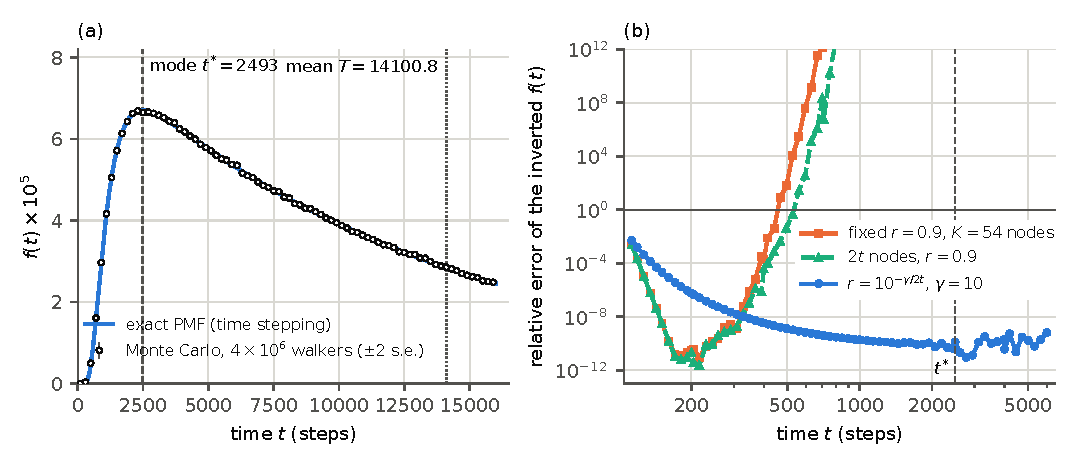
\includegraphics[width=\textwidth]{s3_methods_validation.pdf}
\caption{Corner-to-corner first passage on the square lattice, $N=35$, $q=0.8$, discrete time. (a)~Exact PMF from
time stepping (line) and histogram of $4\times10^{6}$ simulated walkers in bins of 200 steps (circles; bars are
$\pm2$ standard errors and are smaller than the symbols). Dashed line: mode $\tmode=2493$; dotted line: mean
$\MF=14\,100.8$. (b)~Relative error of three numerical inversions of the generating function against the exact PMF:
the trapezoidal rule on a circle of fixed radius $r=0.9$ truncated after $K=54$ nodes, the same rule with all $2t$
nodes, and the rule \eqref{s3_methods:eq-aw} with $\gamma=10$. The two fixed-radius curves leave the frame near
$t=700$; at $\tmode$ (dashed) the truncated fixed-radius rule returns $3.6\times10^{93}$.}
% src: code/article/s3_methods_validation.py; data/article/s3_methods_validation.json; data/article/s3_methods_mc_times.npz
\label{s3_methods:fig-aw}
\end{figure}

\subsection{Discrete and continuous time; parity}\label{sup_methods:ssec-parity}

In the 54 cases computed by both discrete and continuous routes at $q=0.8$ ($\dd=1,2,3$; \CC, \CtM, \MtC),
$\tmode=\tmodec/q+c$ with $-3.05\le c\le-0.22$ steps, and $-2.81\le c\le-0.52$ in the 17 cases of the second
implementation; the relative difference is below $10^{-4}$ for all $N\ge100$.
% src: data/msc_modes/fit_results.json (discrete_vs_continuous_offsets, max_abs_offset_steps); data/msc_modes_verify/analysis.json (summary_d2.offsets, summary_d3.offsets); data/article/s3_methods_validation.json (stored_runs_summary.discrete_vs_continuous_offset_q0.8)
The offset of the interpolated maximiser is $-0.45$ steps for the chain and drifts slowly with $N$ for $\dd\ge2$
(from $-0.56$ to $-1.01$ for $\dd=2$, $N=5$ to $200$, and from $-1.05$ to $-2.59$ for $\dd=3$, $N=5$ to $100$;
Fig.~\ref{s3_methods:fig-parity}(b)); whether it stays bounded as $N\to\infty$ is not established.
% src: data/msc_modes/fit_results.json (discrete_vs_continuous_offsets, offset_refined)
Other activities follow from the scaling with $q$ (Table~\ref{appC_tables:tab-activity}).

If $q\le\tfrac12$ no component of $\pmf$ alternates in sign, and at $q=0.8$ alternating components decay at least as
fast as $0.6^{t}$ (Proposition~\ref{s2_model:prop-structure}(d)). At $q=1$ parity is visible. On the chain only a
cancelled move at the reflecting end changes the parity of position plus time, the values of $\pmf$ at even and at
odd $t$ lie on two branches, the maximum of the even branch exceeding that of the odd branch by $4.0\%$ at $N=51$
(Fig.~\ref{s3_methods:fig-parity}(a)) and by $1.0\%$ at $N=201$, and the raw argmax is biased: $N=51$ gives $832$
against $\tmodec=849.9$, and $N=201$ gives $13\,332$ against $13\,398.0$. The two-step average
$\tfrac12[\pmf(t)+\pmf(t+1)]$ is maximal at $t=848$ and $t=13\,398$.
% src: data/article/derived_checks.json (B_parity_branches_chain_q1: larger_branch_maximum_over_smaller_minus_1); data/msc_modes/summary_tables.md (Table Q); data/article/s3_methods_validation.json (stored_runs_summary.parity_q1_1d, discrete_runs.q1_cases)
For $\dd=2$ and $q=1$ the PMF has a ripple at its peak, with two local maxima two steps apart ($t=678$ and $680$ at
$N=21$; also at $N=15$ and $N=51$, but not at $N=101$); for $\dd=3$ none was seen. Exact certificates confirm and
complete this: for $2\le N\le160$ the ripple occurs exactly at 16 sizes, among them 15, 21 and 51 but not 101, and
for $\dd=3$, $2\le N\le60$, never (Theorem~\ref{s6b_rigorous:thm-finite}, computer-assisted).
% src: data/msc_modes/discrete_modes.jsonl (local_maxima_first10); data/msc_modes_verify/analysis.json (discrete_unimodal.multi_max_q_1); data/msc_modes_verify/extra.json (q1_2d_N21_local_maxima_t)

\begin{figure}[tbp]
\centering
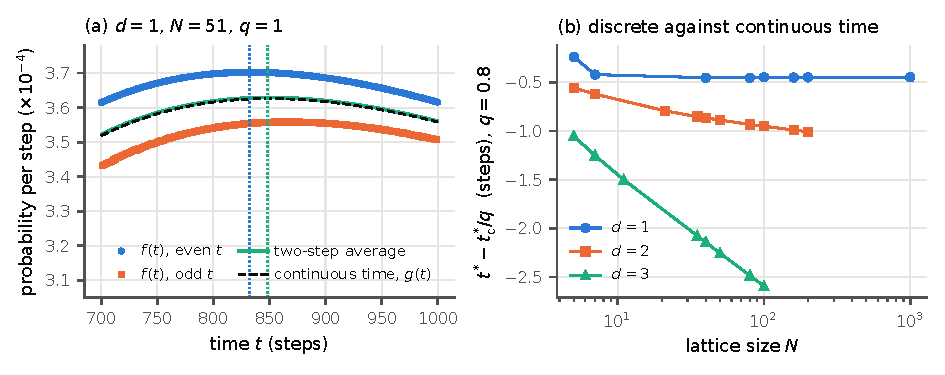
\includegraphics[width=\textwidth]{s3_methods_parity.pdf}
\caption{(a)~Parity at $q=1$: exact PMF of the one-dimensional chain (reflecting end to absorbing end, $N=51$) for
$700\le t\le1000$. Values at even $t$ (circles) and odd $t$ (squares) lie on two branches; the two-step average
(solid line) follows the continuous-time density at unit rate (dashed). Dotted vertical lines: raw argmax ($t=832$)
and maximiser of the two-step average. (b)~Difference, in steps, between the interpolated maximiser of the
discrete-time PMF at $q=0.8$ (three-point parabola through the exact values) and $\tmodec/q$, for corner-to-corner
transport in $\dd=1,2,3$ against $N$.}
% src: code/article/s3s6_modes_figures.py; data/msc_modes/pmf/pmf_d1_CC_N51_q1.0.npz; data/msc_modes/fit_results.json (discrete_vs_continuous_offsets)
\label{s3_methods:fig-parity}
\end{figure}

\subsection{The certificate of the global mode in practice}\label{sup_methods:ssec-certificate}

In the third time-stepping code the vectors $u_k=\Qm^{k}\ve_{\vo}$ and $v_k=\Qm^{k}r$ are advanced alternately;
$\pmf(2k+1)=u_k^{\T}v_k$ and $\pmf(2k+2)=u_{k+1}^{\T}v_k$ are sums of non-negative terms; and the run stops at the
first $k$ (tested every 16 steps) with $\|u_k\|\,\|v_k\|<(1-10^{-6})\max_{t\le2k}\pmf(t)$, so that $\tcert=2k+1$. The
cost is that of one time-stepping run of length $\tcert$. At the largest sizes $N=1000$, $401$ and $100$ for
$\dd=1,2,3$, $\tcert=584\,097$, $478\,369$ and $72\,673$ (up to $4.2\,\tmode$ for the smallest lattices).
% src: data/article/s3_methods_certificate.json (all_runs, CC_q0.8_d1, CC_q0.8_d2, CC_q0.8_d3, examples); data/article/s3_methods_certificate.jsonl (t_cert, t_cert_over_mode); code/article/s3_methods_certificate.py
\emph{Round-off.} The certificate has a relative margin of at least $10^{-6}$. The integer maximiser on
$\{1,\dots,\tcert-1\}$ is found by comparing computed values. For the 97 corner-to-corner runs at $q\in\{0.5,0.8,1\}$
the modes are also certified in exact arithmetic (Section~\ref{s3_methods:ssec-unimodal}). For the other 96 runs (the
placements \CtM, \MtC{} and \EXIT, and corner to corner at $q=0.3$ and $0.9$) we use an a-priori bound of the round-off
of route~A. Each component of $\rho_{t+1}$ is computed as a sum of at most $2\dd+1$ products of non-negative numbers,
each product rounded once and the sum rounded at most $2\dd$ times, with stored coefficients $q/(2\dd)$ and
$1-q+\frac{q}{2\dd}n$ ($n$ the number of cancelled directions) whose relative error $e$ against the exact values for the
exact activity is computed in rational arithmetic. Hence every computed component equals
$\sum_{\vy}\Qm(\vx,\vy)\tilde\rho_t(\vy)(1+\epsilon_{\vy})$ with $|\epsilon_{\vy}|\le\delta:=(1+u)^{2\dd+1}(1+e)-1$, $u=2^{-53}$,
and by induction, since $\Qm$ is non-negative, every computed $\pmf(t)$ lies between $(1-\delta)^{t}$ and
$(1+\delta)^{t}$ times the exact value (times $(1\mp u)^{m-1}$ for the sum over the $m$ target sites of \EXIT);
underflow adds an absolute error below $10^{-300}$. In these runs $\delta\le1.0\times10^{-15}$. The computed maximiser is
the exact one if every other computed value, multiplied by the upper factor at the maximiser, stays below the computed
maximum multiplied by the lower factor at its own time; this holds in all 96 runs. The smallest relative gap between
the maximum and any other computed value is $6.59\times10^{-11}$ ($\dd=2$, $N=141$, centre to corner), the relative
allowance $1-L(\tcert-1)/U(\tmode)$, where $U(t)$ and $L(t)$ denote the upper and lower factors, is at most $9.2\times10^{-11}$ (at $\dd=2$, $N=101$, $q=0.3$,
$\tmode=60\,187$), and in every run the gap exceeds the allowance, by a factor of at least $1.09$. The round-off of the
tail bound (norms of vectors of up to $10^{6}$ components) is below $2\times10^{-10}$, far below its margin. As a
consistency check, two evaluations of the same $\pmf(t)$ in the certificate code from different pairs of vectors,
$u_k^{\T}v_k$ and $u_{k+1}^{\T}v_{k-1}$, differ by at most $1.2\times10^{-15}$ in relative terms; this measures the
agreement of two evaluations, not the accumulated round-off, which is larger (see below).
% src: data/article/s3_methods_certificate_roundoff.json (n_runs_checked_here, n_certified_against_roundoff, max_delta_per_step, min_rel_gap_checked, max_roundoff_allowance_rel, min_gap_over_allowance, max_tail_roundoff_rel, rows); code/article/s3_methods_certificate_roundoff.py; data/article/s3_methods_certificate.jsonl (margin_rel, roundoff_rel_all_t)

One further size of the chain, $N=10\,240$, was certified with a compiled stepper: $\tcert=61\,300\,289$
($1.40\,\tmode$) and the maximiser is $\tmode=43\,679\,969$, the value located by route~B.
% src: data/article/s3_methods_certificate_chain_N10240.json (t_cert, t_cert_over_mode, mode, mode_equals_expected, certified); code/article/s3_methods_certificate_chain.c
At this size the maximum is too flat for the stepping to resolve the integer: neighbouring values of $\pmf$ differ
by $1.7\times10^{-16}$ in relative terms, whereas the stepped values, compared with the closed form
\eqref{s5_modes:eq-1d-pmf} in multi-precision arithmetic, carry an accumulated round-off of $1.1\times10^{-10}$ at
the mode (at most $1.5\times10^{-10}$ over the run).
% src: data/article/s3_methods_certificate_chain.json (multi_precision.gap_rel_to_larger_neighbour_50_digits; stepper_against_closed_form: rel_err_at_mode, whole_run.max_abs_rel_err); data/article/s3_methods_certificate_chain_N10240_probes.txt
The stepping is therefore used only where its margin exceeds its worst-case round-off. All its operations act on
non-negative numbers, so the relative error of every stepped quantity grows by at most five units of round-off per
step, which gives the a-priori bound $3.4\times10^{-8}$ for the whole run; underflow affects only components below
$10^{-300}$. Beyond $\tcert$ the bound (b) lies below the maximum by a relative $1.1\times10^{-6}$, and for
$t<\tcert$ outside a window of $\pm20\,000$ steps around the maximiser the stepped values lie below it by at least
$1.5\times10^{-7}$; both statements survive the a-priori bound. Inside the window the increments
$\pmf(t+1)-\pmf(t)$ of \eqref{s5_modes:eq-1d-pmf}, evaluated in 60-digit arithmetic at all $40\,001$ times (24
slowest terms; the omitted ones are bounded by $10^{-428}$, the smallest increment being $10^{-24}$), are positive up
to $\tmode-1$ and negative from $\tmode$ on. The same comparison shows that accumulated round-off is common to
neighbouring times: the relative error of the stepped values varies by $1.6\times10^{-15}$ within 60 steps of the mode
and by $3.8\times10^{-14}$ over the window. The a-priori comparison used for the 96 runs above
does not rely on this observation.
% src: data/article/s3_methods_certificate_chain.json (a_priori_roundoff.delta; part1_beyond_t_cert; part2_below_t_cert_outside_window; part3_window_closed_form: n_t, terms_kept, log10_tail_bound_on_increment, log10_smallest_abs_increment, increments_positive_for_t_below_mode, increments_negative_from_mode_on; certified_global_maximiser; stepper_against_closed_form: near_mode.max_abs_variation_of_rel_err, stored_window.max_abs_variation_of_rel_err); code/article/s3_methods_certificate_chain_check.py (derivation of the a-priori bound)

\subsection{Unimodality on the chain and the observed single maximum}

\begin{proposition}[Unimodality on the chain]\label{s3_methods:prop-1d-unimodal}
Let $\dd=1$, start at the reflecting end $0$ and target $N-1$, and let $\lambda_m=1-q+q\cos\omega_m$,
$\omega_m=(2m-1)\pi/(2N-1)$, be as in Proposition~\ref{s5_modes:prop-1d}. Then
\begin{equation}\label{s3_methods:eq-1d-product}
  \Ftil_q(z)=\prod_{m=1}^{N-1}\frac{(1-\lambda_m)\,z}{1-\lambda_m z},\qquad
  \Fhat(s)=\prod_{m=1}^{N-1}\frac{1-\cos\omega_m}{s+1-\cos\omega_m}.
\end{equation}
Consequently (i) the continuous-time first-passage time is a sum of $N-1$ independent exponential variables and
its density $\gd$ is log-concave, hence unimodal, for every $N$; (ii) if $q\,[1+\cos(2\pi/(2N-1))]\le1$, in
particular if $q\le\tfrac12$, the discrete first-passage time is a sum of $N-1$ independent geometric variables and
$\pmf$ is log-concave ($\pmf(t)^{2}\ge\pmf(t-1)\pmf(t+1)$), hence unimodal.
\end{proposition}

\begin{proof}
Here $\Qm$ is tridiagonal on $\{0,\dots,N-2\}$ with off-diagonal entries $q/2$, and only site $N-2$ is adjacent to
the target, so $\Ftil_q(z)=z\,\tfrac q2\,[(I-z\Qm)^{-1}]_{0,N-2}$. By Cramer's rule the corner entry of the inverse of a
tridiagonal matrix is the product of its off-diagonal entries, up to sign, divided by the determinant:
$[(I-z\Qm)^{-1}]_{0,N-2}=(zq/2)^{N-2}/\det(I-z\Qm)$. The eigenvalues of $\Qm$ are the $\lambda_m$
(Proposition~\ref{s5_modes:prop-1d}), so $\det(I-z\Qm)=\prod_m(1-\lambda_m z)$ and
$\Ftil_q(z)=(zq/2)^{N-1}/\prod_m(1-\lambda_m z)$. Since $\Ftil_q(1)=1$, $(q/2)^{N-1}=\prod_m(1-\lambda_m)$, which gives
the first product; the second follows from \eqref{s2_model:eq-transform}. (Numerically, both products agree with
direct solves to $6\times10^{-13}$.)
% src: data/article/s3_methods_validation.json (prop_1d_product)
A factor $\nu/(s+\nu)$ is the transform of an exponential density, and a factor $(1-\lambda)z/(1-\lambda z)$ with
$0\le\lambda<1$ is the generating function of a geometric variable on $\{1,2,\dots\}$; the smallest $\lambda_m$ is
$1-q-q\cos(2\pi/(2N-1))$. Exponential densities and geometric distributions are log-concave, and a density (lattice
distribution) is log-concave if and only if it is strongly unimodal, that is, if its convolution with every unimodal
density (lattice distribution) is unimodal \citep{Ibragimov1956,KeilsonGerber1971}. The class of strongly unimodal
laws is closed under convolution. Induction over the factors therefore shows that $\gd$ in case (i) and $\pmf$ in case
(ii) are log-concave and unimodal.
\end{proof}

The product form is the classical passage-time representation for birth-and-death processes
\citep{KarlinMcGregor1959,Keilson1971}, and in discrete time that of \citet{Fill2009}. It does not cover $q=0.8$ at
large $N$, where some $\lambda_m$ are negative, nor starts inside the chain, and at $q=1$ the conclusion is false
(Proposition~\ref{s6b_rigorous:prop-1dfail}). Section~\ref{s6b_rigorous:sec} of the main text extends it.

\begin{observation}[Single maximum for point targets]\label{s3_methods:obs-unimodal}
In every computation on the clean lattice with a point target and $q\le0.9$, the first-passage PMF or the
unit-rate density has exactly one local maximum on the range examined:
\begin{enumerate}
\item[(a)] 35 full-support runs of route A ($\Sv<10^{-12}$ at the end; $q=0.5$ and $0.8$; \CC, \CtM, \MtC; $N\le101$,
$35$ and $15$ for $\dd=1,2,3$; 27 of them with $\dd\ge2$) have one local maximum and no local minimum, as do 26 runs
of the second time-stepping code (20 with $\dd\ge2$);
% src: data/msc_modes/full_tail.json; data/msc_modes_verify/analysis.json (discrete_unimodal.full_support_runs); data/article/s3_methods_validation.json (stored_runs_summary.full_support_runs)
\item[(b)] all 151 point-target runs of route A with $q\le0.9$ (112 with $\dd\ge2$) have one local maximum on
$1\le t<\tcert$ and decrease monotonically from the mode to $\tcert$, beyond which $\pmf$ stays below its maximum
by Proposition~\ref{s3_methods:prop-certificate}; all 150 point-target runs with $q\le0.9$ of the second code have
one local maximum and decrease monotonically from the mode to the end of the run (as do its 15 runs of the exit
geometry);
% src: data/article/s3_methods_certificate.json (point_target_q_le_0.9: n_single_local_maximum_below_t_cert, n_monotone_from_mode_to_t_cert); data/msc_modes/discrete_modes.jsonl (n_local_maxima, monotone_after_mode); data/article/derived_checks.json (C_second_stepper_runs); data/msc_modes_verify/discrete.jsonl
\item[(c)] in all 156 two- and three-dimensional cases of route C, $\gd'$ changes sign exactly once, from positive to
negative, on a grid of four points per octave that starts below $0.22\,\tmodec$ and ends at $15\,q\MF$
(83 cases) or at 256 times a first estimate of the mode (73 cases), whichever is smaller. The grid always extends
beyond $53\,\tmodec$, but for the largest three-dimensional lattices that is only $0.03\,q\MF$ (\MtC, $N=1281$) to
$0.11\,q\MF$ (\CC, $N=4096$);
% src: data/msc_modes/laplace_modes.jsonl (n_sign_changes_down, n_sign_changes_up, grid_tmin, grid_tmax); code/msc_modes/03_run_laplace.py (find_mode_talbot); data/article/s3_methods_validation.json (stored_runs_summary.continuous_time_sign_scan)
\item[(d)] for corner-to-corner transport, the pole sum of route P has $\gd'>0$ on $[0.6\,\tmodec,\tmodec)$ and
$\gd'<0$ on $(\tmodec,15\,q\MF]$ at all 65 sizes ($N\le16\,777\,216$ for $\dd=2$, $N\le4096$ for $\dd=3$).
% src: data/msc_modes_verify/monotonicity_poles.json; code/msc_modes_verify/v10_tables.py; data/msc_modes_verify/poles.jsonl
\end{enumerate}
\end{observation}

Only (a) covers the whole support; the details are in Table~\ref{appC_tables:tab-unimodal}. Most of the observation is
a theorem: items (c) and (d) follow from Theorem~\ref{s6b_rigorous:thm-unimodal}(i), and items (a) and (b) from
Theorems~\ref{s6b_rigorous:thm-45}, \ref{s6b_rigorous:thm-finite} and~\ref{s6b_rigorous:thm-1d}(c) for every run except
the two corner-to-corner runs at $q=0.9$ with $\dd=2$, $N=101$ and $\dd=3$, $N=31$, which lie outside the proved
ranges. Extended targets are different: for \EXIT{} in one dimension at $N=11$ a parity ripple with four local maxima
at very short times ($t=5,7,9,11$) appears already at $q=0.8$; the certificate applies there as well and returns the
global one.
% src: data/msc_modes/discrete_modes.jsonl (geo = EXIT, d = 1, N = 11, q = 0.8: n_local_maxima = 4, local_maxima_first10); data/article/s3_methods_certificate.json (exit)

\subsection{Numerical inversion of a generating function}\label{s3_methods:ssec-aw}

Inverting the generating function $\Ftil$ numerically is a tempting alternative to time stepping, and it has a
pitfall of general interest. The rule of \citet{AbateWhitt1992ORL,AbateWhitt1992QS} is the trapezoidal rule on a
circle of radius $r<1$ with $2t$ nodes and a radius that depends on $t$:
\begin{equation}\label{s3_methods:eq-aw}
  \pmf(t)\;\approx\;\frac{1}{2t\,r^{t}}\sum_{k=1}^{2t}(-1)^{k}\,\operatorname{Re}\Ftil\bigl(r\,\eu^{\iu\pi k/t}\bigr),
  \qquad r=10^{-\gamma/(2t)} .
\end{equation}
Inserting $\Ftil(z)=\sum_{m}\pmf(m)z^{m}$ and using that $\sum_{k=1}^{2t}(-1)^{k}\eu^{\iu\pi km/t}$ equals $2t$ if
$m\equiv t \pmod{2t}$ and $0$ otherwise shows that the right-hand side equals
$\sum_{j\ge0}\pmf\bigl((2j+1)t\bigr)\,r^{2jt}$ exactly. The error of \eqref{s3_methods:eq-aw} is therefore the aliasing
sum $\sum_{j\ge1}\pmf((2j+1)t)\,10^{-\gamma j}\le10^{-\gamma}/(1-10^{-\gamma})$, and the prefactor $r^{-t}=10^{\gamma/2}$ that
multiplies round-off does not grow with $t$.

Two simplifications that look harmless are fatal at large $t$: a radius fixed independently of $t$, and a sum
truncated after a fixed number $K<t-1$ of nodes. With a fixed radius the bracket has to cancel down to
$t\,r^{t}\pmf(t)$, with $0.9^{1000}=1.7\times10^{-46}$, from terms of order $\Ftil(0.9)=1.4\times10^{-16}$.
% src: data/article/s3_methods_validation.json (inversion.summary: r_pow_t_at_1000; generating_function: Ftil_at_0.9)
Figure~\ref{s3_methods:fig-aw}(b) shows the outcome for $N=35$, $q=0.8$, for the rule with $r=0.9$ and the sum
truncated after $K=54$ nodes (with the term $\frac12\Ftil(r)$ added). These two values are one example of a fixed radius
and a fixed truncation, not a tuned choice; the rule with the same radius and all $2t$ nodes, shown as well, separates
the effect of the radius from that of the truncation. Its relative error is below $4\times10^{-4}$ for
$150\le t\le400$ ($2\times10^{-4}$ at $t=400$). It passes $1\%$ at $t=417$ and exceeds $100\%$ at every $t$ from $455$
on that we examined (all integers up to $700$ and 40 larger values); it returns $4.3\times10^{23}$ at $t=1000$, where
$\pmf=3.59\times10^{-5}$, and $3.6\times10^{93}$ at the modal time $t=2493$, where $\pmf=6.70\times10^{-5}$. With all
$2t$ nodes but the fixed radius the breakdown comes slightly later (error above $100\%$ from $t=535$ on,
$3.2\times10^{85}$ at the modal time). The rule \eqref{s3_methods:eq-aw} with $\gamma=10$ has relative error
$1.3\times10^{-10}$ at the modal time and at most $6.4\times10^{-10}$ for $1000\le t\le6000$; on the rising flank,
where $\pmf(3t)\gg\pmf(t)$, it is larger ($1.5\times10^{-8}$ at $t=309$), exactly as the aliasing sum predicts.
% src: data/article/s3_methods_validation.json (inversion.summary, inversion.rows); data/msc_modes/validation.json (abate_whitt_check); data/msc_modes_verify/misc.json (abate_whitt)
At other sizes, all at $q=0.8$, the truncated fixed-radius rule is off by $1.6\%$ at the modal time for $\dd=2$,
$N=9$ ($\tmode=136$), by $19\%$ for the chain with $N=21$ ($\tmode=174$), and returns $6.4\times10^{19}$ for $\dd=2$,
$N=20$ ($\tmode=765$, $\pmf=2.42\times10^{-4}$).
% src: data/article/s3_methods_inversion_other_sizes.json (fixed_radius_rule_r0.9_K54_at_modal_time); code/article/s3_methods_inversion_other_sizes.py
For the sizes of this article, inversion of $\Ftil$ is unnecessary: time stepping is simpler and exact, and for larger
lattices the Laplace transform is inverted instead (route C).

% appA_proofs.tex -- Supplementary Section S3: proofs of the mean first-passage time formulas (zero-based sites).
% Every displayed identity of this section is evaluated, in the form printed here, by
%   code/article/appA_proofs_check.py  ->  data/article/appA_proofs_check.json   (51 checks, 0 failed)
\section{Proofs of the mean first-passage time formulas}\label{appA_proofs:sec}

This section proves Theorems~\ref{s4_mfpt:thm-cosine}, \ref{s4_mfpt:thm-single} and~\ref{s4_mfpt:thm-pair},
Corollary~\ref{s4_mfpt:cor-resistance} and Proposition~\ref{s4_mfpt:prop-3d}. The inputs are
Proposition~\ref{s2_model:prop-pinv} and three elementary lemmas. The symbols $G_k$, $g_k$, $H_k$, $G_{kj}$,
$g_{kj}$, $\Gamma$, $O_N$ and $u_k$ are local to this section ($G_k$ is an inner sum, not the Green's function
$\Glap$). Throughout, $N\ge2$, $q\in(0,1]$, sites are
zero-based, and for $k=0,\dots,N-1$ and $m\in\mathbb Z$
\[
  \angk{k}=\frac{\pi k}{N},\qquad \ck{k}=\cos\frac{\pi k}{2N},\qquad \sk{k}=\sin\frac{\pi k}{2N},\qquad
  \thk{k}{m}=\frac{\pi k(2m+1)}{2N},
\]
so that $1-\cos\angk{k}=2\sk{k}^{2}$ and $1+\cos\angk{k}=2\ck{k}^{2}$. For $k\ge1$, $\sigk{k}=2-\cos\angk{k}>1$ and
$\phk{k}=\arcosh\sigk{k}>0$; since $\cosh\varphi=1+2\sinh^{2}(\varphi/2)$,
\begin{equation}\label{appA_proofs:eq-half-angle}
  \sinh\frac{\phk{k}}{2}=\sk{k},\qquad \coth\frac{\phk{k}}{2}=\frac{\sqrt{1+\sk{k}^{2}}}{\sk{k}} .
\end{equation}

All identities displayed below were evaluated numerically in the form printed here. The formulas, computed to
$40$ digits, were compared with exact rational solutions of $(I-\Qm)h=\one$ for the walk built from its rules
($\dd=1$: $N\le12$; $\dd=2$: $N\le9$, including all $1848$ ordered pairs with $N\le5$ at two values of $q$;
$\dd=3$: $N\le4$) and with double-precision sparse solves ($\dd=2$: $N=16,35,36,100,101$; $\dd=3$: $N=5,\dots,12$):
$51$ checks, none failed. The largest deviation is $8.5\times10^{-36}$ in the multiprecision comparisons and
$1.4\times10^{-12}$ against the sparse solves; the double-precision matrix identities (eigenvectors,
pseudo-inverses, resistances) hold to $3\times10^{-14}$.
% src: data/article/appA_proofs_check.json (n_checks, n_failed, summary, checks[].max_deviation) ; code/article/appA_proofs_check.py

\subsection{Spectrum of the walk and the cosine sum}

\begin{lemma}[Spectrum of the reflecting walk]\label{appA_proofs:lem-spectrum}
Let $\mathsf T$ be the $N\times N$ matrix with $\mathsf T(m,m\pm1)=\tfrac12$ for $0\le m,m\pm1\le N-1$,
$\mathsf T(0,0)=\mathsf T(N-1,N-1)=\tfrac12$ and zero otherwise.  Then
$\psi_k(m)=\sqrt{\alk{k}/N}\,\cos\thk{k}{m}$, $k=0,\dots,N-1$, is an orthonormal eigenbasis,
$\mathsf T\psi_k=\cos(\pi k/N)\,\psi_k$, and
$\Pm=(1-q)I+\frac{q}{\dd}\sum_{i=1}^{\dd}\mathsf T^{(i)}$, where $\mathsf T^{(i)}$ acts as $\mathsf T$ on the $i$-th coordinate.
Hence the products $\prod_i\psi_{k_i}(x_i)$ diagonalise $\Pm$ with
$1-\lambda_{\vk}=\frac{2q}{\dd}\sum_i\sk{k_i}^{2}$.
\end{lemma}

\begin{proof}
Put $u_k(m)=\cos\thk{k}{m}$ for $m\in\mathbb Z$. The addition formula gives
$u_k(m-1)+u_k(m+1)=2\cos(\angk{k})\,u_k(m)$ for every $m$. Because $\thk{k}{-1}=-\thk{k}{0}$ and
$\thk{k}{N}=2\pi k-\thk{k}{N-1}$,
\begin{equation}\label{appA_proofs:eq-bdry}
  u_k(-1)=u_k(0),\qquad u_k(N)=u_k(N-1).
\end{equation}
Hence $(\mathsf T u_k)(0)=\tfrac12[u_k(0)+u_k(1)]=\tfrac12[u_k(-1)+u_k(1)]=\cos(\angk{k})\,u_k(0)$, likewise at
$m=N-1$, and at the interior sites the eigenvalue equation is the addition formula itself. The $N$ eigenvalues
$\cos\angk{k}$ are distinct and $\mathsf T$ is symmetric, so the $u_k$ are mutually orthogonal. For $1\le k\le N-1$,
$\sum_{m=0}^{N-1}\cos^{2}\thk{k}{m}=\frac N2+\frac12\,\mathrm{Re}\sum_{m=0}^{N-1}\eu^{\iu\angk{k}(2m+1)}=\frac N2$,
because the geometric sum vanishes ($\eu^{2\iu N\angk{k}}=1$, $\eu^{2\iu\angk{k}}\ne1$); for $k=0$ the sum is $N$.
This gives the normalisation $\sqrt{\alk{k}/N}$. Finally, by the rule \eqref{s2_model:eq-P} an attempt along
coordinate $i$ has probability $q/\dd$; it changes $x_i$ by $\pm1$ with probability $\tfrac12$ each, unless the
walker would leave $\{0,\dots,N-1\}$, in which case nothing moves. That is $\mathsf T$ acting on the $i$-th
coordinate, so $\Pm=(1-q)I+\frac q\dd\sum_i\mathsf T^{(i)}$. The products are therefore eigenvectors with
$\lambda_{\vk}=1-q+\frac q\dd\sum_i\cos\angk{k_i}$, and $1-\cos\angk{k}=2\sk{k}^{2}$.
\end{proof}

As in \eqref{s2_model:eq-prop}, write $\phi_{\vk}(\vx)=\prod_i\psi_{k_i}(x_i)$. Since $\sum_i\sk{k_i}^{2}>0$ unless $\vk=\mathbf 0$, the eigenvalue
$0$ of $\Lm=I-\Pm$ is simple, and the pseudo-inverse inverts the other eigenvalues:
\begin{equation}\label{appA_proofs:eq-Lplus}
  \Lp_{\vx\vy}=\frac{\dd}{2q}\sum_{\vk\ne\mathbf 0}\frac{\phi_{\vk}(\vx)\,\phi_{\vk}(\vy)}{\sum_{i}\sk{k_i}^{2}},\qquad
  \phi_{\vk}(\vx)\,\phi_{\vk}(\vy)=\frac{1}{N^{\dd}}\prod_{i=1}^{\dd}\alk{k_i}\cos\thk{k_i}{x_i}\cos\thk{k_i}{y_i}.
\end{equation}

\begin{proof}[Proof of Theorem~\ref{s4_mfpt:thm-cosine}]
$\Pm$ is symmetric, stochastic and irreducible, so Proposition~\ref{s2_model:prop-pinv} applies with $\nn=N^{\dd}$.
Inserting \eqref{appA_proofs:eq-Lplus} into \eqref{s2_model:eq-pinv} gives \eqref{s4_mfpt:eq-cosine}; the factor
$1/q$ is explicit, so $q\,\MF_{\vo\to\va}$ does not depend on $q$. For opposite corners use
\begin{equation}\label{appA_proofs:eq-corner-cos}
  \cos\thk{k}{0}=\ck{k},\qquad \cos\thk{k}{N-1}=\cos\Bigl(\pi k-\frac{\pi k}{2N}\Bigr)=(-1)^{k}\ck{k}.
\end{equation}
The numerator of \eqref{s4_mfpt:eq-cosine} becomes $\prod_i\ck{k_i}^{2}\,[1-(-1)^{k_1+\dots+k_{\dd}}]$, which
vanishes when $k_1+\dots+k_{\dd}$ is even and equals $2\prod_i\ck{k_i}^{2}$ when it is odd. This is
\eqref{s4_mfpt:eq-cosine-cc}. For $\dd=1$, \eqref{s4_mfpt:eq-cosine} is the left-hand side of
\eqref{appA_proofs:eq-1d-sum} (because $\alk{k}=2$ and $2\sk{k}^{2}=1-\cos\angk{k}$), which equals $\hone(m,m')$ by
Lemma~\ref{appA_proofs:lem-1d} below; that lemma uses only Proposition~\ref{s2_model:prop-pinv} and
Lemma~\ref{appA_proofs:lem-spectrum}. In particular $q\,\TNd{1}=\hone(0,N-1)=N(N-1)$.
\end{proof}

\subsection{Two summation lemmas}

\begin{lemma}[Green's function of a ring]\label{appA_proofs:lem-ring}
Let $M\ge1$ be an integer and $\sigma=\cosh\varphi>1$ with $\varphi>0$.  For every integer $0\le m\le M$,
\begin{equation}\label{appA_proofs:eq-ring}
  \sum_{l=0}^{M-1}\frac{\cos(2\pi lm/M)}{\sigma-\cos(2\pi l/M)}=\frac{M\,\cosh\bigl((\tfrac M2-m)\varphi\bigr)}{\sinh\varphi\,\sinh(M\varphi/2)} ,
\end{equation}
and consequently, for every integer $0\le m\le 2N$,
\begin{equation}\label{appA_proofs:eq-ring-half}
  \sum_{j=0}^{N-1}\frac{\alk{j}\cos(\pi m j/N)}{\sigma-\cos(\pi j/N)}=\frac{2N\cosh\bigl((N-m)\varphi\bigr)}{\sinh\varphi\,\sinh N\varphi}-\frac{(-1)^{m}}{\sigma+1}.
\end{equation}
\end{lemma}

\begin{proof}
Let $A$ be the averaging operator on functions on the ring $\mathbb Z_M$, $(Af)(m)=\tfrac12[f(m-1)+f(m+1)]$. Its
eigenfunctions are $m\mapsto\eu^{2\pi\iu lm/M}$ with eigenvalues $\cos(2\pi l/M)\in[-1,1]$, so $\sigma-A$ is
invertible and
\[
  \bigl((\sigma-A)^{-1}\delta_0\bigr)(m)=\frac1M\sum_{l=0}^{M-1}\frac{\eu^{2\pi\iu lm/M}}{\sigma-\cos(2\pi l/M)},
\]
where $\delta_0$ is the indicator of the site $0$. Define
$\Gamma(m)=\cosh\bigl((\tfrac M2-m)\varphi\bigr)/\bigl(\sinh\varphi\,\sinh(M\varphi/2)\bigr)$ for $0\le m\le M$. Then
$\Gamma(0)=\Gamma(M)$, so $\Gamma$ is a function on $\mathbb Z_M$. For $1\le m\le M-1$,
$\cosh((\tfrac M2-m+1)\varphi)+\cosh((\tfrac M2-m-1)\varphi)=2\cosh\varphi\,\cosh((\tfrac M2-m)\varphi)$, that is,
$((\sigma-A)\Gamma)(m)=0$. At $m=0$ the two neighbours are $1$ and $M-1$, $\Gamma(M-1)=\Gamma(1)$, and
\[
  \sigma\,\Gamma(0)-\Gamma(1)=\frac{\cosh\varphi\,\cosh\frac{M\varphi}{2}-\cosh\bigl(\frac{M\varphi}{2}-\varphi\bigr)}
  {\sinh\varphi\,\sinh\frac{M\varphi}{2}}=1 .
\]
Hence $(\sigma-A)\Gamma=\delta_0$, so $\Gamma=(\sigma-A)^{-1}\delta_0$, and taking real parts gives
\eqref{appA_proofs:eq-ring}. For \eqref{appA_proofs:eq-ring-half} take $M=2N$: the summand
$F(l)=\cos(\pi ml/N)/(\sigma-\cos(\pi l/N))$ satisfies $F(2N-l)=F(l)$, so
$\sum_{l=0}^{2N-1}F(l)=F(0)+F(N)+2\sum_{l=1}^{N-1}F(l)=\sum_{j=0}^{N-1}\alk{j}F(j)+(-1)^{m}/(\sigma+1)$.
\end{proof}

\begin{remark}
Subtracting the term $j=0$ from \eqref{appA_proofs:eq-ring-half} and dividing by two gives
\[
  \sum_{j=1}^{N-1}\frac{\cos(\pi mj/N)}{\sigma-\cos(\pi j/N)}=\frac{N\cosh\bigl((N-m)\varphi\bigr)}{\sinh\varphi\,\sinh N\varphi}
  -\frac12\Bigl[\frac{1}{\sigma-1}+\frac{(-1)^{m}}{\sigma+1}\Bigr],
\]
which is Eq.~(E1) of \citet{Giuggioli2020}, written there with Chebyshev polynomials
($\cosh n\varphi$ and $\sinh n\varphi/\sinh\varphi$ are the Chebyshev polynomials of the first and second kind
in $\sigma$). \citet{EssamWu2009} use an equivalent summation lemma, proved by
contour integration. So Lemma~\ref{appA_proofs:lem-ring} is known; the short proof is included to keep the
section self-contained. The range $0\le m\le2N$ is sharp: the left-hand side of \eqref{appA_proofs:eq-ring-half}
is even and $2N$-periodic in $m$, the right-hand side is not, and at $m=-1$ or $m=2N+1$ the two sides differ by
exactly $4N$, because $\cosh(N+1)\varphi-\cosh(N-1)\varphi=2\sinh N\varphi\,\sinh\varphi$. For other $m$, first
reduce $m$ to $[0,2N]$.
% src: data/article/appA_proofs_check.json (labels appA_proofs:eq-E1, "appA_proofs:eq-ring-half (range)": violations 4N at sigma = 3)
\end{remark}

\begin{lemma}[One-dimensional hitting times]\label{appA_proofs:lem-1d}
For the chain $\mathsf T$ of Lemma~\ref{appA_proofs:lem-spectrum} the mean hitting time from $m$ to $m'$ is
$\hone(m,m')$ of \eqref{s4_mfpt:eq-1d}, and
\begin{equation}\label{appA_proofs:eq-1d-sum}
  \sum_{j=1}^{N-1}\alk{j}\,\frac{\cos^{2}\thk{j}{m'}-\cos\thk{j}{m}\cos\thk{j}{m'}}{1-\cos(\pi j/N)}=\hone(m,m').
\end{equation}
In particular (take $m=0$, $m'=N-1$)
\begin{equation}\label{appA_proofs:eq-cot}
  \sum_{\substack{1\le j\le N-1\\ j\ \mathrm{odd}}}\cot^{2}\frac{\pi j}{2N}=\frac{N(N-1)}{2}.
\end{equation}
\end{lemma}

\begin{proof}
Fix $m'$ and put $h(m)=\hone(m,m')$. For $m\le m'$ this is $h(m)=m'(m'+1)-m(m+1)$. It satisfies $h(m')=0$; for
$1\le m\le m'-1$, $\tfrac12[h(m-1)+h(m+1)]=h(m)-1$, because $(m-1)m+(m+1)(m+2)=2m(m+1)+2$; and at $m=0$ (if
$m'\ge1$), $(\mathsf Th)(0)=\tfrac12[h(0)+h(1)]=h(0)-1$, because $h(1)=h(0)-2$. These equations involve only sites
$\le m'$. For $m\ge m'$ the function is the same expression after the reflection $m\mapsto N-1-m$,
$m'\mapsto N-1-m'$, which maps the chain to itself, so the equations at the sites $m>m'$ hold as well. Thus
$h(m')=0$ and $((I-\mathsf T)h)(m)=1$ for all $m\ne m'$, and by the uniqueness statement of
Proposition~\ref{s2_model:prop-pinv} (the chain $\mathsf T$ is symmetric, stochastic and irreducible) $h$ is the
mean hitting time. Identity \eqref{appA_proofs:eq-1d-sum} is \eqref{s2_model:eq-pinv} for $\mathsf T$, with
$\nn=N$ and $(I-\mathsf T)^{+}_{mm'}=\sum_{j\ge1}\psi_j(m)\psi_j(m')/(1-\cos\angk{j})$ from
Lemma~\ref{appA_proofs:lem-spectrum}. For \eqref{appA_proofs:eq-cot} take $m=0$, $m'=N-1$ and use
\eqref{appA_proofs:eq-corner-cos}: the summand vanishes for even $j$ and equals $2\ck{j}^{2}/\sk{j}^{2}$ for odd
$j$, and $\hone(0,N-1)=N(N-1)$.
\end{proof}

\subsection{Proof of Theorem~\ref{s4_mfpt:thm-single}}

\emph{Step 1 (splitting off the row $k=0$).} For $\dd=2$, $\sk{k}^{2}+\sk{j}^{2}=\tfrac12(2-\cos\angk{k}-\cos\angk{j})$,
and \eqref{s4_mfpt:eq-cosine-cc} reads
$\tfrac12\,q\,\TN=\sum_{(k,j)\ne(0,0)}\alk{k}\alk{j}\ck{k}^{2}\ck{j}^{2}[1-(-1)^{k+j}]/(2-\cos\angk{k}-\cos\angk{j})$.
In the row $k=0$ the denominator is $1-\cos\angk{j}$ and $\alk{0}\ck{0}^{2}=1$; in a row $k\ge1$ it is
$\sigk{k}-\cos\angk{j}$, $\alk{k}=2$, and $j$ runs over $0,\dots,N-1$. Therefore
\begin{equation}\label{appA_proofs:eq-split}
  \frac{q\,\TN}{2}=\sum_{j=1}^{N-1}\frac{\alk{j}\ck{j}^{2}\,[1-(-1)^{j}]}{1-\cos\angk{j}}+\sum_{k=1}^{N-1}2\ck{k}^{2}\,G_k,
  \qquad
  G_k:=\sum_{j=0}^{N-1}\frac{\alk{j}\ck{j}^{2}\,[1-(-1)^{k+j}]}{\sigk{k}-\cos\angk{j}} .
\end{equation}
By \eqref{appA_proofs:eq-1d-sum} with $m=0$, $m'=N-1$ the first sum equals $\hone(0,N-1)=N(N-1)$.

\emph{Step 2 (the inner sum).} Write $\ck{j}^{2}=\tfrac12[(1+\sigk{k})-(\sigk{k}-\cos\angk{j})]$ and
$(-1)^{j}=\cos(N\angk{j})$. Then
\[
  G_k=\frac{1+\sigk{k}}{2}\sum_{j=0}^{N-1}\frac{\alk{j}\,[1-(-1)^{k}\cos(N\angk{j})]}{\sigk{k}-\cos\angk{j}}
  -\frac12\sum_{j=0}^{N-1}\alk{j}\,[1-(-1)^{k+j}] .
\]
By \eqref{appA_proofs:eq-ring-half} with $m=0$ and with $m=N$,
\begin{align*}
  \sum_{j=0}^{N-1}\frac{\alk{j}}{\sigk{k}-\cos\angk{j}}&=\frac{2N\cosh N\phk{k}}{\sinh\phk{k}\,\sinh N\phk{k}}-\frac{1}{\sigk{k}+1},\\
  \sum_{j=0}^{N-1}\frac{\alk{j}\cos(N\angk{j})}{\sigk{k}-\cos\angk{j}}&=\frac{2N}{\sinh\phk{k}\,\sinh N\phk{k}}-\frac{(-1)^{N}}{\sigk{k}+1},
\end{align*}
and $\sum_{j=0}^{N-1}\alk{j}=2N-1$, $\sum_{j=0}^{N-1}\alk{j}(-1)^{j}=-(-1)^{N}$ (from
$\sum_{j=0}^{2N-1}(-1)^{j}=0$ and the symmetry $j\mapsto2N-j$). The terms containing $(-1)^{k+N}$ cancel, the
constants combine to $-N$, and
\begin{equation}\label{appA_proofs:eq-Gk}
  G_k=\frac{N\,(1+\sigk{k})\,[\cosh N\phk{k}-(-1)^{k}]}{\sinh\phk{k}\,\sinh N\phk{k}}-N .
\end{equation}

\emph{Step 3 (form (a)).} Since $\cosh(N-1)\varphi=\cosh N\varphi\cosh\varphi-\sinh N\varphi\sinh\varphi$ and
$\cosh\phk{k}=\sigk{k}$,
\begin{equation}\label{appA_proofs:eq-Bk}
  \Bk{k}=(1+\sigk{k})\,[\cosh N\phk{k}-(-1)^{k}]-\sinh\phk{k}\,\sinh N\phk{k},
  \qquad G_k=\frac{N\,\Bk{k}}{\sinh\phk{k}\,\sinh N\phk{k}} ,
\end{equation}
the second relation being \eqref{appA_proofs:eq-Gk} rewritten. Inserting it and $N(N-1)$ into \eqref{appA_proofs:eq-split} gives \eqref{s4_mfpt:eq-single-a}. The rows
$k\ge1$ were summed over all $j$, including $j=0$; no cancellation between different sectors of the double sum is
needed.

\emph{Step 4 (form (b)).} Because $(1+\cosh\varphi)/\sinh\varphi=\coth(\varphi/2)$,
$(\cosh N\varphi-1)/\sinh N\varphi=\tanh(N\varphi/2)$ and $(\cosh N\varphi+1)/\sinh N\varphi=\coth(N\varphi/2)$,
\eqref{appA_proofs:eq-Gk} reads
\begin{equation}\label{appA_proofs:eq-Gk-coth}
  G_k=N\Bigl[\coth\frac{\phk{k}}{2}\,g_k-1\Bigr],\qquad
  g_k=\coth\frac{N\phk{k}}{2}\ (k\ \text{odd}),\qquad g_k=\tanh\frac{N\phk{k}}{2}\ (k\ \text{even}).
\end{equation}
Moreover
\begin{equation}\label{appA_proofs:eq-csum}
  \sum_{k=1}^{N-1}\ck{k}^{2}=\frac{N-1}{2}+\frac12\sum_{k=1}^{N-1}\cos\angk{k}=\frac{N-1}{2},
\end{equation}
since the terms $k$ and $N-k$ of the cosine sum cancel. Hence, by \eqref{appA_proofs:eq-split},
\[
  q\,\TN=2N(N-1)+4N\sum_{k=1}^{N-1}\ck{k}^{2}\coth\frac{\phk{k}}{2}\,g_k-4N\cdot\frac{N-1}{2}
        =4N\sum_{k=1}^{N-1}\ck{k}^{2}\coth\frac{\phk{k}}{2}\,g_k ,
\]
which is \eqref{s4_mfpt:eq-single-S} by \eqref{appA_proofs:eq-half-angle}; note $N\phk{k}/2=N\arsinh\sk{k}$.

\emph{Step 5 (form (c)).} The summand of \eqref{s4_mfpt:eq-cosine-cc} is symmetric in $(k,j)$, and each pair with
$k+j$ odd has exactly one odd index. With $1/(\sk{k}^{2}+\sk{j}^{2})=2/(\sigk{k}-\cos\angk{j})$,
\begin{equation}\label{appA_proofs:eq-odd-even}
  q\,\TN=16\sum_{\substack{1\le k\le N-1\\ k\ \mathrm{odd}}}\ck{k}^{2}\,H_k,\qquad
  H_k:=\sum_{\substack{0\le j\le N-1\\ j\ \mathrm{even}}}\frac{\alk{j}\ck{j}^{2}}{\sigk{k}-\cos\angk{j}} .
\end{equation}
For $j=2l$ we have $\angk{j}=2\pi l/N$ and $\ck{j}^{2}=\cos^{2}(\pi l/N)$. The function
$l\mapsto\cos^{2}(\pi l/N)/(\sigk{k}-\cos(2\pi l/N))$ on $\mathbb Z_N$ is invariant under $l\mapsto N-l$ and
vanishes at $l=N/2$ when $N$ is even; hence $H_k$ equals its sum over all $l\in\mathbb Z_N$, for both parities of
$N$. Writing $\cos^{2}(\pi l/N)=\tfrac12[(1+\sigk{k})-(\sigk{k}-\cos(2\pi l/N))]$ and using
\eqref{appA_proofs:eq-ring} with $M=N$, $m=0$,
\begin{equation}\label{appA_proofs:eq-Hk}
  H_k=\frac{1+\sigk{k}}{2}\cdot\frac{N\cosh(N\phk{k}/2)}{\sinh\phk{k}\,\sinh(N\phk{k}/2)}-\frac N2
     =\frac N2\Bigl[\coth\frac{\phk{k}}{2}\coth\frac{N\phk{k}}{2}-1\Bigr].
\end{equation}
Next,
\begin{equation}\label{appA_proofs:eq-csum-odd}
  \sum_{\substack{1\le k\le N-1\\ k\ \mathrm{odd}}}\ck{k}^{2}=\frac N4\qquad\text{for every }N\ge2 .
\end{equation}
Indeed the left-hand side is half the number of odd $k<N$ plus $\tfrac12\,O_N$, where $O_N$ denotes the sum of
$\cos\angk{k}$ over the odd $k<N$. For even $N$ the number is $N/2$ and $O_N=0$, since $k\mapsto N-k$ maps odd
indices to odd indices and changes the sign of the cosine. For odd $N$ the number is $(N-1)/2$ and
$O_N=\tfrac12$. To see this, note that for odd $N$ the alternating sum
\[
  \sum_{k=0}^{N-1}(-1)^{k}\eu^{\iu\angk{k}}=\frac{1-(-1)^{N}\eu^{\iu\pi}}{1+\eu^{\iu\pi/N}}
\]
vanishes, so the sum of $\cos\angk{k}$ over the even $k$ (which includes the term $k=0$, equal to $1$) equals
$O_N$; on the other hand $k\mapsto N-k$ maps the even indices $k\ge2$ onto the odd ones and changes the sign of
the cosine, so the same sum equals $1-O_N$. In both cases the left-hand side is $N/4$. From
\eqref{appA_proofs:eq-odd-even}--\eqref{appA_proofs:eq-csum-odd},
\[
  q\,\TN=8N\sum_{k\ \mathrm{odd}}\ck{k}^{2}\Bigl[\coth\frac{\phk{k}}{2}\coth\frac{N\phk{k}}{2}-1\Bigr]=8N\,S_{\mathrm{odd}}-2N^{2}.
\]
Form (b) is $q\,\TN=4N\,(S_{\mathrm{odd}}+S_{\mathrm{even}})$. Comparing the two gives
$S_{\mathrm{odd}}-S_{\mathrm{even}}=N/2$ and then $q\,\TN=2N^{2}+8N\,S_{\mathrm{even}}$, which completes
\eqref{s4_mfpt:eq-half}. \qed

\begin{remark}
Form (a) contains $\cosh N\phk{k}$ and $\sinh N\phk{k}$, which are of size $\eu^{N\phk{k}}/2$. Since
$\phk{N-1}\to\arcosh3=1.7627$, the exponent $N\phk{N-1}$ passes the logarithm of the largest double-precision
number, $709.78$, between $N=402$ ($708.62$) and $N=403$ ($710.38$). Accordingly a direct double-precision
evaluation of \eqref{s4_mfpt:eq-single-a} is finite for every $N\le402$ (at $N=402$ it agrees with form (b) to
$5.7\times10^{-13}$) and returns no finite value at any size tested from $N=403$ on.
% src: data/article/appA_proofs_check.json (float64_overflow)
Forms (b) and (c) contain only $\tanh$ and $\coth$ and have no such limit.
\end{remark}

\subsection{Arbitrary start and target, resistance, and three dimensions}

\begin{proof}[Proof of Theorem~\ref{s4_mfpt:thm-pair}]
For $\dd=2$, \eqref{s4_mfpt:eq-cosine} reads
$q\,\MF_{\vo\to\va}=\sum_{(k,j)\ne(0,0)}2\alk{k}\alk{j}\,[\mathcal C_k(a_1,a_1)\mathcal C_j(a_2,a_2)-\mathcal C_k(o_1,a_1)\mathcal C_j(o_2,a_2)]/(2-\cos\angk{k}-\cos\angk{j})$.
In the row $k=0$, $\alk{0}=1$, $\mathcal C_0\equiv1$ and the denominator is $1-\cos\angk{j}$, so by
\eqref{appA_proofs:eq-1d-sum} this row contributes $2\,\hone(o_2,a_2)$. In the rows $k\ge1$ the sums over $j$ have
the form $\sum_{j=0}^{N-1}\alk{j}\cos\thk{j}{m}\cos\thk{j}{m'}/(\sigk{k}-\cos\angk{j})$. Now
\begin{equation}\label{appA_proofs:eq-prod}
  \cos\thk{j}{m}\cos\thk{j}{m'}=\tfrac12\bigl[\cos\bigl(|m-m'|\,\angk{j}\bigr)+\cos\bigl((m+m'+1)\,\angk{j}\bigr)\bigr],
\end{equation}
where $m_1=|m-m'|\in[0,N-1]$ and $m_2=m+m'+1\in[1,2N-1]$ have opposite parity. Both lie in the range of
\eqref{appA_proofs:eq-ring-half}; applying it to the two terms, the contributions $-(-1)^{m_1}/(\sigk{k}+1)$ and
$-(-1)^{m_2}/(\sigk{k}+1)$ cancel and
\begin{equation}\label{appA_proofs:eq-inner-pair}
  \sum_{j=0}^{N-1}\frac{\alk{j}\cos\thk{j}{m}\cos\thk{j}{m'}}{\sigk{k}-\cos\angk{j}}=N\,\Psi_k(m,m'),
\end{equation}
with $\Psi_k$ as in \eqref{s4_mfpt:eq-Psi}. Since $\alk{k}=2$ for $k\ge1$, this gives \eqref{s4_mfpt:eq-pair}.
\end{proof}

For $\vo=(0,0)$ and $\va=(N-1,N-1)$, \eqref{appA_proofs:eq-corner-cos} gives $\mathcal C_k(a_1,a_1)=\ck{k}^{2}$ and
$\mathcal C_k(o_1,a_1)=(-1)^{k}\ck{k}^{2}$, the numerators of $\Psi_k(N-1,N-1)$ and $\Psi_k(0,N-1)$ are
$\cosh N\phk{k}+\cosh(N-1)\phk{k}$ and $\cosh\phk{k}+1$, and \eqref{s4_mfpt:eq-pair} reduces to
\eqref{s4_mfpt:eq-single-a}. For numerical work one writes
$\cosh((N-m)\varphi)/\sinh N\varphi=(\eu^{-m\varphi}+\eu^{-(2N-m)\varphi})/(1-\eu^{-2N\varphi})$, valid for
$0\le m\le2N$, which removes the overflow.

\begin{proof}[Proof of Corollary~\ref{s4_mfpt:cor-resistance}]
Let $\mathcal L=D-A$ be the Laplacian of the $N\times N$ grid graph, with $D$ its degree matrix and $A$ its
adjacency matrix. By \eqref{s2_model:eq-P}, $\Pm(\vx,\vy)=q/4$ for neighbours and
$1-\Pm(\vx,\vx)=\tfrac q4\deg(\vx)$, so
\begin{equation}\label{appA_proofs:eq-laplacian}
  I-\Pm=\frac q4\,\mathcal L,\qquad \Lp=\frac4q\,\mathcal L^{+}.
\end{equation}
Proposition~\ref{s2_model:prop-pinv}, applied to both directions, gives
$\MF_{\vo\to\va}+\MF_{\va\to\vo}=\nn\,(\Lp_{\va\va}+\Lp_{\vo\vo}-2\Lp_{\vo\va})
=\frac{4N^{2}}{q}\,(\ve_{\va}-\ve_{\vo})^{\T}\mathcal L^{+}(\ve_{\va}-\ve_{\vo})$, with $\ve_{\vx}$ the unit vector of
site $\vx$, and the last quadratic form is the effective resistance $\Reff(\vo,\va)$ \citep{KleinRandic1993}. This is
\eqref{s2_model:eq-resistance} for $\dd=2$, the commute-time identity of \citet{Chandra1989}; see also
\citet{Tetali1991}. The point reflection $\vx\mapsto(N-1-x_1,N-1-x_2)$ is an automorphism of the walk that
exchanges the two corners, so for them $\MF_{\vo\to\va}=\MF_{\va\to\vo}$ and $q\,\TN=2N^{2}\Reff_N$. The two
expressions for $\Reff_N$ follow from \eqref{s4_mfpt:eq-half}. For example $q\,T_{4}=416/7$ gives $\Reff_4=13/7$,
the value that Example~4 of \citet{Wu2004} gives for unit resistors.
% src: data/article/appA_proofs_check.json (exact_corner_values_d2; check "exact: q T_4/(2*16) = 13/7")
\end{proof}

\begin{proof}[Proof of Proposition~\ref{s4_mfpt:prop-3d}]
Put $\sigma_{kj}=3-\cos\angk{k}-\cos\angk{j}=1+2\sk{k}^{2}+2\sk{j}^{2}$, so that
$\sk{k}^{2}+\sk{j}^{2}+\sk{l}^{2}=\tfrac12(\sigma_{kj}-\cos\angk{l})$ and, for $(k,j)\ne(0,0)$,
$\sigma_{kj}=\cosh\varphi_{kj}>1$. Summing \eqref{s4_mfpt:eq-cosine-cc} for $\dd=3$ over the third index first,
\begin{equation}\label{appA_proofs:eq-Gkj}
  q\,\TNd{3}=3\sum_{k,j=0}^{N-1}\alk{k}\alk{j}\ck{k}^{2}\ck{j}^{2}\,G_{kj},\qquad
  G_{kj}:=\sum_{l}\frac{\alk{l}\ck{l}^{2}\,[1-(-1)^{k+j+l}]}{\sigma_{kj}-\cos\angk{l}},
\end{equation}
where $l$ runs over $0,\dots,N-1$, except for $(k,j)=(0,0)$, where $l\ge1$. As in Step~1, $G_{00}=N(N-1)$ by
\eqref{appA_proofs:eq-1d-sum}. For $(k,j)\ne(0,0)$, Steps~2 and~4 apply verbatim with $\sigk{k}$, $\phk{k}$ and
$(-1)^{k}$ replaced by $\sigma_{kj}$, $\varphi_{kj}$ and $(-1)^{k+j}$:
$G_{kj}=N[\coth(\varphi_{kj}/2)\,g_{kj}-1]$. Finally
$\sum_{k=0}^{N-1}\alk{k}\ck{k}^{2}=1+2\cdot\frac{N-1}{2}=N$ by \eqref{appA_proofs:eq-csum}, so
$\sum_{(k,j)\ne(0,0)}\alk{k}\alk{j}\ck{k}^{2}\ck{j}^{2}=N^{2}-1$ and
\[
  q\,\TNd{3}=3\Bigl[N(N-1)+N\!\!\sum_{(k,j)\ne(0,0)}\!\!\alk{k}\alk{j}\ck{k}^{2}\ck{j}^{2}\coth\frac{\varphi_{kj}}{2}\,g_{kj}-N(N^{2}-1)\Bigr],
\]
which is \eqref{s4_mfpt:eq-3d}, because $N(N-1)-N(N^{2}-1)=-N^{2}(N-1)$.
\end{proof}

% sections/appB_expansion.tex -- Supplementary Section S4: proof of the large-N expansion (Theorem s4_mfpt:thm-expansion).
% Body only; uses macros.tex.  All citation keys are in refs.bib (EssamWu2009, IzmailianHuang2010, Zagier2008, DLMF).
% Paths in "% src:" comments are relative to the project root (see README.md).
% Every displayed identity, bound and coefficient of this section is re-checked by
%   code/article/appB_expansion_check.py -> data/article/appB_expansion_check.json  (38 checks, 0 failed).
%
% Local symbols (defined here only; names are unique to this section):
\providecommand{\appBp}{\mathfrak{p}}   % the point -e^{-pi}
\providecommand{\appBD}{\mathsf{D}}     % Euler operator  z d/dz
\providecommand{\appBA}{\mathcal{A}}    % y w(y) as a function of Y = y^2
\providecommand{\appBE}{\mathcal{E}}    % arsinh(sin y)/y - 1 as a function of Y = y^2
\providecommand{\appBL}{\mathcal{L}}    % Lambert series
\providecommand{\appBa}{\mathsf{a}}     % coefficients of the algebraic part
\providecommand{\appBb}{\mathsf{b}}     % coefficients of the exponentially small part
\section{Proof of the large-\texorpdfstring{$N$}{N} expansion}\label{appB_expansion:sec}

This section proves Theorem~\ref{s4_mfpt:thm-expansion}. The route is that of \citet{EssamWu2009}, who expanded
the corner-to-corner resistance $\Reff_N=q\TN/(2N^{2})$ for even $N$ up to the term in $N^{-4}$, with coefficients
given by rapidly convergent series and evaluated numerically: the Euler--Maclaurin formula for the algebraic part
of the single sum and a Taylor expansion of its exponentially small part. We add remainder bounds at every order, a finite formula for every coefficient
(Proposition~\ref{appB_expansion:prop-form}) and the evaluation of $C_{2}$, $C_{0}$ and $C_{-2}$ in closed form
through Eisenstein series; coefficients for a general aspect ratio are given, in terms of theta functions and
Kronecker double series, by \citet{IzmailianHuang2010}. The symbols $w$, $r$, $c$, $U$, $v_k$, $y_k$, $\epsilon$, $\delta$, $K$, $\kappa_0$,
$\appBp$, $\appBD$, $\appBA$, $\appBE$, $\appBL$, $\Lambda$, $J$, $I_r$, $e_{n,m}$, $G_k(Y)$, $g_{k,m}$, $\appBa_m$
and $\appBb_m$ are local to this section; in particular $r$, $G_k$ and $g_{k,m}$ here are not the absorption
vector, the inner sum and the factor $g_k$ of Section~\ref{s4_mfpt:sec} and Section~\ref{appA_proofs:sec}.

\subsection{Splitting the single sum}

Let $N\ge2$, $\epsilon=\pi/(2N)$, $y_k=k\epsilon$, and
\begin{equation}\label{appB_expansion:eq-defs}
\begin{gathered}
  w(y)=\frac{\cos^{2}y\,\sqrt{1+\sin^{2}y}}{\sin y},\qquad U(v)=\frac{v}{1+v},\\
  v_k=(-1)^{k}\eu^{-N\phk{k}}=(-1)^{k}\exp\bigl[-2N\arsinh(\sin y_k)\bigr].
\end{gathered}
\end{equation}
In \eqref{s4_mfpt:eq-single-S}, $N\arsinh\sk{k}=N\phk{k}/2$, so that $g_k=(1-v_k)/(1+v_k)=1-2U(v_k)$ for both
parities of $k$, and the single sum becomes
\begin{equation}\label{appB_expansion:eq-split}
  q\,\TN=4N\,\mathcal S^{\mathrm{alg}}_N-8N\,\mathcal S^{\mathrm{exp}}_N,\qquad
  \mathcal S^{\mathrm{alg}}_N=\sum_{k=1}^{N-1}w(y_k),\qquad
  \mathcal S^{\mathrm{exp}}_N=\sum_{k=1}^{N-1}w(y_k)\,U(v_k).
\end{equation}
This is exact for every $N\ge2$. % src: data/article/appB_expansion_check.json (G0)

\subsection{The algebraic part}

\begin{lemma}\label{appB_expansion:lem-alg}
The function $r(y)=w(y)-1/y$ extends to an odd real-analytic function on $(-\pi,\pi)$. With
$I_r=\int_{0}^{\pi/2}r(y)\,\dif y$ and the Bernoulli numbers $B_{2m}$, for every integer $M\ge1$, as $N\to\infty$,
\begin{equation}\label{appB_expansion:eq-alg}
\begin{gathered}
  4N\,\mathcal S^{\mathrm{alg}}_N=\frac{8N^{2}}{\pi}\bigl(\ln N+\gammaE+I_r\bigr)+\sum_{m=1}^{M}\appBa_m\,N^{2-2m}
  +\Order\bigl(N^{-2M}\bigr),\\
  \appBa_m=-\frac{4B_{2m}}{(2m)!}\Bigl(\frac\pi2\Bigr)^{2m-1}r^{(2m-1)}(0),
\end{gathered}
\end{equation}
and
\begin{equation}\label{appB_expansion:eq-Ir}
  I_r=\tfrac32\ln2-\ln\pi-\tfrac12 .
\end{equation}
\end{lemma}
% src: data/article/appB_expansion_check.json (B1-B4: I_r to 60 digits; G1-G3: remainders of this part alone);
% src: data/msc_proof/identity_checks.json (A7-A9)

\begin{proof}
\emph{Regularity.} For real $y$ the function $c(y)=\cos^{2}y\sqrt{1+\sin^{2}y}$ is real-analytic and even, with
$c(0)=1$, and $1/\sin y-1/y$ is real-analytic and odd on $(-\pi,\pi)$. Hence
$r(y)=c(y)\,(1/\sin y-1/y)+(c(y)-1)/y$ is real-analytic and odd on $(-\pi,\pi)$; in particular $r(0)=0$ and every
derivative of $r$ is bounded on $[0,\pi/2]$. Moreover $w(\pi-y)=w(y)$, so $w(\pi/2)=0$ and the odd derivatives of
$w$ vanish at $\pi/2$; therefore
\begin{equation}\label{appB_expansion:eq-endpoint}
  r(\pi/2)=-\frac2\pi,\qquad r^{(2j-1)}(\pi/2)=(2j-1)!\,\Bigl(\frac2\pi\Bigr)^{2j}\quad(j\ge1).
\end{equation}

\emph{Euler--Maclaurin.} Apply the Euler--Maclaurin formula with its integral remainder
\citep[Eq.~2.10.1, with $m=M+1$]{DLMF} to $x\mapsto r(\epsilon x)$ on $[0,N]$:
\begin{equation*}
  \sum_{k=0}^{N}r(k\epsilon)=\frac{I_r}{\epsilon}+\frac{r(0)+r(\pi/2)}{2}
  +\sum_{j=1}^{M}\frac{B_{2j}}{(2j)!}\,\epsilon^{2j-1}\bigl[r^{(2j-1)}(\pi/2)-r^{(2j-1)}(0)\bigr]+\rho_M ,
\end{equation*}
\begin{equation*}
  \rho_M=\epsilon^{2M+2}\!\int_{0}^{N}\frac{B_{2M+2}-\widetilde B_{2M+2}(x)}{(2M+2)!}\,r^{(2M+2)}(\epsilon x)\,\dif x,
\end{equation*}
where $\widetilde B_{2M+2}$ is the periodic Bernoulli function, which is bounded. Since $N\epsilon=\pi/2$,
\begin{equation}\label{appB_expansion:eq-rho}
  |\rho_M|\le\frac\pi2\,\frac{\sup_x\bigl|B_{2M+2}-\widetilde B_{2M+2}(x)\bigr|}{(2M+2)!}\,
  \max_{[0,\pi/2]}\bigl|r^{(2M+2)}\bigr|\;\epsilon^{2M+1}=\Order\bigl(N^{-2M-1}\bigr).
\end{equation} Removing the terms $k=0$ and $k=N$ and inserting \eqref{appB_expansion:eq-endpoint},
\begin{equation*}
  \sum_{k=1}^{N-1}r(k\epsilon)=\frac{2N}{\pi}I_r+\frac1\pi
  +\sum_{j=1}^{M}\Bigl[\frac{2N}{\pi}\,\frac{B_{2j}}{2j\,N^{2j}}-\frac{B_{2j}}{(2j)!}\,\epsilon^{2j-1}r^{(2j-1)}(0)\Bigr]+\rho_M .
\end{equation*}
\emph{The pole.} The remaining part of $\mathcal S^{\mathrm{alg}}_N$ is $\sum_{k=1}^{N-1}1/(k\epsilon)=(2N/\pi)H_{N-1}$,
and the harmonic number is $H_{N-1}=\psi(N)+\gammaE$ with the digamma function $\psi$, whose expansion
\citep[Eqs.~5.4.14 and 5.11.2]{DLMF} gives
\begin{equation*}
  H_{N-1}=\ln N+\gammaE-\frac1{2N}-\sum_{j=1}^{M}\frac{B_{2j}}{2j\,N^{2j}}+\Order\bigl(N^{-2M-2}\bigr).
\end{equation*}
In the sum of the two contributions the upper-endpoint terms of the Euler--Maclaurin formula cancel the Bernoulli
terms of $H_{N-1}$ exactly, and $1/\pi$ cancels $(2N/\pi)\cdot(-1/2N)$. What remains is
\begin{equation*}
  \mathcal S^{\mathrm{alg}}_N=\frac{2N}{\pi}\bigl(\ln N+\gammaE+I_r\bigr)
  -\sum_{j=1}^{M}\frac{B_{2j}}{(2j)!}\Bigl(\frac{\pi}{2N}\Bigr)^{2j-1}r^{(2j-1)}(0)+\Order\bigl(N^{-2M-1}\bigr),
\end{equation*}
which is \eqref{appB_expansion:eq-alg} after multiplication by $4N$.

\emph{The integral.} First, $\int_{0}^{\pi/2}(1/\sin y-1/y)\,\dif y=\bigl[\ln\tan(y/2)-\ln y\bigr]_{0}^{\pi/2}=\ln(4/\pi)$.
Second, with $t=\sin y$,
\begin{equation*}
  \int_{0}^{\pi/2}\frac{c(y)-1}{\sin y}\,\dif y
  =\int_{0}^{1}\frac{\sqrt{1-t^{4}}-1}{t}\,\dif t+\int_{0}^{1}\frac{1-(1-t^{2})^{-1/2}}{t}\,\dif t
  =-\frac14\bigl[\psi(\tfrac32)+\gammaE\bigr]+\frac12\bigl[\psi(\tfrac12)+\gammaE\bigr],
\end{equation*}
by the substitutions $u=t^{4}$ and $u=t^{2}$ and $\int_{0}^{1}[1-(1-u)^{a}]\,u^{-1}\dif u=\psi(a+1)+\gammaE$ for
$a>-1$ \citep[Eq.~5.9.16]{DLMF}. Since $\psi(\tfrac12)+\gammaE=-2\ln2$ and $\psi(\tfrac32)+\gammaE=2-2\ln2$
\citep[Eqs.~5.4.13, 5.4.15]{DLMF}, the second integral equals $-\tfrac12-\tfrac12\ln2$, and
\eqref{appB_expansion:eq-Ir} follows.
\end{proof}

The Taylor series $r(y)=-\tfrac13y-\tfrac{47}{90}y^{3}+\tfrac{941}{1890}y^{5}-\cdots$ gives $\appBa_1=\pi/18$ and
$\appBa_2=-47\pi^{3}/21600$. % src: data/article/appB_expansion_check.json (A1, A2)

\subsection{The exponentially small part}

Let $\kappa_0=2\arsinh1=\ln(3+2\sqrt2)=1.7627\ldots$ and $\appBp=-\eu^{-\pi}$.
% src: data/article/appB_expansion_check.json (constants: kappa0, exp(-pi/2) = 0.2079)
For complex $|y|<\arsinh1$ one has $|\sin y|\le\sinh|y|<1$, and $\sqrt{1+u^{2}}$ and $\arsinh u$ are analytic for
$|u|<1$; hence $y\,w(y)$ and $\arsinh(\sin y)/y$ are analytic and even in that disc, and
\begin{equation}\label{appB_expansion:eq-AE}
  \appBA(y^{2})=y\,w(y),\qquad 1+\appBE(y^{2})=\frac{\arsinh(\sin y)}{y}
\end{equation}
define functions $\appBA(Y)=1-\tfrac13Y-\tfrac{47}{90}Y^{2}+\cdots$ and $\appBE(Y)=-\tfrac13Y+\tfrac16Y^{2}-\cdots$
that are analytic for $|Y|<(\arsinh1)^{2}$. We write $\appBD$ for the Euler operator $z\,\dif/\dif z$, whatever
the name of the variable, and, for integers $0\le n\le m$,
\begin{equation}\label{appB_expansion:eq-enm}
  e_{n,m}=\text{coefficient of }Y^{m}\text{ in }\ \appBA(Y)\,\frac{\bigl(-\appBE(Y)\bigr)^{n}}{n!}
\end{equation}
(for $n>m$ this coefficient vanishes because $\appBE(0)=0$).
% src: data/article/appB_expansion_check.json (A1: Taylor coefficients and e_{n,m}, exact rational arithmetic)

\begin{lemma}\label{appB_expansion:lem-exp}
For every integer $M\ge0$, as $N\to\infty$,
\begin{equation}\label{appB_expansion:eq-exp}
\begin{gathered}
  -8N\,\mathcal S^{\mathrm{exp}}_N=\sum_{m=0}^{M}\appBb_m\,N^{2-2m}+\Order\bigl(N^{-2M}\bigr),\\
  \appBb_m=-\frac{16}{4^{m}}\sum_{n=0}^{m}e_{n,m}\,\pi^{2m-1+n}\sum_{k\ge1}k^{2m-1+n}\,(\appBD^{n}U)(\appBp^{k}).
\end{gathered}
\end{equation}
\end{lemma}
% src: data/article/appB_expansion_check.json (C1-C6: every inequality of the proof; G1-G3: remainders of this part alone)

\begin{proof}
\emph{(i) Elementary bounds.} On $(0,\pi/2]$, $\sin y\ge2y/\pi$, and $\arsinh$ is concave on $[0,1]$ with
$\arsinh0=0$, so $\arsinh(\sin y)\ge(2y/\pi)\arsinh1$. Hence, for $1\le k\le N-1$,
\begin{equation}\label{appB_expansion:eq-bounds}
  |v_k|\le\eu^{-\kappa_0k},\qquad 0<w(y_k)\le\frac{\sqrt2}{\sin y_k}\le\frac{\sqrt2\,N}{k},\qquad
  |U(v)|\le\frac{|v|}{1-|v|}\quad(|v|<1).
\end{equation}

\emph{(ii) Cut-off and tail.} Fix $\delta\in(0,\arsinh1)$ such that $|\appBE(Y)|\le\tfrac12$ for $|Y|\le\delta^{2}$;
this is possible because $\appBE$ is continuous and $\appBE(0)=0$ (for instance $\delta=\tfrac12$, where
$|\appBE|\le0.097$). % src: data/article/appB_expansion_check.json (C3: max_abs_Ecal 0.0963, max_abs_Acal 1.068)
Let $A_\delta=\max_{|Y|\le\delta^{2}}|\appBA(Y)|$ and $K=\lfloor\sqrt2\,\delta N/\pi\rfloor$, so that
$y_k^{2}\le\delta^{2}/2$ for $k\le K$. By \eqref{appB_expansion:eq-bounds} and
$(1-\eu^{-\kappa_0})^{-2}<3/\sqrt2$,
\begin{equation}\label{appB_expansion:eq-tail}
  \sum_{k=K+1}^{N-1}w(y_k)\,|U(v_k)|\le\frac{\sqrt2\,N}{1-\eu^{-\kappa_0}}\sum_{k>K}\eu^{-\kappa_0k}
  \le3N\,\eu^{-\kappa_0(K+1)}\le3N\,\eu^{-\sqrt2\,\kappa_0\delta N/\pi},
\end{equation}
which is exponentially small in $N$.

\emph{(iii) Uniform Taylor remainder.} For $k\ge1$ put
$G_k(Y)=\appBA(Y)\,U\bigl(\appBp^{k}\eu^{-\pi k\appBE(Y)}\bigr)$. By \eqref{appB_expansion:eq-AE},
$2N\arsinh(\sin y_k)=\pi k\,[1+\appBE(y_k^{2})]$, so
\begin{equation}\label{appB_expansion:eq-Gk}
  v_k=\appBp^{k}\,\eu^{-\pi k\appBE(y_k^{2})},\qquad w(y_k)\,U(v_k)=\frac{G_k(y_k^{2})}{y_k}.
\end{equation}
For $|Y|\le\delta^{2}$ we have $\bigl|\appBp^{k}\eu^{-\pi k\appBE(Y)}\bigr|\le\eu^{-\pi k/2}\le\eu^{-\pi/2}<\tfrac14$.
Therefore $G_k$ is analytic in $|Y|<\delta^{2}$, continuous on the closed disc, and bounded there by
$\tfrac43A_\delta\,\eu^{-\pi k/2}$. Cauchy's inequalities give, for its Taylor coefficients $g_{k,m}$ and its
Taylor remainder,
\begin{equation}\label{appB_expansion:eq-cauchy}
  |g_{k,m}|\le\frac{4A_\delta}{3}\,\frac{\eu^{-\pi k/2}}{\delta^{2m}},\qquad
  \Bigl|G_k(Y)-\sum_{m=0}^{M}g_{k,m}Y^{m}\Bigr|\le\frac{8A_\delta}{3}\,\eu^{-\pi k/2}\Bigl(\frac{|Y|}{\delta^{2}}\Bigr)^{M+1}
  \quad\bigl(|Y|\le\tfrac12\delta^{2}\bigr),
\end{equation}
uniformly in $k\ge1$.

\emph{(iv) Summation.} For $k\le K$ take $Y=y_k^{2}=(k\epsilon)^{2}$ in \eqref{appB_expansion:eq-cauchy} and divide by
$y_k$; by \eqref{appB_expansion:eq-Gk},
\begin{equation*}
  \sum_{k=1}^{K}\Bigl|w(y_k)U(v_k)-\sum_{m=0}^{M}g_{k,m}\,(k\epsilon)^{2m-1}\Bigr|
  \le\frac{8A_\delta}{3\,\delta^{2M+2}}\;\epsilon^{2M+1}\sum_{k\ge1}k^{2M+1}\eu^{-\pi k/2}=\Order\bigl(N^{-2M-1}\bigr).
\end{equation*}
By the first bound in \eqref{appB_expansion:eq-cauchy} and $(k\epsilon)^{2m-1}\le N(\pi k)^{2m}$, the sums
$\sum_{k>K}|g_{k,m}|(k\epsilon)^{2m-1}$, $m\le M$, are exponentially small in $N$, because $K+1>\sqrt2\,\delta N/\pi$.
With \eqref{appB_expansion:eq-tail} this yields
\begin{equation*}
  \mathcal S^{\mathrm{exp}}_N=\sum_{m=0}^{M}\epsilon^{2m-1}\sum_{k\ge1}k^{2m-1}g_{k,m}+\Order\bigl(N^{-2M-1}\bigr),
\end{equation*}
and $-8N\epsilon^{2m-1}=-16\,\pi^{2m-1}4^{-m}N^{2-2m}$.

\emph{(v) The coefficients $g_{k,m}$.} For $|t|<\pi k$ the function $t\mapsto U(\appBp^{k}\eu^{-t})$ is analytic,
and $\dif/\dif t$ acts on it as $-\appBD$; hence $U(\appBp^{k}\eu^{-t})=\sum_{n\ge0}\frac{(-t)^{n}}{n!}(\appBD^{n}U)(\appBp^{k})$.
Substituting $t=\pi k\,\appBE(Y)$, which vanishes at $Y=0$, and multiplying by $\appBA(Y)$ gives
$g_{k,m}=\sum_{n=0}^{m}e_{n,m}\,(\pi k)^{n}(\appBD^{n}U)(\appBp^{k})$ with $e_{n,m}$ as in \eqref{appB_expansion:eq-enm}.
Inserting this in (iv) gives \eqref{appB_expansion:eq-exp}; the sums over $k$ converge absolutely because
$(\appBD^{n}U)(z)=\Order(|z|)$.
\end{proof}

\begin{proposition}[Form of the expansion]\label{appB_expansion:prop-form}
For every integer $M\ge1$ the expansion \eqref{s4_mfpt:eq-expansion} holds, with
\begin{equation}\label{appB_expansion:eq-general}
  C_{2}=\frac8\pi\bigl(\gammaE+I_r\bigr)+\appBb_0,\qquad C_{2-2m}=\appBa_m+\appBb_m\quad(m\ge1),
\end{equation}
where $\appBa_m$, $I_r$ and $\appBb_m$ are given by \eqref{appB_expansion:eq-alg}, \eqref{appB_expansion:eq-Ir} and
\eqref{appB_expansion:eq-exp}. In particular only even powers of $N$ occur besides $N^{2}\ln N$.
\end{proposition}

\begin{proof}
Add \eqref{appB_expansion:eq-alg} and \eqref{appB_expansion:eq-exp} in \eqref{appB_expansion:eq-split}.
\end{proof}

\subsection{Lambert series and Eisenstein series}

For $|z|<1$ let $\Lambda_{j}(z)=\sum_{k\ge1}k^{j}\,U(z^{k})$. Since $\appBD[U(z^{k})]=k\,(\appBD U)(z^{k})$ and the
series converges locally uniformly, the inner sums in \eqref{appB_expansion:eq-exp} are
\begin{equation}\label{appB_expansion:eq-bm}
  \sum_{k\ge1}k^{2m-1+n}(\appBD^{n}U)(\appBp^{k})=(\appBD^{n}\Lambda_{2m-1})(\appBp).
\end{equation}
The identity $U(z)=z/(1-z)-2z^{2}/(1-z^{2})$ gives, for $m\ge1$,
\begin{equation}\label{appB_expansion:eq-lambert}
  \Lambda_{2m-1}(z)=\appBL_{2m-1}(z)-2\,\appBL_{2m-1}(z^{2}),\qquad
  \appBL_{2m-1}(z)=\sum_{k\ge1}\frac{k^{2m-1}z^{k}}{1-z^{k}}=\frac{B_{2m}}{4m}\bigl(1-E_{2m}\bigr),
\end{equation}
where $E_{2m}$ is the normalised Eisenstein series of weight $2m$, regarded as a function of $z=\eu^{2\pi\iu\tau}$,
$\operatorname{Im}\tau>0$ \citep[Proposition~5 and Eq.~(17)]{Zagier2008}; in this variable $\appBD=(2\pi\iu)^{-1}\dif/\dif\tau$,
and $\appBD^{n}[\appBL(z^{2})]=2^{n}(\appBD^{n}\appBL)(z^{2})$. Our point is $\appBp=\eu^{2\pi\iu\tau_0}$ with
$\tau_0=(1+\iu)/2$, and $\appBp^{2}=\eu^{-2\pi}$ corresponds to $\tau=\iu$. Hence
\begin{equation}\label{appB_expansion:eq-two-points}
  (\appBD^{n}\Lambda_{2m-1})(\appBp)=(\appBD^{n}\appBL_{2m-1})\big|_{\tau_0}-2^{\,n+1}(\appBD^{n}\appBL_{2m-1})\big|_{\tau=\iu}.
\end{equation}
We use the following classical facts, all in \citet{Zagier2008}.
\begin{itemize}
\item[(F1)] $E_2(-1/\tau)=\tau^{2}E_2(\tau)+6\tau/(\pi\iu)$, $E_4(-1/\tau)=\tau^{4}E_4(\tau)$,
$E_6(-1/\tau)=\tau^{6}E_6(\tau)$, and all three have period 1 (his Proposition~6 and Section~2.1).
\item[(F2)] $E_2(\iu)=3/\pi$ and $E_6(\iu)=0$ (put $\tau=\iu$ in (F1)), and
$E_4(\iu)=3\,\Gamma(1/4)^{8}/(2\pi)^{6}=3\,\Xilem/\pi^{2}$ (his Section~6.3).
\item[(F3)] Ramanujan's system $\appBD E_2=(E_2^{2}-E_4)/12$, $\appBD E_4=(E_2E_4-E_6)/3$,
$\appBD E_6=(E_2E_6-E_4^{2})/2$ (his Proposition~15); every $E_{2m}$ with $m\ge2$ is a polynomial in $E_4$ and
$E_6$ (his Proposition~4), with rational coefficients because all Fourier coefficients involved are rational;
for instance $E_8=E_4^{2}$ and $E_{10}=E_4E_6$.
\item[(F4)] The discriminant function, written here as the 24th power of the Dedekind function $\eta$,
$\eta(\tau)^{24}=\eu^{2\pi\iu\tau}\prod_{n\ge1}(1-\eu^{2\pi\iu n\tau})^{24}=(E_4^{3}-E_6^{2})/1728$, has
period 1 and satisfies $\eta(-1/\tau)^{24}=\tau^{12}\eta(\tau)^{24}$ (his Eqs.~(22), (23), (34) and Proposition~7).
\end{itemize}
Since $-1/\tau_0=-1+\iu$ and $\tau_0^{2}=\iu/2$, (F1) and (F2) give
\begin{equation}\label{appB_expansion:eq-tau0}
  E_2(\tau_0)=\frac6\pi,\qquad E_4(\tau_0)=-4E_4(\iu),\qquad E_6(\tau_0)=0,\qquad \eta(\tau_0)^{24}=-64\,\eta(\iu)^{24}.
\end{equation}
By \eqref{appB_expansion:eq-lambert}--\eqref{appB_expansion:eq-tau0} and (F3), every $\appBb_m$ with $m\ge1$ is a
polynomial in $\pi$, $1/\pi$ and $E_4(\iu)$ with rational coefficients, obtained by finitely many differentiations.
% src: data/article/appB_expansion_check.json (D1-D8, 60 digits); data/msc_proof/identity_checks.json (A3-A5);
% src: data/msc_proof_verify/v3_asymptotics.json ("classical")

\subsection{The constant \texorpdfstring{$C_{2}$}{C2}}

For $m=0$, $e_{0,0}=1$ and $\appBb_0=(8/\pi)J$ with $J=-2\sum_{k\ge1}U(\appBp^{k})/k$. Expanding
$U(z)=\sum_{j\ge1}(-1)^{j-1}z^{j}$ and summing over $k$ first (the double series converges absolutely),
\begin{equation*}
  J=2\sum_{j\ge1}(-1)^{j-1}\ln\bigl(1-\appBp^{j}\bigr)
   =2\ln\prod_{j\ge1}\bigl(1-\appBp^{j}\bigr)-4\ln\prod_{j\ge1}\bigl(1-\appBp^{2j}\bigr),
\end{equation*}
where all factors are positive. By (F4) and \eqref{appB_expansion:eq-tau0},
$\prod_{j}(1-\appBp^{j})^{24}=\eta(\tau_0)^{24}/\appBp=64\,\eu^{\pi}\eta(\iu)^{24}$ and
$\prod_{j}(1-\appBp^{2j})^{24}=\eu^{2\pi}\eta(\iu)^{24}$, while
$\eta(\iu)^{24}=E_4(\iu)^{3}/1728=\Xilem^{3}/(64\pi^{6})=\lemn^{12}/(64\,\pi^{12})$. Therefore
\begin{equation}\label{appB_expansion:eq-J}
  J=\tfrac12\ln2-\tfrac\pi4-\tfrac1{12}\ln\eta(\iu)^{24}=\ln\frac{2\pi}{\lemn}-\frac\pi4 ,
\end{equation}
and \eqref{appB_expansion:eq-general}, \eqref{appB_expansion:eq-Ir} give
$C_{2}=\frac8\pi\bigl[\gammaE+\tfrac52\ln2-\ln\lemn-\tfrac12-\tfrac\pi4\bigr]$, the value stated in
\eqref{s4_mfpt:eq-coeffs}. (Equivalently, by Jacobi's triple product \citep[Eq.~20.5.9]{DLMF},
$J=\ln\theta_3(\eu^{-\pi})-3\ln\prod_{n\ge1}(1-\eu^{-2\pi n})$ with the classical value
$\theta_3(\eu^{-\pi})=\pi^{1/4}/\Gamma(3/4)$.)
% src: data/article/appB_expansion_check.json (D9-D11, F2b: series, products and theta_3 form of J to 60 digits);
% src: data/msc_proof/identity_checks.json (A6, A10); data/msc_proof_verify/v3_asymptotics.json ("classical")

\subsection{The coefficients \texorpdfstring{$C_{0}$}{C0} and \texorpdfstring{$C_{-2}$}{C-2}}

\emph{Order $m=1$.} Here $e_{0,1}=-\tfrac13$ and $e_{1,1}=\tfrac13$, so
$\appBb_1=\tfrac43\pi\,\Lambda_1(\appBp)-\tfrac43\pi^{2}(\appBD\Lambda_1)(\appBp)$. With
$\appBL_1=(1-E_2)/24$ and $\appBD\appBL_1=-(E_2^{2}-E_4)/288$, \eqref{appB_expansion:eq-two-points} and
\eqref{appB_expansion:eq-tau0} give
\begin{equation}\label{appB_expansion:eq-m1}
  \Lambda_1(\appBp)=\sum_{k\ge1}\frac{k\,\appBp^{k}}{1+\appBp^{k}}=-\frac1{24},\qquad
  (\appBD\Lambda_1)(\appBp)=\sum_{k\ge1}\frac{k^{2}\appBp^{k}}{(1+\appBp^{k})^{2}}=-\frac{E_4(\iu)}{36}.
\end{equation}
Hence $\appBb_1=-\pi/18+\pi^{2}E_4(\iu)/27$, and with $\appBa_1=\pi/18$,
\begin{equation*}
  C_{0}=\frac{\pi^{2}E_4(\iu)}{27}=\frac{\Xilem}{9}.
\end{equation*}

\emph{Order $m=2$.} Here $e_{0,2}=-\tfrac{47}{90}$, $e_{1,2}=-\tfrac5{18}$, $e_{2,2}=\tfrac1{18}$, so
$\appBb_2=\tfrac{47}{90}\pi^{3}\Lambda_3(\appBp)+\tfrac5{18}\pi^{4}(\appBD\Lambda_3)(\appBp)-\tfrac1{18}\pi^{5}(\appBD^{2}\Lambda_3)(\appBp)$.
With $\appBL_3=(E_4-1)/240$, $\appBD\appBL_3=(E_2E_4-E_6)/720$ and, where $E_6=0$,
$\appBD^{2}\appBL_3=(E_2^{2}E_4+E_4^{2})/1728$, we find
\begin{equation}\label{appB_expansion:eq-m2}
  \Lambda_3(\appBp)=\frac{1-6E_4(\iu)}{240},\qquad (\appBD\Lambda_3)(\appBp)=-\frac{E_4(\iu)}{20\pi},\qquad
  (\appBD^{2}\Lambda_3)(\appBp)=-\frac{E_4(\iu)}{8\pi^{2}}+\frac{E_4(\iu)^{2}}{216}.
\end{equation}
With $\appBa_2=-47\pi^{3}/21600$ the terms free of $E_4(\iu)$ cancel again, and
\begin{equation*}
  C_{-2}=-\frac{\pi^{3}E_4(\iu)}{50}-\frac{\pi^{5}E_4(\iu)^{2}}{3888}=-\frac{\pi\,\Xilem\,(25\,\Xilem+648)}{10800}.
\end{equation*}
This completes the proof of Theorem~\ref{s4_mfpt:thm-expansion}: the expansion and the absence of other powers are
Proposition~\ref{appB_expansion:prop-form}, and the three closed forms have just been derived. \qed
% src: data/article/appB_expansion_check.json (E: the five Lambert series against direct summation, 60 digits;
% src:   F1b, F1c: b_1 and C_{-2} in exact arithmetic); data/msc_proof/identity_checks.json (A1, A2, A11);
% src: data/msc_proof/asymptotics_summary.json (constant_checks)

\subsection{Higher coefficients and numerical confirmation}

\paragraph{Computer algebra.}
The recipe \eqref{appB_expansion:eq-general}, \eqref{appB_expansion:eq-bm}--\eqref{appB_expansion:eq-tau0} is finite
at every order. Carried out in exact rational arithmetic by a computer-algebra script for $m=3,4,5$, it returns
\begin{equation}\label{appB_expansion:eq-higher}
\begin{aligned}
  C_{-4}&=\frac{\pi^{2}\Xilem^{2}(1225\,\Xilem+12879)}{1905120},\qquad
  C_{-6}=-\frac{\pi^{3}\Xilem^{2}(79625\,\Xilem^{2}+1215000\,\Xilem+960498)}{435456000},\\
  C_{-8}&=\frac{\pi^{4}\Xilem^{3}(7703465\,\Xilem^{2}+92129400\,\Xilem+118943883)}{63228211200},
\end{aligned}
\end{equation}
that is $2.227516\ldots$, $-14.055169\ldots$ and $124.706087\ldots$ (Table~\ref{s4_mfpt:tab-coeff}). These three
closed forms rest on Proposition~\ref{appB_expansion:prop-form} and on the correctness of the symbolic computation;
they were not derived by hand.
% src: code/msc_proof/asymptotic_series.py -> data/msc_proof/asymptotic_series.json;
% src: data/article/appB_expansion_check.json (F1: second run of the exact computation, same closed forms; F3)

\paragraph{Numerical confirmation.}
Three checks that do not use the modular evaluation support every step.
(a) The coefficient formula \eqref{appB_expansion:eq-general}, with the Lambert series
\eqref{appB_expansion:eq-bm} summed numerically, agrees with the closed forms of $C_{2},\dots,C_{-8}$ to better than
$10^{-48}$ in two separately written implementations.
% src: data/msc_proof_verify/v3_asymptotics.json (coefficient_formula_numeric_vs_closed: <= 7.2e-49);
% src: data/article/appB_expansion_check.json (F2: 6.5e-55)
(b) A linear solve for the coefficients of even powers of $N$ from 70-digit values of $q\TN$ at $N=2^{j}$, which uses
no closed form, returns $C_{2},C_{0},\dots,C_{-8}$ to $3\times10^{-67}$, $2\times10^{-57}$, $2\times10^{-48}$,
$7\times10^{-40}$, $4\times10^{-32}$ and $8\times10^{-25}$; when $N\ln N$ and odd powers are admitted, their fitted
coefficients are below $10^{-28}$ for $N\ln N$ and $N$.
% src: data/msc_proof_verify/v3_asymptotics.json (blind_even_power_fit "2^j (top 12)"; forbidden_terms_2^j)
(c) For $N=16,\dots,4096$ and $M=1,\dots,4$ the remainders of \eqref{appB_expansion:eq-alg}, of
\eqref{appB_expansion:eq-exp} and of their sum, multiplied by $N^{2M}$, converge to $|\appBa_{M+1}|$,
$|\appBb_{M+1}|$ and $|C_{-2M}|$ respectively (relative deviation at $N=4096$ at most $2.2\times10^{-6}$), so the
two lemmas are confirmed separately.
% src: data/article/appB_expansion_check.json (G1; tables scaled_remainders_*)
Truncation errors at fixed $N$ are in Table~\ref{s4_mfpt:tab-trunc}.

\begin{remark}[What is not proved]\label{appB_expansion:rem-status}
Proposition~\ref{appB_expansion:prop-form} is an asymptotic statement for each fixed $M$; the constant in
$\Order(N^{-2M})$ depends on $M$, and nothing is proved about the convergence of the series in $N^{-2}$. The
computed coefficients grow in modulus ($0.53$, $1.07$, $2.23$, $14.1$, $124.7$, and
$N^{10}$ times the remainder after $C_{-8}N^{-8}$ settles at $1685.5$ in modulus for $N\ge1024$), which suggests a divergent
asymptotic series; we do not claim this.
% src: data/article/appB_expansion_check.json (G2: 1685.51; scaled_remainders_total, M = 5);
% src: data/msc_proof_verify/v3_asymptotics.json (blind fit, power -10: -1685.514)
\end{remark}

% sup_mfpt.tex -- Supplementary Section S5: verification of the mean first-passage time formulas, the expansion in
% numbers, and three dimensions.  Figures: code/article/s4_mfpt_figures.py; checks: code/article/s4_mfpt_checks.py
% (-> data/article/s4_mfpt_checks.json).
\section{Mean first-passage times: verification and three dimensions}\label{sup_mfpt:sec}

\subsection{Exact values and verification of the single sums}\label{appA_proofs:ssec-verif}

\begin{table}[htb]
\centering\small
\caption{Exact corner-to-corner mean first-passage times for $\dd=2$: $q\TN$ from exact rational solves of
$(I-\Qm)h=\one$, and $\TN$ in steps at $q=0.8$. Decimals are truncated.}\label{s4_mfpt:tab-exact}
% src: data/msc_proof/verify_exact.csv (rows q = 1; exact_num/exact_den, exact_float);
% src: data/msc_proof_verify/v1_exact.json (second solver, same fractions);
% src: data/article/s4_mfpt_checks.json (exact_corner: zero-based re-computation, column T at q = 0.8)
\begin{tabular}{@{}rlll@{}}
\toprule
$N$ & $q\,\TN$ (exact) & decimal value & $\TN$ at $q=0.8$\\
\midrule
2  & $8$ & $8$ & $10$\\
3  & $27$ & $27$ & $33.75$\\
4  & $416/7$ & $59.428571\ldots$ & $74.285714\ldots$\\
5  & $1175/11$ & $106.818181\ldots$ & $133.522727\ldots$\\
6  & $9368/55$ & $170.327272\ldots$ & $212.909090\ldots$\\
7  & $312865/1247$ & $250.894145\ldots$ & $313.617682\ldots$\\
8  & $125807488/360161$ & $349.309025\ldots$ & $436.636282\ldots$\\
9  & $35727723/76627$ & $466.255014\ldots$ & $582.818768\ldots$\\
10 & $85570839000/142065451$ & $602.333912\ldots$ & $752.917391\ldots$\\
11 & $577168419861/761351911$ & $758.083629\ldots$ & $947.604536\ldots$\\
12 & $52566792400224/56281934513$ & $933.990504\ldots$ & $1167.488130\ldots$\\
\bottomrule
\end{tabular}
\end{table}

Table~\ref{s4_mfpt:tab-exact} lists exact values. Exact rational solves of $(I-\Qm)h=\one$ for $N=2,\dots,40$ (84
cases: $q=1$ for every $N$, and $q=4/5$, $3/10$, $1/7$ for $N\le16$) agree with the double sum and with (a), (b) and
both sums of (c) of Theorem~\ref{s4_mfpt:thm-single}, evaluated with 60 digits, to a relative deviation of at most
$6.6\times10^{-60}$; for $N\le16$, $q\TN$ is the same rational number at all four values of $q$.
% src: data/msc_proof/verify_summary.json (partA); data/msc_proof/verify_exact.csv
A second, separately written solver gives the same fractions and the same agreement for $N=2,\dots,32$ and
$N=35,38,41,44$ ($3.3\times10^{-50}$ with 50 digits for $N\le22$, $8.4\times10^{-60}$ with 60 digits beyond).
% src: data/msc_proof_verify/v1_exact.json; data/msc_proof_verify/v1b_exact_large.json
As an external anchor, Example~4 of \citet{Wu2004}, evaluated for unit resistors, gives $\Reff=13/7$ between
opposite corners of the $4\times4$ grid, and $2N^{2}\Reff=416/7$ (Corollary~\ref{s4_mfpt:cor-resistance}).
% src: data/article/s4_mfpt_checks.json (exact_corner.wu2004_example4_R_4x4, exact_corner.two_N2_R_at_N4)
The zero-based formulas exactly as printed in the main text were checked once more against exact solves for
$N=2,\dots,12$ ($4.5\times10^{-51}$).
% src: data/article/s4_mfpt_checks.json (exact_corner.worst_rel_dev_any_form)

\emph{Floating point.} Evaluated in double precision, form (a) returns NaN for every $N\ge403$: $\cosh N\phk{k}$
overflows once $N\phk{k}$ exceeds $709.78$, and $\phk{N-1}\to\arcosh3=1.7627$. At $N=402$ it is still correct to
$5.7\times10^{-13}$.
% src: data/msc_proof/verify_float.csv; data/msc_proof/verify_summary.json (partB);
% src: data/article/s4_mfpt_checks.json (float64: ln_DBL_MAX, arcosh3, first_N_form_a_not_finite, form_a_rel_err_at_N402)
Form (b) contains only $\tanh$ and $\coth$ and has no such limit: in double precision it agrees with 40-digit values
to $1.4\times10^{-16}$ or better at the five sizes tested between $N=10$ and $N=6000$ (Fig.~\ref{s4_mfpt:fig-verif}).
% src: data/msc_proof_verify/v5_extra.json (float64_formS_vs_mp); data/article/s4_mfpt_checks.json (float64)
For small $k/N$, $\phk{k}=\pi k/N+\Order\bigl((k/N)^{3}\bigr)$.
% src: data/article/s4_mfpt_checks.json (phi_small_k)

\begin{figure}[htb]
\centering
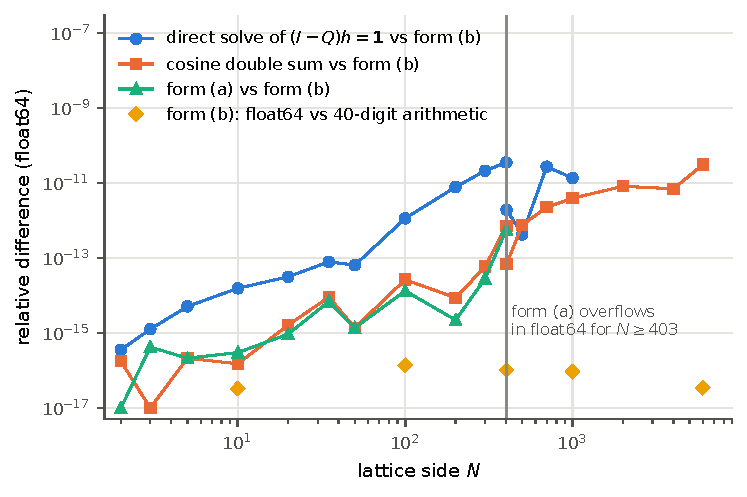
\includegraphics[width=0.74\textwidth]{s4_mfpt_verification.pdf}
\caption{Double-precision evaluation of $q\TN$ ($\dd=2$, corner to corner) by different routes, as relative
difference from form (b) of Theorem~\ref{s4_mfpt:thm-single}: sparse solve of $(I-\Qm)h=\one$ at $q=0.8$
(direct factorisation up to $N=300$, conjugate gradients from $N=402$, up to $N=1000$), cosine double
sum \eqref{s4_mfpt:eq-cosine-cc} (up to $N=6000$), and form (a), which is not finite for $N\ge403$
(vertical line). Diamonds: form (b) in double precision against 40-digit arithmetic. Differences that are
exactly zero are drawn at $10^{-17}$. The growth of the first two curves is rounding in the linear solve and
in the $\Order(N^{2})$-term sum, not in form (b).}
% src: data/msc_proof/verify_float.csv; data/msc_proof_verify/v5_extra.json;
% src: figure generated by code/article/s4_mfpt_figures.py
\label{s4_mfpt:fig-verif}
\end{figure}

\emph{Arbitrary pairs.} A second implementation confirms \eqref{s4_mfpt:eq-pair} to $1.7\times10^{-40}$ on 1956
cases (the 1848 ordered pairs with $N\le5$ at two values of $q$ and 108 random pairs with $6\le N\le17$).
% src: data/msc_proof_verify/v1_exact.json (pairs_exhaustive, pairs_random)
In double precision, with the hyperbolic ratios written through decaying exponentials, the formula reproduces a sparse
direct solve for every start site at $N=35$, $q=0.8$, to $7.9\times10^{-14}$ for the two targets of
Fig.~\ref{s4_mfpt:fig-landscape} and to $8.6\times10^{-14}$ in the second implementation (three targets).
% src: data/article/s4_mfpt_landscape_check.json; data/msc_proof/landscape_check.json;
% src: data/msc_proof_verify/v5_extra.json (thm3_float64_all_starts_N35_q0.8_worst_rel)
Numerically, $q\TN=2N^{2}\Reff_N$ holds to $1.2\times10^{-14}$ for $N=2,\dots,20$ when $\Reff_N$ is computed from the
pseudo-inverse of the grid Laplacian, and Eq.~(57) of \citet{TanTan2020} agrees with the pseudo-inverse of the grid
Laplacian to $4.3\times10^{-15}$ for all 4536 ordered pairs with $N\le7$. The one-directional time of
Theorem~\ref{s4_mfpt:thm-pair} needs, besides the resistance, the potential of a single node; \citet{TanTan2020} give a
single sum for the node potentials as well, which we have not compared.
% src: data/msc_proof_verify/v2_identities.json (corollary5); data/article/s4_mfpt_literature_check.json (eq57_vs_laplacian_pinv)

\begin{figure}[htb]
\centering
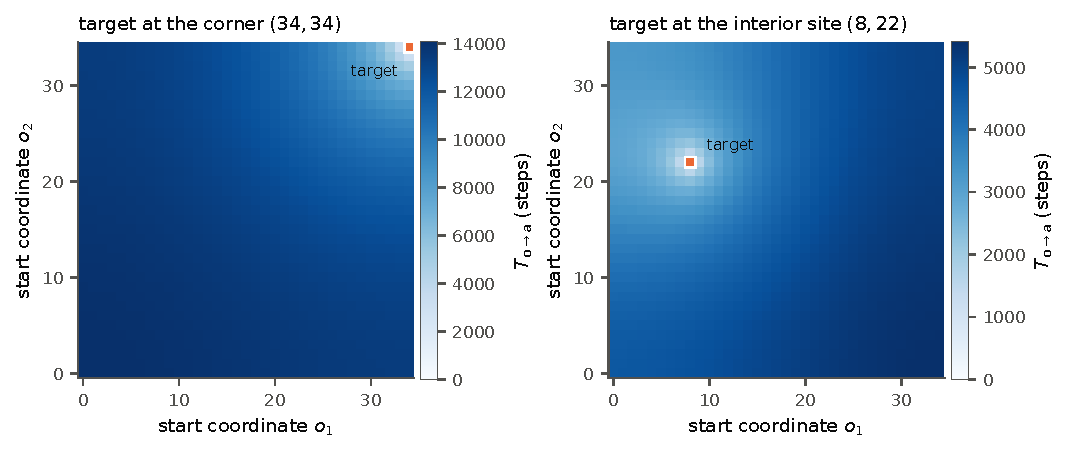
\includegraphics[width=0.86\textwidth]{s4_mfpt_landscape.pdf}
\caption{Mean first-passage time $\MF_{\vo\to\va}$ (steps) from every start site $\vo=(o_1,o_2)$ to a fixed
target $\va$ (square marker), computed with the single sum \eqref{s4_mfpt:eq-pair}; $\dd=2$, $N=35$, $q=0.8$,
discrete time, zero-based coordinates. Left: corner target $(34,34)$; the value at $(0,0)$ is
$\TN=14\,100.81$. Right: interior target $(8,22)$.}
% src: data/article/s4_mfpt_landscape_check.json (T_from_corner_00 = 14100.80804991771);
% src: figure generated by code/article/s4_mfpt_figures.py
\label{s4_mfpt:fig-landscape}
\end{figure}

\subsection{The expansion in numbers}

\begin{table}[htb]
\centering\small
\caption{Relative error of the expansion \eqref{s4_mfpt:eq-expansion} truncated after the stated number of
terms (two terms: $(8/\pi)N^{2}\ln N+C_{2}N^{2}$; five terms: up to $C_{-4}N^{-4}$), against the exact $q\TN$.}
\label{s4_mfpt:tab-trunc}
% src: data/msc_proof/asymptotic_truncation_errors.csv (columns 1-5 terms);
% src: data/msc_proof_verify/v3_asymptotics.json (truncation_table: same values);
% src: data/article/s4_mfpt_checks.json (truncation: re-computation with separately written code)
\begin{tabular}{@{}rccccc@{}}
\toprule
$N$ & 1 term & 2 terms & 3 terms & 4 terms & 5 terms\\
\midrule
10   & $2.7\times10^{-2}$ & $8.7\times10^{-4}$ & $1.7\times10^{-5}$  & $3.5\times10^{-7}$  & $2.2\times10^{-8}$ \\
35   & $1.7\times10^{-2}$ & $4.7\times10^{-5}$ & $7.7\times10^{-8}$  & $1.3\times10^{-10}$ & $6.7\times10^{-13}$\\
100  & $1.3\times10^{-2}$ & $4.5\times10^{-6}$ & $9.0\times10^{-10}$ & $1.9\times10^{-13}$ & $1.2\times10^{-16}$\\
1000 & $8.7\times10^{-3}$ & $3.0\times10^{-8}$ & $6.0\times10^{-14}$ & $1.3\times10^{-19}$ & $7.9\times10^{-25}$\\
4001 & $7.3\times10^{-3}$ & $1.6\times10^{-9}$ & $2.0\times10^{-16}$ & $2.6\times10^{-23}$ & $1.0\times10^{-29}$\\
\bottomrule
\end{tabular}
\end{table}

Table~\ref{s4_mfpt:tab-trunc} and Fig.~\ref{s4_mfpt:fig-asym} give the truncation errors. When terms in $N\ln N$ and in
odd powers of $N$ are admitted in the blind solve of Table~\ref{s4_mfpt:tab-coeff}, column (ii), the coefficients
found for $N\ln N$ and $N$ are below $10^{-28}$, and a free leading coefficient returns $8/\pi$ to $3\times10^{-58}$; for
the odd sizes $N=3^{j}$, $3\le j\le10$, the two forbidden coefficients are below $2\times10^{-15}$.
% src: data/msc_proof_verify/v3_asymptotics.json (forbidden_terms_2^j, forbidden_terms_3^j, leading_coefficient_minus_8/pi)
The coefficients grow quickly (the same solve gives $C_{-10}\approx-1685.5$), which suggests that the series is
asymptotic rather than convergent; we have not proved this.
% src: data/msc_proof_verify/v3_asymptotics.json (blind_even_power_fit, power -10)
By Theorem~\ref{s4_mfpt:thm-expansion}, $r_N=C_{0}+C_{-2}N^{-2}+\Order(N^{-4})$ with $C_{-2}<0$, so the remainder of
Theorem~\ref{s4_mfpt:thm-remainder} approaches $C_{0}$ from below, as the certified finite range shows; the limit
$r_N\to C_{0}$ is also proved, by a different route that evaluates $C_0$ as a series, in \Sref{R2}{Thm 9.8}.

\begin{figure}[htb]
\centering
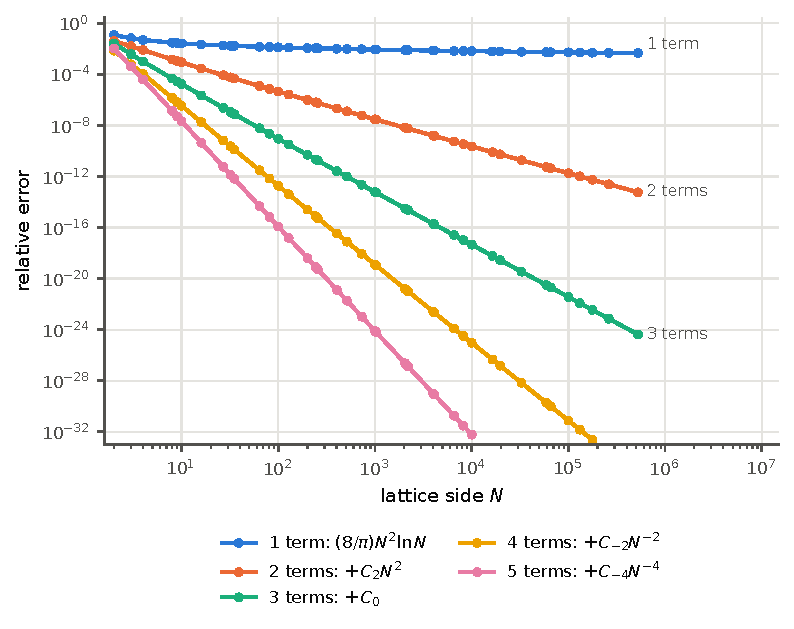
\includegraphics[width=0.78\textwidth]{s4_mfpt_asymptotics.pdf}
\caption{Relative error of the expansion \eqref{s4_mfpt:eq-expansion} truncated after one to five terms,
against exact values of $q\TN$ computed with form (b) to 50 digits ($\dd=2$, corner to corner; $N=2^{j}$, $3^{j}$,
$10^{j}$ and a few other sizes up to $N=524\,288$). Curves end where the error reaches the precision of the stored
values.}
% src: data/msc_proof/asymptotics.csv (exact values); data/article/s4_mfpt_truncation_errors.csv (plotted data);
% src: figure generated by code/article/s4_mfpt_figures.py
\label{s4_mfpt:fig-asym}
\end{figure}

\subsection{Three dimensions}\label{sup_mfpt:ssec-3d}

In double precision \eqref{s4_mfpt:eq-3d} agrees with sparse solves of $(I-\Qm)h=\one$ to $5.4\times10^{-13}$ or better
at the sizes tested ($N=3$, $5$, $8$, $12$).
% src: data/article/closed_form_checks.json (d3_corner: N = 3, 5, 8, 12, worst 5.409e-13); data/article/s4_mfpt_checks.json (three_dimensions.double_sum_vs_direct: N = 2, 3, 5, 8, 12, <= 4.0e-13)
Richardson extrapolation of the exact values gives $4.3204601701$ and $-3.887257$ for the first two constants of
Theorem~\ref{s4_mfpt:thm-3d}, and the remainder $q\TNd{3}-\Kthree N^{3}-\Kthreep N^{2}$ equals $1.44$, $1.457$ and
$1.458$ at $N=10$, $35$ and $100$, in agreement with the limit $\Kthree''$; beyond $N\approx400$ a ten-digit value of
$\Kthree$ does not resolve the remainder.
% src: data/msc_modes_verify/extra.json (C3_numeric_richardson, C3prime_numeric_richardson); data/article/s4_mfpt_checks.json (three_dimensions.large_N.remainder_after_two_terms)
In Theorem~\ref{s4_mfpt:thm-3d}, $\Ginf$ is $2\dd=6$ times the Green's function of the unit-conductance lattice
Laplacian, the normalisation of $\Glap$ elsewhere in this article. The identity for $\Kthree$ is elementary
(Section~\ref{appD_rigorous:sec}); the enclosure, the bounds on $R(N)$ and the values of $\Kthreep$ and $\Kthree''$ rest
on ball arithmetic. In Observation~\ref{s4_mfpt:obs-3d}, $\theta_{3}(x)=\sum_{n\in\mathbb Z}x^{n^{2}}$ and
$\theta_{4}(x)=\sum_{n\in\mathbb Z}(-1)^{n}x^{n^{2}}$ are theta functions of the nome $x$, and the observation gives
$\Kthreep=-\frac6\pi\,\xiH+\frac6{\pi^{2}}\,\varkappa$ to the precision stated. The constant $\xiH$ is not ours: it is the
lattice constant of the periodic simple-cubic lattice that appears in the periodic fundamental solution of
\citet{Hasimoto1959} and, with the value $2.837297$, in the finite-size correction of diffusion coefficients in
periodic boxes \citep{YehHummer2004}; the integral above is the representation we used to evaluate it.

% sup_modes.tex -- Supplementary Section S6: exact modes -- proofs for one dimension, further values, figures and fits.
% Numbers: code/article/s5_modes_tables.py -> data/article/s5_modes_tables.json;
% figures: code/article/s5_modes_figures.py, code/article/s3s6_modes_figures.py.
\section{Exact modes: proofs, further values and fits}\label{sup_modes:sec}

\subsection{Proofs for one dimension}\label{sup_modes:ssec-1d-proofs}

\begin{proof}[Proof of Proposition~\ref{s5_modes:prop-1d}]
Let $K$ be the $(N-1)\times(N-1)$ matrix of the $q=1$ chain restricted to the sites $0,\dots,N-2$:
$K(j,j\pm1)=\tfrac12$ whenever both indices lie in $\{0,\dots,N-2\}$, $K(0,0)=\tfrac12$ (the cancelled move at the
reflecting end), and zero otherwise; the move from $N-2$ to the target is not part of $K$. Then $\Qm=(1-q)I+qK$,
the vector of one-step absorption probabilities is $r=(q/2)\,\ve_{N-2}$, and $\pmf(t)=\ve_{0}^{\T}\Qm^{t-1}r$ by
\eqref{s2_model:eq-pmf}. Let $v_m(j)=\cos\bigl(\omega_m(j+\tfrac12)\bigr)$ for every integer $j$. The addition
formula gives $\tfrac12[v_m(j-1)+v_m(j+1)]=\cos\omega_m\,v_m(j)$ for all $j$. Since $v_m(-1)=v_m(0)$, the left-hand
side equals $(Kv_m)(0)$ at $j=0$; since $v_m(N-1)=\cos\bigl((2m-1)\pi/2\bigr)=0$, it equals $(Kv_m)(N-2)$ at
$j=N-2$. Hence $Kv_m=\cos\omega_m\,v_m$ on $\{0,\dots,N-2\}$ for $m=1,\dots,N-1$. The $\omega_m$ are distinct
points of $(0,\pi)$, so these are $N-1$ distinct eigenvalues of the symmetric matrix $K$ and the $v_m$ form an
orthogonal basis. Their norms follow from $\sum_{j=0}^{n-1}\cos\bigl((2j+1)\omega\bigr)=\sin(2n\omega)/(2\sin\omega)$
with $n=N-1$ and $2(N-1)\omega_m=(2m-1)\pi-\omega_m$:
\[
  \|v_m\|^{2}=\frac{N-1}{2}+\frac{\sin\bigl(2(N-1)\omega_m\bigr)}{4\sin\omega_m}=\frac{2N-1}{4}.
\]
Expanding $\Qm^{t-1}$ in this basis,
$\pmf(t)=\frac q2\sum_m\lambda_m^{t-1}\,v_m(0)\,v_m(N-2)/\|v_m\|^{2}$, with $v_m(0)=\cos(\omega_m/2)$ and
$v_m(N-2)=\cos\bigl((2m-1)\pi/2-\omega_m\bigr)=(-1)^{m+1}\sin\omega_m$, which is \eqref{s5_modes:eq-1d-pmf}.
For the mean, $h(j)=[N(N-1)-j(j+1)]/q$ satisfies $h(N-1)=0$ and
$\tfrac q2[2h(j)-h(j-1)-h(j+1)]=1$ for $0\le j\le N-2$, with $h(-1):=h(0)$; these are the equations that
characterise the mean hitting time in Proposition~\ref{s2_model:prop-pinv}, so $\MF=h(0)=N(N-1)/q$, in agreement
with Theorem~\ref{s4_mfpt:thm-cosine}.
\end{proof}

Equation~\eqref{s5_modes:eq-1d-pmf} agrees with explicit powers of $\Qm$ to $4.2\times10^{-17}$ in absolute value
($N=5,8,20,50$; $q=0.3,0.8,1$) and gives the same maximiser as time stepping at every size compared.
% src: data/article/s5_modes_tables.json (prop_1d_checks, modes_1d_closed_form); data/article/closed_form_checks.json (d1_closed_form_pmf); data/msc_modes/discrete_modes.jsonl (closed_form_max_abs_diff_window)

\begin{proof}[Proof of Proposition~\ref{s5_modes:prop-1d-limit}]
\emph{Rescaling.} By Proposition~\ref{s5_modes:prop-1d} and \eqref{s2_model:eq-spectral} the unit-rate density is
$\gd(t)=\sum_m b_m\eu^{-\nu_mt}$ with $\nu_m=1-\cos\omega_m$ and
$b_m=\ell^{-1}(-1)^{m+1}\cos(\omega_m/2)\sin\omega_m$. Put $\Phi_N(\xi)=2\ell^{2}\,\gd(2\ell^{2}\xi)
=\sum_{m=1}^{N-1}c_{N,m}\,\eu^{-a_{N,m}\xi}$ with $c_{N,m}=2\ell\,(-1)^{m+1}\cos(\omega_m/2)\sin\omega_m$ and
$a_{N,m}=2\ell^{2}(1-\cos\omega_m)$. For fixed $m$, $c_{N,m}\to(-1)^{m+1}(2m-1)\pi$ and
$a_{N,m}\to(2m-1)^{2}\pi^{2}/4$. Since $|\sin\omega|\le\omega$ and $1-\cos\omega\ge2\omega^{2}/\pi^{2}$ on
$[0,\pi]$, we have $|c_{N,m}|\le(2m-1)\pi$ and $a_{N,m}\ge(2m-1)^{2}$ for all $N$ and $m$, so the $m$-th term is
bounded by $(2m-1)\pi\,\eu^{-(2m-1)^{2}\xi_0}$ on $[\xi_0,\infty)$, uniformly in $N$. Each term converges
uniformly on $[\xi_0,\infty)$, and the bounds are summable; hence $\Phi_N\to\Phi$ uniformly on $[\xi_0,\infty)$
for every $\xi_0>0$.

(a) Each $\Phi_N$ is log-concave (Proposition~\ref{s3_methods:prop-1d-unimodal}(i)), and the inequality
$\Phi_N(\lambda\xi+(1-\lambda)\xi')\ge\Phi_N(\xi)^{\lambda}\Phi_N(\xi')^{1-\lambda}$ passes to the pointwise limit,
so $\Phi$ is log-concave. The series \eqref{s5_modes:eq-1d-continuum} converges uniformly on compact subsets of
$\{\operatorname{Re}\xi>0\}$, so $\Phi$ is analytic. For $\xi\ge0.05$ the moduli of the terms decrease from the
second term on, so consecutive partial sums bracket $\Phi$:
$\Phi(0.05)\le\pi\,(\eu^{-\pi^{2}/80}-3\,\eu^{-9\pi^{2}/80}+5\,\eu^{-25\pi^{2}/80})<0.40$,
$\Phi(\tfrac16)\ge\pi\,(\eu^{-\pi^{2}/24}-3\,\eu^{-9\pi^{2}/24})>1.84$ and
$\Phi(\tfrac12)\le\pi\,\eu^{-\pi^{2}/8}<0.92$.
% src: data/article/derived_checks.json (I_continuum_density_bounds)
For $\xi<0.05$ write $0.05=\lambda\xi+(1-\lambda)\tfrac16$ with $0<\lambda<1$; log-concavity gives
$\Phi(0.05)\ge\Phi(\xi)^{\lambda}\Phi(\tfrac16)^{1-\lambda}\ge\Phi(\xi)^{\lambda}\Phi(0.05)^{1-\lambda}$, hence
$\Phi(\xi)\le\Phi(0.05)<\Phi(\tfrac16)$ (if $\Phi(0.05)=0$ the first inequality gives $\Phi(\xi)=0$); in the same
way $\Phi(\xi)\le\Phi(\tfrac12)<\Phi(\tfrac16)$ for $\xi>\tfrac12$. Hence $\Phi$ attains its
supremum on $[0.05,0.5]$, and not at the end points. The set of maximisers of a log-concave function is an interval,
and an analytic function that is constant on an interval is constant; $\Phi$ is not constant, so the maximiser
$\xi^{*}$ is unique.

(b) Fix $\varepsilon>0$ with $[\xi^{*}-\varepsilon,\xi^{*}+\varepsilon]\subset(0,\infty)$. By (a),
$\Phi(\xi^{*}\pm\varepsilon)<\Phi(\xi^{*})$, so by the convergence just shown
$\Phi_N(\xi^{*}\pm\varepsilon)<\Phi_N(\xi^{*})$ for all large $N$. $\Phi_N$ is unimodal, so all its maximisers
then lie in $(\xi^{*}-\varepsilon,\xi^{*}+\varepsilon)$. The maximiser of $\gd$ is $\tmodec=2\ell^{2}\xi_N$ with
$\xi_N$ a maximiser of $\Phi_N$, and $q\MF=N(N-1)$; therefore $\tmodec/(q\MF)=2\xi_N\,\ell^{2}/(N(N-1))\to2\xi^{*}$.
At activity $q$ the mode is $\tmodec/q$ and the mean is $\MF$ (Proposition~\ref{s2_model:prop-structure}(d)), so
the ratio is the same.

(c) For $q\le\tfrac12$ all $\lambda_m=1-q\nu_m$ lie in $[0,1)$. With $t=2\ell^{2}\xi/q$,
\[
  \frac{2\ell^{2}}{q}\,\pmf(t)=\sum_{m=1}^{N-1}c_{N,m}\,\lambda_m^{\,t-1},\qquad
  0\le\lambda_m^{\,t-1}\le\eu^{-q\nu_m(t-1)}\le\eu^{2q}\,\eu^{-a_{N,m}\xi},
\]
because $\ln(1-x)\le-x$ and $\nu_m\le2$. For fixed $m$, $(t-1)\ln\lambda_m\to-(2m-1)^{2}\pi^{2}\xi/4$ uniformly for
$\xi$ in compact subsets of $(0,\infty)$, and the same domination as above gives
$(2\ell^{2}/q)\,\pmf(2\ell^{2}\xi/q)\to\Phi(\xi)$ uniformly on such subsets, for $\xi$ restricted to the values at
which $t$ is an integer. These values have spacing $q/(2\ell^{2})\to0$, so for large $N$ there are admissible
points $\xi_-<\xi_0<\xi_+$ in $(\xi^{*}-\varepsilon,\xi^{*}+\varepsilon)$ with $\xi_\pm$ within
$\varepsilon/2$ of $\xi^{*}\pm\varepsilon$ and $\xi_0$ so close to $\xi^{*}$ that the rescaled PMF is larger at
$\xi_0$ than at $\xi_\pm$ (the maximum of $\Phi$ over the two closed intervals of length $\varepsilon/2$ at the
ends is below $\Phi(\xi^{*})$). The PMF is unimodal on the integers
(Proposition~\ref{s3_methods:prop-1d-unimodal}(ii)), so every maximiser lies between $\xi_-$ and $\xi_+$, and
$\tmode/\MF=2\xi_N\,\ell^{2}/(N(N-1))\to2\xi^{*}$ as in (b).
\end{proof}

\begin{observation}[One dimension]\label{s5_modes:obs-1d}
At $q=0.8$ the four modes at $N=50$, $100$, $200$ and $1000$ quoted in Section~\ref{s5_modes:ssec-1d} are certified
global maximisers. At $N=10^{5}$ and $10^{6}$ the local maxima of \eqref{s5_modes:eq-1d-pmf} nearest the continuum
prediction are $4\,166\,011\,658$ and $416\,604\,915\,263$ (route~B); they equal $\lceil\tau\rceil$ of
Theorem~\ref{s6b_rigorous:thm-1d}(c), so they are the global maximisers.
% src: data/msc_modes_verify/bigN_1d_mp.json (field "recheck"); data/msc_modes/laplace_modes.jsonl (d = 1: mode_discrete_q0.8); data/article/s5_modes_tables.json (modes_1d_large_N, tab_modes_rows); data/article/s3_methods_certificate.jsonl (d = 1)
In continuous time $\tmodec/(q\MF)=0.3332842653$ at $N=3620$ and $0.33328426549$ at $N=10^{6}$, and
$\tmodec=0.33328427\,(N-\tfrac12)^{2}$, to the digits shown, at $N=10^{5}$ and $10^{6}$, in agreement with
Proposition~\ref{s5_modes:prop-1d-limit}(b).
% src: data/msc_modes/laplace_modes.jsonl (d = 1); data/msc_modes/summary_tables.md (M1); data/article/s5_modes_tables.json (lattice_ratio_1d_continuous_time)
\end{observation}

\subsection{Two and three dimensions: further values and figures}

At $q=0.8$ the exact two-dimensional modes are $\tmode=2493$, $22\,110$, $92\,116$ and $383\,013$ for $N=35$, $100$, $200$ and
$401$, and the three-dimensional ones $6644$, $8863$ and $62\,998$ for $N=35$, $40$ and $100$; all of them were
re-stepped once more with separately written code.
% src: data/msc_modes/tables.md (T2, T3); data/msc_modes/discrete_modes.jsonl; data/article/s5_modes_tables.json (stepper_recheck)
In two dimensions the ratio $\tmode/\MF$ is $0.2696$, $0.1768$, $0.1489$, $0.1350$ and $0.1236$ at $N=5$, $35$, $100$,
$200$ and $401$, and $0.0651$ and $0.0562$ at $N=1\,048\,576$ and $16\,777\,216$. In three dimensions it is
$4.2\times10^{-3}$ at $N=320$. In three dimensions the local exponent of the mode falls from $2.33$ ($N\approx6$) to $2.12$
($N\approx134$) and $2.085$ ($N\approx3200$), and the two continuous-time routes agree on the position of the maximum to
$1.1\times10^{-10}$, against $7\times10^{-13}$ in two dimensions.
% src: data/msc_modes/tables.md (T2); data/msc_modes/summary_tables.md (M2, M3); data/article/s5_modes_tables.json (tab_modes_rows, local_exponents); data/msc_modes_verify/analysis.json (summary_d2, summary_d3: max_rel_diff_mode_vs_talbot)

\begin{figure}[tbp]
\centering
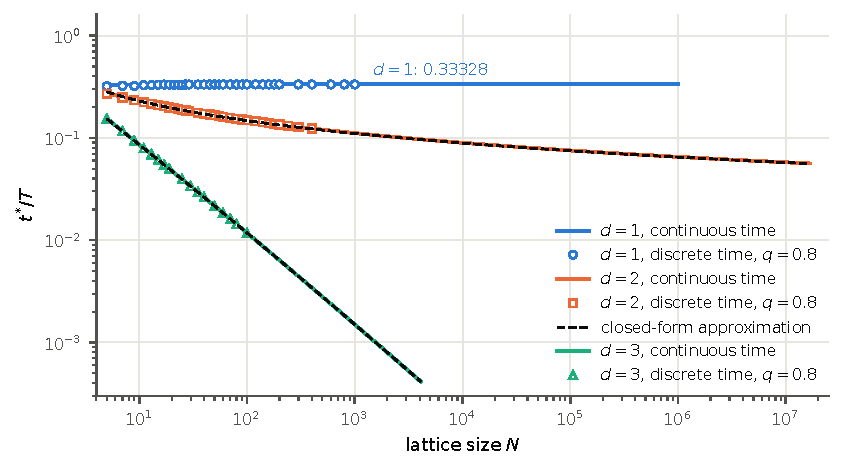
\includegraphics[width=0.92\textwidth]{s5_modes_ratio.pdf}
\caption{Mode-to-mean ratio $\tmode/\MF$ against lattice size, corner to opposite corner. Lines: exact
continuous-time values (independent of $q$). Symbols: exact discrete-time PMF at $q=0.8$. Dashed: closed-form
approximation \eqref{s6_mechanism:eq-L1}.}
% src: code/article/s5_modes_figures.py; data/msc_modes/laplace_modes.jsonl, discrete_modes.jsonl
\label{s5_modes:fig-ratio}
\end{figure}

\begin{figure}[tbp]
\centering
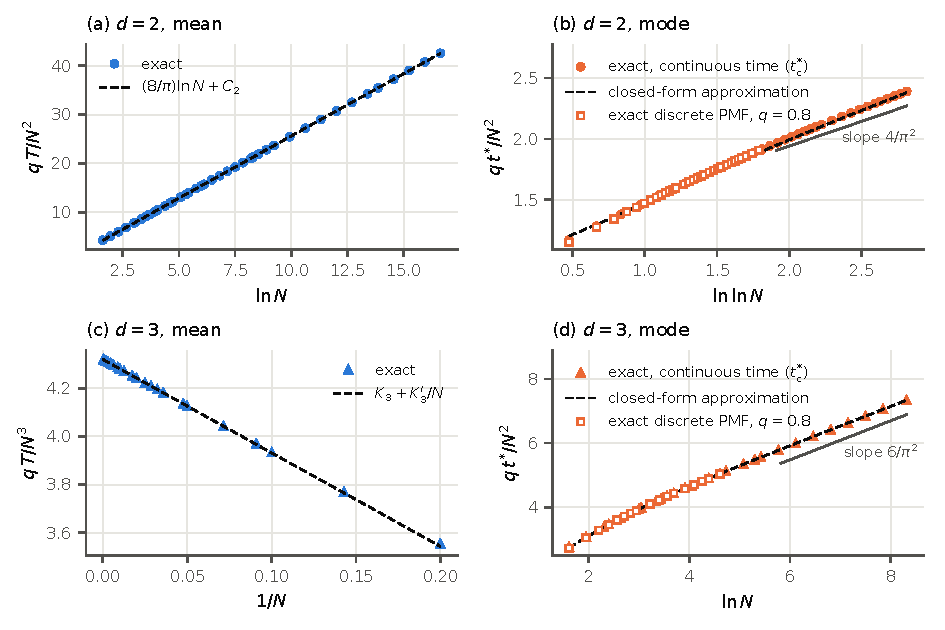
\includegraphics[width=\textwidth]{s5_modes_compensated.pdf}
\caption{Compensated plots, corner to opposite corner. (a) $\dd=2$: $q\MF/N^{2}$ against $\ln N$ with the two-term
law of Theorem~\ref{s4_mfpt:thm-expansion}. (b) $\dd=2$: $q\tmode/N^{2}$ against $\ln\ln N$. (c) $\dd=3$:
$q\MF/N^{3}$ against $1/N$ with $\Kthree+\Kthreep/N$. (d) $\dd=3$: $q\tmode/N^{2}$ against $\ln N$. Filled symbols:
exact continuous-time values; open squares: exact discrete-time PMF at $q=0.8$; dashed lines in (b) and (d): the
closed-form approximation \eqref{s6_mechanism:eq-L1}; grey segments: the slopes
$4/\pi^{2}$ and $6/\pi^{2}$ of the leading laws (Theorem~\ref{s6b_rigorous:thm-laws}).}
% src: code/article/s3s6_modes_figures.py; data/msc_modes/laplace_modes.jsonl, discrete_modes.jsonl, fit_results.json
\label{s5_modes:fig-compensated}
\end{figure}

\begin{figure}[tbp]
\centering
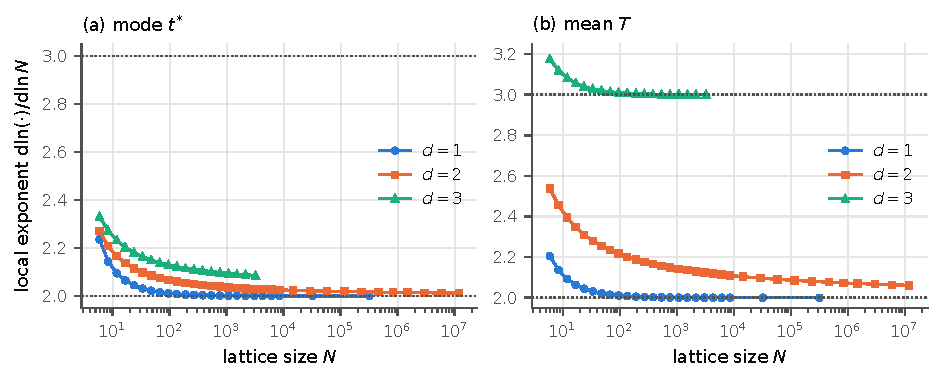
\includegraphics[width=\textwidth]{s5_modes_exponents.pdf}
\caption{Local exponents $\dif\ln(\cdot)/\dif\ln N$ of (a) the mode and (b) the mean, corner to opposite corner,
from exact continuous-time values at successive sizes (finite differences, plotted at the geometric mean of the two
sizes). The mode laws (Proposition~\ref{s5_modes:prop-1d-limit}, Theorem~\ref{s6b_rigorous:thm-laws}) give the limit
$2$ for the mode exponent in every dimension, approached slowly for $\dd=2,3$ because of the logarithmic factors.}
% src: code/article/s5_modes_figures.py; data/msc_modes/fit_results.json (effective_exponents)
\label{s5_modes:fig-exponents}
\end{figure}

\subsection{What scaling fits can and cannot show}\label{s5_modes:ssec-fits}

We record what least-squares fits over moderate ranges give when applied to the exact modes. The data are exact, so
the intervals quoted below are least-squares $95\%$ intervals computed from the residuals about each functional form:
they measure misfit, not noise, and are conditional on the form and on the window. For the exact discrete-time modes at
$q=0.8$, on the computed sizes in $10\le N\le200$ for $\dd=1,2$ (25 sizes each) and in $10\le N\le100$ for $\dd=3$ (14
sizes), the smallest of them being $N=11$, a pure power law $AN^{a}$ gives $a=2.031\pm0.006$ ($\dd=1$), $2.090\pm0.006$
($\dd=2$) and $2.169\pm0.009$ ($\dd=3$);
% src: data/msc_modes/tables.md (discrete short-range blocks, row P); data/msc_modes/fit_results.json (fits: *_mode_discrete_short_range)
none of these exponents is a property of the model, since each drifts with the window: for $\dd=2$ in continuous
time (13 sizes in the first window), $2.093\pm0.011$ on $10\le N\le200$, $2.033\pm0.004$ on $10\le N\le1.7\times10^{7}$ and $2.019\pm0.001$ on
$10^{3}\le N\le1.7\times10^{7}$.
% src: data/msc_modes/tables.md (2D mode fit blocks, row P); data/article/s5_modes_tables.json (tab_fits: power_law_exponent_2d_continuous_by_window)
Inside the fitting window the residuals do not single out the correct law: on the corrected Akaike criterion the
three-parameter form $AN^{a}(\ln N)^{b}$ is preferred to $N^{2}(A\ln\ln N+B)$ in every window examined, with a
fitted $a$ below $2$.
% src: data/msc_modes/tables.md (dAICc columns); data/article/s5_modes_tables.json (tab_fits: dAICc_lnln_form_minus_best_by_window_2d)
Extrapolation discriminates (Table~\ref{s5_modes:tab-fits}); the complete fits for $\dd=2,3$ are in
Table~\ref{appC_tables:tab-fits-full}, and those for $\dd=1$ in the file \texttt{data/msc\_modes/fit\_results.json} of the repository.

\begin{table}[tbp]
\centering
\caption{Least-squares fits of each form to $\ln\tmodec$ (exact continuous-time modes, unit rate) and their
extrapolation error, (prediction $-$ exact)/exact, at the largest computed size. Half-widths are $95\%$
least-squares intervals; on exact data they measure misfit, not noise. Last row of each block: closed-form
approximation \eqref{s6_mechanism:eq-L1}, no fitted parameter.}
% src (all rows): data/msc_modes/tables.md ("2D mode (continuous time, unit rate): fit on N = 10..200, extrapolated"; "3D mode ...: fit on N = 10..100, extrapolated"); data/msc_modes/fit_results.json (fits); closed form: data/msc_modes/laplace_modes.jsonl (pred_L1); data/article/s5_modes_tables.json (tab_fits)
\label{s5_modes:tab-fits}
\small
\begin{tabular}{@{}llcr@{}}
\toprule
model & fitted exponents or coefficients & rms $\ln$-residual & extrapolation error\\
\midrule
\multicolumn{4}{@{}l}{$\dd=2$: fitted on $10\le N\le200$ (13 sizes), evaluated at $N=16\,777\,216$}\\
$AN^{2}$ & -- & $8.3\times10^{-2}$ & $-30.8\%$\\
$AN^{a}$ & $a=2.093\pm0.011$ & $1.5\times10^{-2}$ & $+124.9\%$\\
$AN^{2}(\ln N)^{b}$ & $b=0.343\pm0.014$ & $5.2\times10^{-3}$ & $+15.0\%$\\
$AN^{a}(\ln N)^{b}$ & $a=1.953\pm0.004$, $b=0.515\pm0.014$ & $5.7\times10^{-4}$ & $-19.0\%$\\
$N^{2}(A\ln\ln N+B)$ & $A=0.555\pm0.007$, $B=0.922\pm0.009$ & $1.6\times10^{-3}$ & $+3.8\%$\\
approximation \eqref{s6_mechanism:eq-L1} & -- & -- & $-0.45\%$\\
\midrule
\multicolumn{4}{@{}l}{$\dd=3$: fitted on $10\le N\le100$ (10 sizes), evaluated at $N=4096$}\\
$AN^{3}$ & -- & $5.8\times10^{-1}$ & $+6799\%$\\
$AN^{2}$ & -- & $1.2\times10^{-1}$ & $-41.6\%$\\
$AN^{a}$ & $a=2.170\pm0.014$ & $1.2\times10^{-2}$ & $+31.7\%$\\
$AN^{2}(\ln N)^{b}$ & $b=0.572\pm0.002$ & $4.9\times10^{-4}$ & $-3.8\%$\\
$AN^{a}(\ln N)^{b}$ & $a=2.006\pm0.003$, $b=0.553\pm0.011$ & $2.6\times10^{-4}$ & $-2.7\%$\\
$N^{2}(A\ln N+B)$ & $A=0.721\pm0.023$, $B=1.76\pm0.08$ & $4.9\times10^{-3}$ & $+5.7\%$\\
approximation \eqref{s6_mechanism:eq-L1} & -- & -- & $+6.0\times10^{-7}$\\
\bottomrule
\end{tabular}
\end{table}

% sup_mechanism.tex -- Supplementary Section S7: the factorisation, the ingredients of the closed form, accuracy
% figure, shape in discrete time, and other placements.  Tables: code/article/s6_mechanism_tables.py;
% figures: code/article/s3s6_modes_figures.py.
\section{Pole structure and shape: proofs and further results}\label{sup_mechanism:sec}

\subsection{Proof of Proposition~\ref{s6_mechanism:prop-factorisation}}

By \eqref{s2_model:eq-renewal} the first-passage transform from a start $\vx\neq\va$ is
$\Phat(\va,s\,|\,\vx)/\Phat(\va,s\,|\,\va)$, and the same expression equals $1$ for $\vx=\va$, in agreement with
$\FPT_{\mathrm u}=0$ there. Averaging over $\vx$ gives
$\Fhat_{\mathrm u}(s)=\nn^{-1}\sum_{\vx}\Phat(\va,s\,|\,\vx)/\Phat(\va,s\,|\,\va)$. Since $\Pm$ is symmetric,
$\sum_{\vx}p(\va,t\,|\,\vx)=\sum_{\vx}p(\vx,t\,|\,\va)=1$ for all $t$, hence $\sum_{\vx}\Phat(\va,s\,|\,\vx)=1/s$; this is the
first identity. The second follows because $s\,\hat u(s)\,\Fhat_{\mathrm u}(s)=\Phat(\va,s\,|\,\vo)/\Phat(\va,s\,|\,\va)$. As
$u(0)=\nn\,\delta_{\vo\va}=0$, $s\hat u(s)$ is the transform of $u'$, and a product of transforms is the transform of a
convolution. For \eqref{s6_mechanism:eq-u}: at unit rate the $\dd$ coordinates are independent one-dimensional walks of
rate $1/\dd$ (Lemma~\ref{appA_proofs:lem-spectrum}), so $p$ is a product of one-dimensional propagators
$\sum_k\psi_k(m)\psi_k(m')\eu^{-\varepsilon_k t}$, and $\psi_k(N-1)\psi_k(0)=(\alk{k}/N)(-1)^{k}\ck{k}^{2}$ because
$\thk{k}{N-1}=\pi k-\thk{k}{0}$. Finally $\varepsilon_k/\muone=\sk{k}^{2}/\sk{1}^{2}\to k^{2}$ and $\ck{k}\to1$ for fixed $k$,
while $\sk{k}\ge k/N$ and $\sk{1}\le\pi/(2N)$ give $\varepsilon_k/\muone\ge4k^{2}/\pi^{2}$ for all $1\le k\le N-1$; the
$k$-th term is therefore bounded by $2\eu^{-4k^{2}x/\pi^{2}}$ uniformly in $N$, and dominated convergence gives the
limit. \hfill$\square$
% src: data/article/s6_mechanism_tables.json (factorisation_check: identities reproduced by dense linear algebra to 3.5e-14 on four small lattices, d = 2, 3; arrival_profile_convergence: max |u - theta_4^d| on 0.05 <= x <= 12 is 1.3e-2, 1.3e-4, 1.3e-6 at N = 10, 100, 1000, d = 2)

Numerically the two identities \eqref{s6_mechanism:eq-factor} are reproduced by dense linear algebra to
$3.5\times10^{-14}$ on four small lattices ($\dd=2,3$), and $\max|u(x/\muone)-\theta_4(\eu^{-x})^{2}|$ on
$0.05\le x\le12$ is $1.3\times10^{-2}$, $1.3\times10^{-4}$ and $1.3\times10^{-6}$ at $N=10$, $100$ and $1000$ ($\dd=2$).

\subsection{The ingredients of the closed form}\label{sup_mechanism:ssec-ingredients}

In \eqref{s6_mechanism:eq-poles} the two smallest zeros $\nu_{(0)}$, $\nu_{(1)}$ of
Proposition~\ref{s2_model:prop-interlacing} are written $\nu_0$, $\nu_1$, which is consistent with
\eqref{s2_model:eq-spectral} whenever both residues are non-zero, as they are for the corner start. The two zero
conditions are $1/\nu_0=W/(\mu-\nu_0)+R(-\nu_0)$ and $W/(\nu_1-\mu)=R(-\nu_1)-1/\nu_1$, and the residues are dominated
by the terms in $1/s$ at $-\nu_0$ and by the terms in $1/(s+\mu)$ at $-\nu_1$.

Equation~\eqref{s6_mechanism:eq-L1} corrects the rate difference but not $\nu_0\,q\MF$, the ratio $b_1/b_0$ or the
argument of the logarithm, and the omitted terms partly cancel. At $\dd=2$, $N=100$, replacing the exact argument
$-b_1\nu_1/b_0\nu_0$ by $AX$ lowers the prediction by $2.5\%$, the first-order rate difference raises it by $1.1\%$ and
the neglect of the poles $j\ge2$ raises it by $0.4\%$; the net error is $-0.97\%$.
% src: data/article/s6_mechanism_tables.json (ingredients/2d_CC, N = 100: factor_log 0.97535, factor_rate 1.01128, factor_third_pole 1.00401)
The ingredients can also be checked one by one against the numerically exact poles: $\nu_0\,q\MF$ falls from $1.164$
($N=5$) to $1.021$ ($N=16\,777\,216$) for $\dd=2$ and from $1.076$ to $1.0001$ ($N=4096$) for $\dd=3$; $(\nu_1/\muone-1)X/W$
goes from $1.15$ to $1.036$ and from $0.911$ to $0.9998$; and $b_1/b_0$ reaches $-4.087$ and $-5.9994$ at the largest
sizes, against $-A=-4$ and $-6$.
% src: data/article/s6_mechanism_tables.json (ingredients; from data/msc_modes/laplace_modes.jsonl); data/msc_modes/fit_results.json (pole_structure)
The maximum sits where the two regimes of Fig.~\ref{s6_mechanism:fig-density} meet: $\nu_1\tmodec$ is $4.81$ to $6.13$ for
$\dd=2$ ($N=35$ to $16\,777\,216$) and $7.44$ to $12.07$ for $\dd=3$ ($N=40$ to $4096$), against $\ln(2\dd X)=4.51$ to $6.04$
and $7.42$ to $12.07$.
% src: data/article/s6_mechanism_tables.json (ingredients: nu1_tmode, ln_2dX)

\emph{Accuracy.} The leading-order form \eqref{s6_mechanism:eq-L0} errs by $+7.3\%$ at $N=10$ and $+0.017\%$ at $N=4096$
for $\dd=3$; the closed-form approximation \eqref{s6_mechanism:eq-L1} is within $2.6\times10^{-4}$ for $N\ge35$ in three dimensions, and
below $N=10$ the errors are larger ($+2.7\%$ at $N=5$ for $\dd=2$). The exact two-exponential truncation is within
$0.66\%$ ($\dd=2$) and $0.15\%$ ($\dd=3$), with an error of the opposite sign to that of \eqref{s6_mechanism:eq-L1}, and
the exact three-exponential truncation reaches $1.4\times10^{-8}$ at $N=16\,777\,216$ (Fig.~\ref{s6_mechanism:fig-accuracy}).
% src: data/article/closed_form_checks.json (3d_CC: L0, L1_weights); data/msc_modes/summary_tables.md (M2); data/article/s6_mechanism_tables.json (accuracy/2d_CC/rows; accuracy: two_pole, three_pole); data/msc_modes/tables.md (accuracy lines)
In discrete time the error of \eqref{s6_mechanism:eq-L1-simple} is certified on finite ranges: at most $0.970\%$ for
$\dd=2$ ($q=0.8$, $10\le N\le301$ and five larger sizes) and $0.275\%$ for $\dd=3$ ($q=0.8$, $10\le N\le120$ and four larger
sizes), and for $\dd=3$ it stays below $0.3\%$ for every $N\ge10$ (Theorem~\ref{s6b_rigorous:thm-cffinite} and
Corollary~\ref{s6b_rigorous:cor-cf}).
% src: data/msc_rigorous_certified/closedform_summary_c128.json (d2_q4-5, d3_q4-5: eps[10,...]); data/article/s6b_rigorous_checks.json (continuous_time_against_windows; corollary_closed_form_all_N)

\begin{figure}[tbp]
\centering
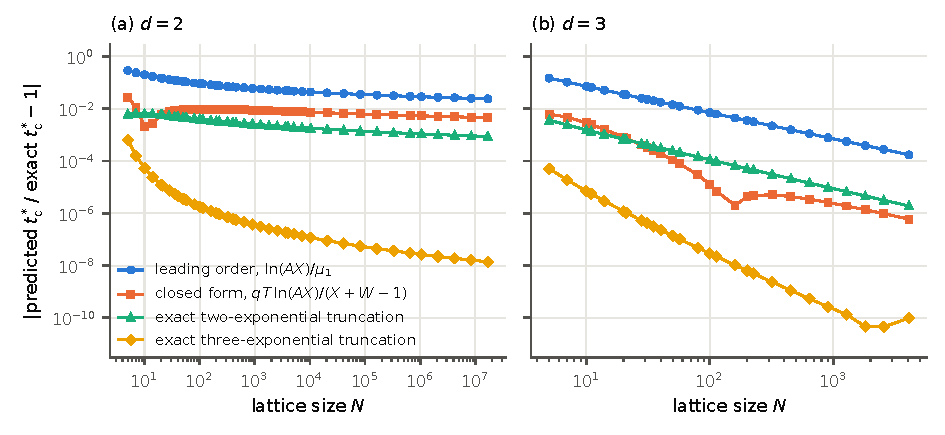
\includegraphics[width=\textwidth]{s6_mechanism_accuracy.pdf}
\caption{Absolute relative error of the predicted continuous-time mode (unit rate), corner to corner, against
the lattice size: (a) $\dd=2$, 43 sizes, $5\le N\le16\,777\,216$; (b) $\dd=3$, 27 sizes, $5\le N\le4096$.
Circles: leading order \eqref{s6_mechanism:eq-L0}; squares: closed-form approximation \eqref{s6_mechanism:eq-L1}
(for these placements $A=W$); triangles and diamonds: exact two- and three-exponential truncations. Dips of the
closed-form curves mark sign changes of the error. The three-exponential curve in (b)
levels off near $10^{-10}$, the accuracy to which the reference modes are known for $\dd=3$.}
\label{s6_mechanism:fig-accuracy}
% src: code/article/s3s6_modes_figures.py; data data/msc_modes/laplace_modes.jsonl
\end{figure}

\subsection{Shape in discrete time}

The shape statistics of Table~\ref{s6_mechanism:tab-shape} are found in discrete time at $q=0.8$ as well, from
distributions summed over their whole support ($\Prob(\FPT\le\tmode)=0.0981$, median $10\,145$ steps against
$\MF=14\,100.8$ for $\dd=2$, $N=35$), where the coefficient of variation is $0.816$ ($\dd=1$; the continuum value is
$\sqrt{2/3}$), $0.918$ ($\dd=2$, $N=35$) and $0.976$ ($\dd=3$, $N=15$), increasing towards the value 1 of an exponential law.
% src: data/msc_modes/full_tail.json; data/msc_modes/summary_tables.md (U); data/msc_modes_verify/constants.json (1d_cv)
The density at its maximum is within $5.5\%$ ($\dd=2$, $N=35$) and $1.2\%$ ($\dd=3$, $N=40$) of $1/\MF$, and for $\dd=3$ it
stays within $1\%$ of its maximum from $0.62$ to $5.6$ modal times at $N=640$. In the variable $x=\muone t$ the density
follows $\theta_4(\eu^{-x})^{\dd}$ closely for $\dd=3$ and converges slowly for $\dd=2$, as expected when the corrections are
of order $1/X$.
% src: data/msc_modes/medians.json; data/article/s6_mechanism_tables.json (shape_table); data/msc_modes/profile_stats.json (d = 3, N = 640: t_lo_0.99/mode = 0.616, t_hi_0.99/mode = 5.570)

\subsection{Other placements and extended targets}\label{sup_mechanism:ssec-geometries}

\begin{table}[tbp]
\centering
\caption{Other placements. (a) Point targets, continuous time at unit rate: corner start and centre target
(\CtM) and centre start and corner target (\MtC), odd $N$; the last column is the signed error of
\eqref{s6_mechanism:eq-L1}, which does not apply to \MtC{} ($A=0$, $b_1>0$). (b) Exit from the centre through
an absorbing boundary layer (\EXIT): continuum limit of $\tmode/\MF$ and exact lattice value at $q=0.8$
(discrete time).}
\label{s6_mechanism:tab-geometries}
% src: data/article/s6_mechanism_rows.tex, s6_mechanism_tables.json (geometries), from data/msc_modes/laplace_modes.jsonl (C2M, M2C), data/msc_modes/discrete_modes.jsonl (group exit), data/msc_modes/fit_results.json (continuum_exit); agrees with data/msc_modes/summary_tables.md (G) and data/msc_modes_verify/constants.json
\begin{tabular}{rlrcccc}
\toprule
\multicolumn{7}{l}{(a) point targets}\\
$\dd$ & placement & $N$ & $\tmodec/N^{2}$ & $\tmodec/q\MF$ & sign of $b_1$ & error of \eqref{s6_mechanism:eq-L1} (\%)\\
\midrule
2 & \CtM & 11 & 0.3838 & 0.19761 & $-$ & $-0.1930$ \\
2 & \CtM & 161 & 0.4694 & 0.12858 & $-$ & $-0.9491$ \\
2 & \CtM & 10\,241 & 0.5369 & 0.08529 & $-$ & $-0.7060$ \\
2 & \CtM & 655\,361 & 0.5779 & 0.06463 & $-$ & $-0.5307$ \\
2 & \MtC & 11 & 0.3122 & 0.05568 & $+$ & -- \\
2 & \MtC & 161 & 0.4504 & 0.03623 & $+$ & -- \\
2 & \MtC & 10\,241 & 0.5452 & 0.02370 & $+$ & -- \\
2 & \MtC & 655\,361 & 0.5990 & 0.01783 & $+$ & -- \\
3 & \CtM & 11 & 0.9446 & 0.06011 & $-$ & $+0.2055$ \\
3 & \CtM & 161 & 1.3894 & 0.00571 & $-$ & $+0.0021$ \\
3 & \CtM & 1281 & 1.7087 & 0.00088 & $-$ & $+0.0002$ \\
3 & \MtC & 11 & 0.7765 & 0.01827 & $+$ & -- \\
3 & \MtC & 161 & 1.3902 & 0.00201 & $+$ & -- \\
3 & \MtC & 1281 & 1.7779 & 0.00032 & $+$ & -- \\
\midrule
\multicolumn{7}{l}{(b) exit through an absorbing boundary}\\
$\dd$ & & $N$ & continuum $\tmode/\MF$ & lattice $\tmode/\MF$ & $\tmode$ (steps) & $\MF$ (steps)\\
\midrule
1 & \EXIT & 401 & 0.333284 & 0.33328 & 16\,664 & 50\,000.0 \\
2 & \EXIT & 201 & 0.474907 & 0.47489 & 6997 & 14\,734.0 \\
3 & \EXIT & 51 & 0.560839 & 0.56107 & 591 & 1053.3 \\
\bottomrule
\end{tabular}
\end{table}

\begin{figure}[tbp]
\centering
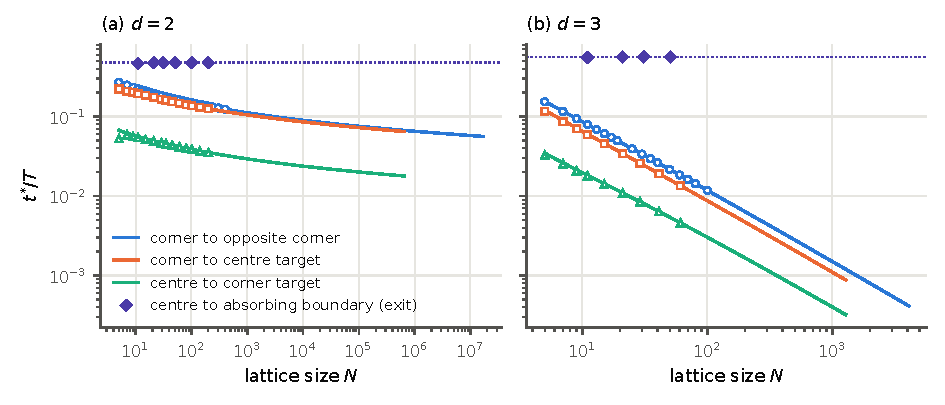
\includegraphics[width=\textwidth]{s6_mechanism_geometries.pdf}
\caption{Mode-to-mean ratio $\tmode/\MF$ against the lattice size for four placements, (a) $\dd=2$, (b) $\dd=3$.
Lines: continuous time; open symbols: exact discrete-time modes at $q=0.8$ (circles: corner to opposite corner;
squares: corner to centre; triangles: centre to corner). Diamonds: exit from the centre through an absorbing
boundary layer, discrete time, $q=0.8$; dotted line: its continuum limit, $0.474907$ ($\dd=2$) and $0.560839$
($\dd=3$).}
\label{s6_mechanism:fig-geometries}
% src: code/article/s3s6_modes_figures.py; data data/msc_modes/laplace_modes.jsonl, discrete_modes.jsonl, fit_results.json
\end{figure}

Table~\ref{s6_mechanism:tab-geometries} and Fig.~\ref{s6_mechanism:fig-geometries} show how far the results extend. For both
centre placements the law is unimodal (Theorem~\ref{s6b_rigorous:thm-unimodal}), but the mode laws are proved only for
corner-to-corner transport. A centre target reached from a corner behaves as the corner target does, with
$\mu\approx4\muone$. For a centre start and a corner target the density approaches its exponential tail from above, and
$\tmodec/N^{2}$ again grows slowly with $N$. Only these placements were examined.
% src: data/article/s6_mechanism_tables.json (c2m_weights_check: stored mu, W, A equal these expressions to round-off)

An extended target is different. If the walker starts at the centre and the whole boundary layer absorbs, there is no
small parameter: capture and relaxation happen on the same scale. In continuous time the coordinates are independent,
so the survival probability is the $\dd$-th power of that of a one-dimensional walk of rate $1/\dd$ between two absorbing
ends, and in the diffusive limit $\tmode/\MF$ tends to a constant: $0.333284$, $0.474907$ and $0.560839$ for $\dd=1,2,3$
(for $\dd=1$ this is the constant \eqref{s5_modes:eq-1d-ratio}, by symmetry about the centre). The lattice values at
$q=0.8$ agree with these constants to between three and five digits (Table~\ref{s6_mechanism:tab-geometries}b). For exit
the ratio therefore tends to a constant that grows with the dimension, whereas for a point target in $\dd\ge2$ it
decreases with $N$.
% src: data/msc_modes/fit_results.json (continuum_exit); data/msc_modes_verify/constants.json (0.3332842655, 0.4749066852, 0.5608388055); data/msc_modes/discrete_modes.jsonl (group exit)

The activity dependence is tabulated in Table~\ref{appC_tables:tab-activity}.

% appD_rigorous.tex -- Supplementary Section S8: proofs for Section 7 (s6b_rigorous) and for the computer-assisted
% results of Section 4.  Short proofs are given in full; for long and computer-assisted proofs the exact place of the
% complete proof in the companion notes (R0-R5, folder proofs/ of the repository) is given.  Notation of the article
% (zero-based sites).  Paths in "% src:" comments are relative to the root of the repository (see README.md).
\section{Proofs of the results on the mode}\label{appD_rigorous:sec}

This section gives the short proofs of Section~\ref{s6b_rigorous:sec} of the main text and of the computer-assisted
results of Section~\ref{s4_mfpt:sec}, and points to the place of every other proof in the companion notes R0--R5.

Throughout, $\Lm_1=I-\Pm_1$ is the unit-rate generator (with sign reversed) and, for real $s$ outside its spectrum,
\[
G(s)=\ve_{\va}^{\T}(\Lm_1-sI)^{-1}\ve_{\va}=\sum_{i}\frac{w_i}{\mu_{(i)}-s},\qquad
G_{\vx}(s)=\ve_{\vx}^{\T}(\Lm_1-sI)^{-1}\ve_{\va},
\]
with the visible reflecting rates $\mu_{(i)}$ and weights $w_i$ of Proposition~\ref{s2_model:prop-interlacing}, so
that $G(s)=\Phat(\va,-s\mid\va)$. Its zeros are the rates $\nu_{(i)}$, $G$ increases strictly between consecutive
poles, and the residues of the survival function from $\vx$ are $r_j(\vx)=-G_{\vx}(\nu_j)/(\nu_jG'(\nu_j))$
\Sref{R2}{Thm 3.1}.

\subsection{Two lemmas used by the certificates}

\begin{lemma}[Tail lemma]\label{appD_rigorous:lem-tail}
Let $v_t=\Qm^{\,t-1}\ve_{\vo}$ be the occupation probabilities of the surviving walker. If $v_{T+1}<v_T$ at every
site other than the target for some $T\ge1$, then $v_{t+1}<v_t$ and $\pmf(t+1)<\pmf(t)$ for all $t\ge T$. If moreover
$v_{T+1}\le\gamma v_T$ with $\gamma<1$, then $\pmf(T+s)\le\gamma^{s}\pmf(T)$ for $s\ge0$.
\textup{(Source: \Sref{R5}{Lemma 5}, \Sref{R4}{Lemma 6.1}.)}
\end{lemma}

\begin{proof}
$w_t=v_t-v_{t+1}$ satisfies $w_{t+1}=\Qm w_t$. Every row of $\Qm$ has a positive entry and $\Qm\ge0$, so
$w_T>0$ gives $w_t>0$ for $t\ge T$, and $\pmf(t)-\pmf(t+1)=r^{\T}w_t>0$ because $\pmf(t)=r^{\T}v_t$ by
\eqref{s2_model:eq-pmf} and $\Qm$ is symmetric. If $v_{T+1}\le\gamma v_T$, then
$v_{T+s+1}=\Qm^{s}v_{T+1}\le\gamma\Qm^{s}v_T=\gamma v_{T+s}$ entrywise, since $\Qm\ge0$.
\end{proof}

The exact certificates of R4 and R5 compute $v_t$ in integer arithmetic (after scaling $\Qm$ to an integer matrix)
until such a time $T$; Proposition~\ref{s3_methods:prop-certificate} is a coarser bound of the same kind.

\begin{lemma}[Rational enclosure of the mean]\label{appD_rigorous:lem-encl}
Let $h=(I-\Qm_1)^{-1}\one$ be the vector of unit-rate mean hitting times of $\va$. For every vector $z$ with
$R:=(I-\Qm_1)z>0$ entrywise, $z/\max R\le h\le z/\min R$ entrywise.
\textup{(Source: \Sref{R5}{Lemma 19}.)}
\end{lemma}

\begin{proof}
The spectral radius of $\Qm_1$ is below one (Section~\ref{s2_model:ssec-fp}), so
$(I-\Qm_1)^{-1}=\sum_{k\ge0}\Qm_1^{k}\ge0$ entrywise. Apply it to $z/\min R-h$, whose image
$R/\min R-\one$ is non-negative, and to $h-z/\max R$.
\end{proof}

A floating-point guess $z$ rounded to integers gives intervals of relative width below $10^{-28}$, which is how the
means behind Theorem~\ref{s6b_rigorous:thm-cffinite} are enclosed \Sref{R5}{Section 5}.

\subsection{Structure and signs (Section~\ref{s6b_rigorous:ssec-structure})}

\begin{proof}[Proof of Theorem~\ref{s6b_rigorous:thm-signs}]
(a) By Proposition~\ref{s2_model:prop-structure}, $\sum_jr_j\eu^{-\nu_jt}=\ve_{\vo}^{\T}\eu^{-(I-\Qm_1)t}\one$;
differentiating $i$ times at $t=0$ gives $\sum_jr_j\nu_j^{\,i}=\ve_{\vo}^{\T}(I-\Qm_1)^{i}\one
=\ve_{\vo}^{\T}(I-\Qm_1)^{i-1}r_1$ for $i\ge1$. The vector $r_1$ is supported on the neighbours of $\va$, which are
at distance at least $D-1$ from $\vo$, and the entry $(\vo,\vy)$ of $(I-\Qm_1)^{i-1}$ vanishes if $i-1<|\vo-\vy|_1$;
for $i=D$ only the term $(-\Qm_1)^{D-1}$ of the binomial expansion reaches the neighbours at distance $D-1$, and it
does so with the sign $(-1)^{D-1}$ and a positive weight (a shortest path). Suppose the non-zero $r_j$ had $k\le D-2$
changes of sign; choose $\theta_1<\dots<\theta_k$ separating the blocks of equal sign and put
$P(\nu)=\nu\prod_m(\nu-\theta_m)$, of degree $k+1\le D-1$. Since all $\nu_j>0$, $r_jP(\nu_j)$ has the same sign for
every $j$ with $r_j\ne0$, so $\sum_jr_jP(\nu_j)\ne0$; but it is a combination of $\sum_jr_j\nu_j^{\,i}$ with
$1\le i\le D-1$, which vanish. On the chain started at the reflecting end, the $N-1$ rates of
Proposition~\ref{s5_modes:prop-1d} all carry a non-zero residue, $D=N-1$, so the $N-2$ sign changes force
alternation, and $r_0>0$.

(b) By Proposition~\ref{s6_mechanism:prop-factorisation}, $\Fhat_{\mathrm u}(s)=1/(\nn sG(-s))$, which tends to
$\Prob(\FPT_{\mathrm u}=0)=1/\nn$ as $s\to\infty$ and is finite at $s=0$ (the term $w_0/(-s)$, $w_0=1/\nn$, cancels the
factor $\nn s$). Its poles are the zeros $-\nu_j$ of $G(-s)$, simple, with residues
$1/(\nn\nu_jG'(\nu_j))>0$ because $G'>0$. Hence the law of $\FPT_{\mathrm u}$ is the atom $1/\nn$ at $0$ plus the
density $\sum_jc_j\eu^{-\nu_jt}$ with all $c_j>0$; in discrete time the same partial fractions give geometric
terms with ratio $1-q\nu_j\ge0$ when $q\le\frac12$.

(c) If $v>0$ is the Perron eigenvector of $\Qm_1$ normalised to a probability, then
$\Prob_v(\FPT>t)=v^{\T}\eu^{-(I-\Qm_1)t}\one=\eu^{-\nu_0t}$, and in discrete time $v^{\T}\Qm^{t}\one=(1-q\nu_0)^{t}$.
\end{proof}

\begin{proof}[Proof of Theorem~\ref{s6b_rigorous:thm-notmixture}]
Since $D\ge2$, $\pmf(1)=r(\vo)=0$ and $\gd(0)=0$, whereas $\pmf(D)\ge(q/2\dd)^{D}>0$ along a shortest path, and
$\gd(t)>0$ for $t>0$ (by Proposition~\ref{s2_model:prop-structure}(b), $\eu^{t}\gd(t)=\sum_{n\ge0}t^{n}\pmf_1(n+1)/n!$
with the PMF $\pmf_1$ at $q=1$, a series of non-negative terms one of which is positive). A mixture
$\int\lambda^{t-1}m(\dif\lambda)$ with $m\ge0$ on $[0,1)$ equals $m([0,1))$ at $t=1$, so $m=0$ and $\pmf\equiv0$, a
contradiction; in continuous time $m([0,\infty))=\lim_{t\downarrow0}\gd(t)=0$ by monotone convergence. Some residue
is negative by Theorem~\ref{s6b_rigorous:thm-signs}(a), since $D-1\ge1$.
\end{proof}

For the proof of Theorem~\ref{s6b_rigorous:thm-alternation}, let $R$ be the reflection $x_i\mapsto N-1-x_i$ in every
coordinate. It commutes with $\Pm_1$ and exchanges $\vo$ and $\va$. With $v_\pm=\frac12(\ve_{\va}\pm\ve_{\vo})$ and
$G^{\pm}(s)=v_\pm^{\T}(\Lm_1-sI)^{-1}v_\pm$ one has $G=G^{+}+G^{-}$ and $G_{\vo}=G^{+}-G^{-}$, because
$G_{\vo\vo}=G_{\va\va}$; at a zero $\nu_j$ of $G$, therefore,
\begin{equation}\label{appD_rigorous:eq-signrule}
r_j=\frac{2G^{-}(\nu_j)}{\nu_jG'(\nu_j)}=-\frac{2G^{+}(\nu_j)}{\nu_jG'(\nu_j)},\qquad
\operatorname{sign}r_j=\operatorname{sign}G^{-}(\nu_j)=-\operatorname{sign}G^{+}(\nu_j)
\end{equation}
\Sref{R2}{Thm 5.6}. Call a visible rate $\mu_{(i)}$ purely even if its spectral projector $E_i$ satisfies
$E_iv_-=0$, and purely odd if $E_iv_+=0$.

\begin{lemma}\label{appD_rigorous:lem-parity}
 Let $1\le i\le m-1$ ($m$ as in Proposition~\ref{s2_model:prop-interlacing}). If $\mu_{(i)}$ is purely even,
the residues $(r_{i-1},r_i)$ do not have the signs $(+,-)$; if it is purely odd, they do not have the signs $(-,+)$.
\textup{(Source: \Sref{R2}{Prop 5.9}.)}
\end{lemma}

\begin{proof}
$R$ commutes with every $E_i$ and $Rv_\pm=\pm v_\pm$, so $E_iv_+\perp E_iv_-$ and every pole of $G^{\pm}$ is a visible
rate. If $E_iv_-=0$, the only visible rate in $I=(\mu_{(i-1)},\mu_{(i+1)})$ is not a pole of $G^{-}$, so $G^{-}$ is
smooth on $I$ with derivative $\sum_l\|E_lv_-\|^{2}(\lambda_l-s)^{-2}>0$ ($\lambda_l$ the eigenvalues of $\Lm_1$; some
weight is positive since $\sum_l\|E_lv_-\|^{2}=\frac12$). By interlacing, $\nu_{i-1}<\mu_{(i)}<\nu_i$ both lie in
$I$, so $G^{-}(\nu_{i-1})<G^{-}(\nu_i)$, and by \eqref{appD_rigorous:eq-signrule} $r_{i-1}>0$ implies $r_i>0$. The
purely odd case is the same with $G^{+}$ ($0\notin I$).
\end{proof}

\begin{proof}[Proof of Theorem~\ref{s6b_rigorous:thm-alternation}]
(a) is \Sref{R2}{Cor 5.7}: the first visible rate $\muone$ is purely odd (its eigenfunctions $\phi_{\ve_i}$ change sign
under $R$), at least two eigenvalues of $\Lm_1$ (counted with multiplicity) lie in $(0,\muone]$ for $\dd\ge2$, and
the sign rule \eqref{appD_rigorous:eq-signrule} then gives $r_1<0$ \Sref{R2}{Thm 5.6}; $r_0>0$ by
Proposition~\ref{s2_model:prop-interlacing}(iii).

 Put $u=\pi/(2N)$, $x=\sin^{2}u$ and $\varsigma_j=\sk{j}^{2}/\sk{1}^{2}$, strictly increasing in $j$,
$\varsigma_1=1$, $\varsigma_2=4(1-x)=:t$, $\varsigma_3=(3-4x)^{2}$. Then $\mu_{\vk}=\muone V(\vk)$ with
$V(\vk)=\sum_i\varsigma_{k_i}$. For opposite corners every $\phi_{\vk}(\va)\ne0$, so every rate is visible and the
$\mu_{(i)}$ are $\muone$ times the distinct values of $V$; $\phi_{\vk}\circ R=(-1)^{|\vk|}\phi_{\vk}$, so a value of
$V$ attained only at $\vk$ with $|\vk|$ of one parity gives a pure rate (purely even for even $|\vk|$).

(b) For $\dd=1$ this is Theorem~\ref{s6b_rigorous:thm-signs}(a). For $N=2$, $V(\vk)=|\vk|\in\{0,\dots,\dd\}$, so there
are $m=\dd=D$ rates, and $D-1$ sign changes among $D$ non-zero residues force alternation.

(c) Count from the top. Put $\Delta_l=\varsigma_{N-1}-\varsigma_{N-1-l}$. Since $\sin^{2}A-\sin^{2}B=\sin(A+B)\sin(A-B)$,
$\Delta_l-\Delta_{l-1}=\sin((2l+1)u)/\sin u>0$. With $l_i=N-1-k_i$ and $\Delta(\boldsymbol l)=\sum_i\Delta_{l_i}$ one has
$V(\vk)=\dd\varsigma_{N-1}-\Delta(\boldsymbol l)$ and $|\vk|=D-|\boldsymbol l|$; the $j$-th largest rate is $\muone$
times $\dd\varsigma_{N-1}$ minus the $j$-th smallest value of $\Delta$. Let $\alpha=\Delta_1=3-4x$ and
$\beta=\Delta_2-\Delta_1=5-20x+16x^{2}$; for $N\ge3$, $0<x\le\frac14$, $2\alpha-\beta>0$, and $\beta-\alpha=2(1-8x+8x^{2})$
is positive for $N\ge5$ and zero for $N=4$.
For $N\ge5$, $0<\alpha<\beta<2\alpha$; if $\Delta(\boldsymbol l)\le\alpha+\beta$, all $l_i\le2$, an entry $2$ forces
$\boldsymbol l=(2,0,\dots)$ up to order, and otherwise $\Delta=n_1\alpha$ with $n_1\le2$. The four smallest values are
$0<\alpha<2\alpha<\alpha+\beta$, attained only at $|\boldsymbol l|=0,1,2,2$. For $N=3$, $\Delta_1=2$, $\Delta_2=3$, and the
four smallest values $0<2<3<4$ are attained only at $|\boldsymbol l|=0,1,2,2$. For $N=4$, $\alpha=\beta=1+\sqrt2$ and
$\Delta_3-\Delta_2=1$, so $\Delta=c\alpha+n_3$ with $c=n_1+2n_2+2n_3$ and $|\boldsymbol l|=c+n_3$; since $\alpha$ is
irrational, $\Delta$ determines $(c,n_3)$ and hence $|\boldsymbol l|$, every rate is pure, and the values below $3\alpha$
are $0<\alpha<2\alpha<2\alpha+1$, with $3\alpha$ attained. In each case two consecutive rates near the top, the third
and fourth largest ($N\ne4$), or the fourth and fifth ($N=4$), are pure of the same parity, and they are not the two
smallest, because the smallest value of $V$ belongs to $\Delta=\dd\Delta_{N-1}\ge2\Delta_2$, larger than all values
listed. By Lemma~\ref{appD_rigorous:lem-parity} applied to both, the three residues adjacent to them have monotone
signs, whereas alternation requires $(+,-,+)$ or $(-,+,-)$.
\end{proof}

\begin{proof}[Proof of Theorem~\ref{s6b_rigorous:thm-poles}]
(a) Write $G(s)=-1/(\nn s)+g(s)$ with $g(s)=\sum_{i\ge1}w_i/(\mu_{(i)}-s)$ ($w_0=1/\nn$). From
$\Fhat_{\mathrm u}(s)=1/(1+\nn s\,g(-s))$ (proof of Theorem~\ref{s6b_rigorous:thm-signs}(b)),
$\tau_{\mathrm u}=-\Fhat_{\mathrm u}'(0)=\nn g(0)$. The zero $\nu_0\in(0,\mu_{(1)})$ of $G$ satisfies
$1/\nu_0=\nn g(\nu_0)$, and for $0\le s<\mu_{(1)}\le\mu$,
$\frac1\mu\le\frac1{\mu-s}\le\frac1\mu\,\frac1{1-s/\mu_{(1)}}$, hence
$\tau_{\mathrm u}\le\nn g(s)\le\tau_{\mathrm u}/(1-s/\mu_{(1)})$. At $s=\nu_0$ the first inequality gives
$1/\nu_0\ge\tau_{\mathrm u}$ and the second $1/\nu_0-1/\mu_{(1)}\le\tau_{\mathrm u}$.

(b) \emph{Monotone coupling} \Sref{R2}{Lemma 7.8}: drive two walkers by the same attempted moves; the maps
$x_i\mapsto\min(x_i+1,N-1)$ and $x_i\mapsto\max(x_i-1,0)$ are non-decreasing, so coordinatewise order is preserved,
and when the lower walker reaches the maximal site $\va$ the upper one is there as well. Hence
$\Prob_{\vx}(\FPT>t)\ge\Prob_{\vy}(\FPT>t)$ for $\vx\le\vy$, and the corner $\vo=\mathbf0$ maximises both the mean and
$r_0(\cdot)=\lim_{t\to\infty}\eu^{\nu_0t}\Prob_{\cdot}(\FPT>t)$. By Theorem~\ref{s6b_rigorous:thm-signs}(c) the
averages of $r_0(\cdot)$ and of $\nu_0q\MF_{\cdot\to\va}$ over the quasi-stationary distribution, which charges every
site other than $\va$, are both $1$ (the second is \eqref{s2_model:eq-qsd}). So $r_0\ge1$ and $\nu_0q\MF\ge1$, with
equality only if the function is constant. If the mean hitting time were constant on the sites other than $\va$, the
equation $(\Lm_1h)(\vx)=1$ of Proposition~\ref{s2_model:prop-pinv} would fail at any site that is not a neighbour of
$\va$; if $r_0(\cdot)$, which is proportional to the Perron eigenvector of $\Qm_1$, were constant, all row sums of
$\Qm_1$ would be equal, which again fails if some site is not a neighbour of $\va$. Every site other than $\va$ is a
neighbour of $\va$ only for $(\dd,N)=(1,2)$.

(c) is \Sref{R2}{Thm 11.3}; it combines the explicit two-sided bounds on $\nu_0,\nu_1,r_0,r_1$ in terms of three
Green's-function functionals \Sref{R2}{Thms 6.2--6.8, 7.10} with their asymptotics for the box in $\dd=2,3$
\Sref{R2}{Sections 9--11}.
\end{proof}

\subsection{Unimodality (Section~\ref{s6b_rigorous:ssec-unimodal})}

\begin{proof}[Proof of Theorem~\ref{s6b_rigorous:thm-unimodal}(i), corner to corner]
At unit rate the coordinates move independently at rate $1/\dd$ (Lemma~\ref{appA_proofs:lem-spectrum}), so
$u(t)=\nn\,p(\va,t\mid\vo)=h(t)^{\dd}$, where $h$ is $N$ times the one-dimensional propagator from $0$ to $N-1$ at
rate $1/\dd$. By Cramer's rule for the corner entry of a tridiagonal inverse, as in the proof of
Proposition~\ref{s3_methods:prop-1d-unimodal},
$\int_0^\infty\eu^{-st}h'(t)\,\dif t=\prod_{k=1}^{N-1}\varepsilon_k/(s+\varepsilon_k)$ with the rates $\varepsilon_k$ of
\eqref{s6_mechanism:eq-u}: $h'$ is the density of a sum of $N-1$ independent exponential variables, hence
log-concave \citep{Ibragimov1956}, and $h$, its distribution function, is log-concave
\citep[Theorem~1]{BagnoliBergstrom2005}. So $\varphi:=u'=\dd h^{\dd-1}h'$ is positive and log-concave on $(0,\infty)$,
and $\varphi(0)=0$ when $D\ge2$.

By Proposition~\ref{s6_mechanism:prop-factorisation} and the proof of Theorem~\ref{s6b_rigorous:thm-signs}(b),
$\gd(t)=\varphi(t)/\nn+\int_0^{t}k(\tau)\varphi(t-\tau)\,\dif\tau$ with $k(\tau)=\sum_jc_j\eu^{-\nu_j\tau}$, $c_j>0$.
Differentiating the convolution in the form $\int_0^tk(t-s)\varphi(s)\,\dif s$,
\[
\frac{\gd'(t)}{\varphi(t)}=\frac{\varphi'(t)}{\nn\,\varphi(t)}+k(0)-\int_0^{t}|k'(\tau)|\,\frac{\varphi(t-\tau)}{\varphi(t)}\,\dif\tau .
\]
The first term is non-increasing ($\varphi$ is log-concave); for fixed $\tau$ the ratio $\varphi(t-\tau)/\varphi(t)$ is
non-decreasing in $t$, and $|k'|>0$, so the integral is strictly increasing. Hence $\gd'/\varphi$ is strictly
decreasing and $\gd'$ changes sign at most once, from positive to negative; since $\gd(0)=0$ for $D\ge2$ and
$\gd(t)\to0$, it changes sign exactly once. For $D=1$ ($N=2$, $\dd=1$) the law is exponential. Rate $q$ only
rescales time. This is the argument of \Sref{R4}{Lemma 4.8, Thm 4.11(a)} and \Sref{R3}{Thm 1.11}, written with the
factorisation of Section~\ref{s6_mechanism:sec}.
\end{proof}

The centre geometries use the folded chain $|X-\frac{N-1}2|$, which is again a birth-and-death chain between its two
ends, in place of the one-dimensional factor \Sref{R4}{Thm 4.12}. Part (ii) is the discrete counterpart: for
$q\le q_N^{\square}$ the one-dimensional propagator and its increments are log-concave sequences (sums of independent
geometric variables), the multinomial theorem writes the $\dd$-dimensional increment as a binomial convolution of
one-dimensional ones, binomial convolution preserves log-concavity \citep{DavenportPolya1949}, and a discrete form of
the criterion above applies \Sref{R4}{Lemmas 4.7--4.10, Thms 4.11(b), 4.12}.

\begin{proof}[Proof of Proposition~\ref{s6b_rigorous:prop-1dfail} (outline)]
Count paths from $0$ to the first visit of $N-1$, with $\eta=1-q$ and $\eta_1=1-\frac q2$ the probabilities of resting
in the interior and at the reflecting end: $\pmf(N-1)=(\frac q2)^{N-1}$,
$\pmf(N)=(\frac q2)^{N-1}[\eta_1+(N-2)\eta]$ and
$\pmf(N+1)=(\frac q2)^{N-1}[\eta_1^{2}+(N-2)\eta_1\eta+\binom{N-1}{2}\eta^{2}+(N-2)\frac{q^{2}}{4}]$. The first relation
gives $\pmf(N)<\pmf(N-1)$ if and only if $q>\frac{2N-4}{2N-3}$; $\pmf(N+1)-\pmf(N)$ is a quadratic in $\eta$ that is
positive on the relevant range \Sref{R1}{Prop 3.9}, \Sref{R5}{Prop 32}. For $N=4$ and $q=\frac45$ the integer vectors
$(5\Qm)^{t}\ve_0$ satisfy $(5\Qm)^{5}\ve_0\le5\,(5\Qm)^{4}\ve_0$ entrywise, so by Lemma~\ref{appD_rigorous:lem-tail}
(with $\le$) the PMF does not increase from $t=5$ on, while $\pmf(3)=\pmf(4)=\frac8{125}<\pmf(5)=\frac{208}{3125}$; by
the monotonicity of unimodality in $q$ \Sref{R4}{Thm 2.5} this gives every $q\le\frac45$ \Sref{R4}{Prop 4.4}.
\end{proof}
% src: data/msc_rigorous_unimodality/verify_thr1d.json; data/msc_rigorous_1d/39_hand_constants.json

Theorems~\ref{s6b_rigorous:thm-45}, \ref{s6b_rigorous:thm-finite} and~\ref{s6b_rigorous:thm-pairs} are proved in
\Sref{R4}{Sections 7--9}; the exact counter-examples compare rational numbers, the continuous-time ones after
truncating the Poisson series $\eu^{t}\gd(t)=\sum_nt^{n}\pmf_1(n+1)/n!$ with explicit tail bounds.

\subsection{One dimension and the closed form (Sections~\ref{s6b_rigorous:ssec-1d} and~\ref{s6b_rigorous:ssec-cf})}

Theorem~\ref{s6b_rigorous:thm-1d} is proved in \Sref{R1}{Sections 4--7}, Refuted
statement~\ref{s6b_rigorous:ref-cf1d} in \Sref{R1}{Rem 7.9} and \Sref{R5}{Thms 21, 43},
Theorem~\ref{s6b_rigorous:thm-certified} in \Sref{R5}{Sections 4--6, 10}, Proposition~\ref{s6b_rigorous:prop-decomposition}
and Theorems~\ref{s6b_rigorous:thm-window}--\ref{s6b_rigorous:thm-laws} in \Sref{R3}{Sections 1--6}, cases (b) and (c)
of Theorem~\ref{s6b_rigorous:thm-disc} in \Sref{R3}{Section 7}, and Theorem~\ref{s6b_rigorous:thm-cffinite} in
\Sref{R5}{Section 7}. The two deductions made in R0 follow.

\begin{proof}[Proof of Theorem~\ref{s6b_rigorous:thm-disc}(a)]
 For $q\le\frac12$ all multipliers $1-q\nu_j$ lie in $(0,1)$, and the discrete analogue of
Theorem~\ref{s6b_rigorous:thm-window} \Sref{R3}{Prop 7.1, Lemma 7.6, Thm 7.7} certifies, for every $N\ge N_0$, the sign
of the increment $\pmf(t+1)-\pmf(t)$ at two explicit times $t_-<t_+$: positive at $t_-$, negative at $t_+$. The PMF is
unimodal by Theorem~\ref{s6b_rigorous:thm-unimodal}(ii), since $q\le\frac12<q_N^{\square}$. For a unimodal sequence, a
strict increase from $t_-$ to $t_-+1$ excludes maximisers $\le t_-$, and a strict decrease from $t_+$ to $t_++1$
excludes maximisers $>t_+$; so every maximiser lies in $(t_-,t_+]$, which is the window stated
\Sref{R3}{Thm 7.8}. R3 used a published closure theorem for ultra-log-concave sequences to obtain unimodality
\Sref{R3}{Thm 7.4}; this proof uses Theorem~\ref{s6b_rigorous:thm-unimodal}(ii) instead.
\end{proof}

\begin{proof}[Proof of Corollary~\ref{s6b_rigorous:cor-cf}]
 Write $\mu=q\muone\le\frac{2q}{\dd}(\frac\pi{2N})^{2}$ and $\tau_{\mathrm{cf}}(X)=X\ln(2\dd X)/(X+2\dd-1)$. A
window $-K^{-}/(X\mu)<\tmode-\tcf<K^{+}/(X\mu)+2$ gives $\tmode>(\tau_{\mathrm{cf}}(X)-\max(K^{-},0)/X)/\mu$ and
$|\tmode-\tcf|<\max(K^{+}/X+2\mu,\,K^{-}/X)/\mu$, hence
\[
\frac{|\tmode-\tcf|}{\tmode}<B(N):=\frac{\max\bigl(K^{+}/X+2\mu,\ K^{-}/X\bigr)}{\tau_{\mathrm{cf}}(X)-\max(K^{-},0)/X}.
\]
$\tau_{\mathrm{cf}}$ is increasing in $X$ (its derivative is $((2\dd-1)\ln(2\dd X)+X+2\dd-1)/(X+2\dd-1)^{2}>0$). Insert the
lower bound $X\ge X_{\mathrm{lo}}(N)$ of \Sref{R3}{Cor 4.7} ($2\pi\ln N-0.24$ for $\dd=2$, $7.106860\,N-7.63$ for
$\dd=3$; $N\ge10$) and the upper bound on $\mu$; then $B$ is decreasing in $N$ on every range where the constants
are fixed, and it suffices to evaluate it, in interval arithmetic, at the left end $N_0$ of a row of the window tables.
For $\dd=3$ the row $(50;\,1.851,\,2.973)$ of Theorem~\ref{s6b_rigorous:thm-disc}(b) ($q_{\max}=0.8$) gives
$B(50)<0.0013$, and for $q=\frac12$ the row $(30;\,1.962,\,2.829)$ of Theorem~\ref{s6b_rigorous:thm-disc}(a) gives
$B(30)<0.0023$; Theorem~\ref{s6b_rigorous:thm-cffinite}(b) covers $10\le N\le120$ and $10\le N\le80$. For $\dd=2$ the
rows with $N_0=1000$ give $B(N)<0.0100$ exactly from $N=1\,761\,450$ ($q=\frac45$) and $N=554\,846$ ($q=\frac12$) on,
and Theorem~\ref{s6b_rigorous:thm-cffinite}(a) covers the finite ranges.
\end{proof}
% src: data/article/s6b_rigorous_checks.json (corollary_closed_form_all_N: B_upper at N0 = 50 and 30, first_N_below_target_with_row_1000)

\subsection{The additions to Section~\ref{s4_mfpt:sec}}

\begin{proof}[Proof of Theorem~\ref{s4_mfpt:thm-remainder}]
 \Sref{R2}{Thm 9.1} proves, for every $N\ge2$, $q\TN=\frac8\pi N^{2}\ln N+(c_\tau+c_{m\tau})N^{2}+R_m(N)$ with
$R_m=R_\tau+R_{m\tau}$, where the two parts satisfy $-2.14\le R_\tau(N)\le3.53$ and $-9.06\le R_{m\tau}(N)\le7.72$
\Sref{R2}{Eqs (9.3), (9.4)}, so that $-11.2\le R_m(N)\le11.25$; here
$c_\tau=\frac8\pi(\gammaE-\frac12+\frac72\ln2+\frac12\ln\pi-2\ln\Gamma(\frac14))-2$ and $c_{m\tau}=4\ln2/\pi$
(the numerical constants of the proof certified in ball arithmetic). Since
$\ln\lemn=2\ln\Gamma(\frac14)-\frac32\ln2-\frac12\ln\pi$, the sum $c_\tau+c_{m\tau}
=\frac8\pi[\gammaE-\frac12+4\ln2+\frac12\ln\pi-2\ln\Gamma(\frac14)]-2$ equals the expression of $C_{2}$ in
\eqref{s4_mfpt:eq-coeffs}. For the second part, \Sref{R5}{Thm 26} encloses $q\TN$ for $2\le N\le301$ by
Lemma~\ref{appD_rigorous:lem-encl} with integer guesses (base T1), and \Sref{R5}{Prop 27} treats $301<N\le1500$ in ball
arithmetic under the hypothesis that $q\TN$ is given by the single sum \eqref{s4_mfpt:eq-single-S}; that hypothesis is
Theorem~\ref{s4_mfpt:thm-single}(b). The junction $r_{301}<r_{302}$ is an inequality between the outward-rounded bounds
$0.532129078393$ and $0.532129156439$.
\end{proof}
% src: data/msc_rigorous_spectral/06_certified_constants.json; data/article/s6b_rigorous_checks.json (section4_combined_bounds: d2_remainder_interval); data/msc_rigorous_certified/mfpt2d_remainder.json; data/msc_rigorous_certified/remark_checks.json (remainder_junction)

Theorem~\ref{s4_mfpt:thm-3d} is \Sref{R2}{Thm 10.1}. The identity $\Kthree=\sum_{\vy\in\{0,1\}^{3}}\Ginf(\vy)$ is
elementary: $\Kthree=3\int_0^\infty[\eu^{-s}(I_0(s)+I_1(s))]^{3}\,\dif s$, and expanding
$\prod_i(1+\cos\theta_i)=\sum_{\vy\in\{0,1\}^{3}}\prod_i\cos(y_i\theta_i)$ in the equivalent Fourier integral gives
the Fourier representation of the Green's function; the bounds on the remainders use the closed form of a
one-dimensional integral by complete elliptic integrals and a trapezoidal estimate \Sref{R2}{Section 10}.

\subsection{Further remarks on the statements of Section~\ref{s6b_rigorous:sec}}\label{appD_rigorous:ssec-remarks}

\emph{Residues.} For a pair exchanged by a symmetry of the lattice, as for opposite corners, the sign of every residue
is determined by one of two half-sums of the Green's function at the target \Sref{R2}{Thm 5.6}; this is the sign rule
\eqref{appD_rigorous:eq-signrule}. For $\dd\ge2$, $\bar X>1$ and $t\ge1/\muone$, the unit-rate density differs from its two
slowest exponential terms by at most $2\eu\,c_*^{\dd/2}\beta\sqrt{Z}\,\bar X^{-1}\muone\eu^{-2\muone t}$, with $c_*=1+\pi^{3/2}/2$,
$\beta=\bar X/(\bar X-1)$ and a lattice constant $Z$ (for $\dd\le3$ the sum $\sum_{\vk\in\mathbb Z^{\dd}\setminus0}|\vk|^{-4}$)
\Sref{R2}{Thm 12.1, Cor 12.2}. The bound is absolute: where $\eu^{-\muone t}$ is of order $1/\bar X$, near the mode, it is
a relative error $\Order(\bar X^{-2})$, whereas at $t=1/\muone$ it is of the same order $\muone\bar X^{-1}$ as the two
slowest terms \Sref{R2}{Rem 12.3}.

\emph{Unimodality.} The extension of the statement on $\gd'$ in Theorem~\ref{s6b_rigorous:thm-unimodal}(i) to $\dd=1$ and to
$N=2$ is also covered: unimodality follows from
Proposition~\ref{s3_methods:prop-1d-unimodal} and from part (ii). A second proof of the one-dimensional case of
Theorem~\ref{s6b_rigorous:thm-45}, by total positivity of $\Qm^{k}$ for $k\ge10$, is \Sref{R1}{Thm 3.15}. The evidence for
Conjecture~\ref{s6b_rigorous:conj-unimodal}(a) is exact arithmetic at $q=\frac12$ near the mode for $\dd=2$, $N\le20$, and
$\dd=3$, $N\le8$; for (b) it is Theorem~\ref{s6b_rigorous:thm-finite}(b).

\emph{Certified modes.} In Theorem~\ref{s6b_rigorous:thm-certified}, for $\dd=2,3$ every occupation probability of the
surviving walker is already decreasing at the mode. The ranges $\dd=1$, $N\le600$ ($q=\frac45$) and $N\le300$ ($q=\frac12$),
$\dd=2$, $N\le160$ and $N\le80$, and $\dd=3$, $N\le60$ and $N\le32$ rest on Python integers alone and were re-derived by a
second, separately written program; the others rest in addition on the C program, each certificate computed twice with
identical checksums.
% src: data/msc_rigorous_certified/SUMMARY.json; data/msc_rigorous_certified/SUMMARY_EXT.json; data/msc_rigorous_certified/AUDIT_EXT.json

\emph{One dimension.} All poles are of order $\ell^{-2}$ and all contribute at the mode; there is no small parameter, which
is why the closed form fails there (Refuted statement~\ref{s6b_rigorous:ref-cf1d}). For $q=0.8$,
$\tmode=\lceil c\ell^{2}/q-1.09902\ldots\rceil$ whenever $\operatorname{dist}(\tau_\ell,\mathbb Z)\ge E$
(Theorem~\ref{s6b_rigorous:thm-1d}(c)); in particular the modes $4\,166\,011\,658$ and $416\,604\,915\,263$ at $N=10^{5}$ and
$10^{6}$ are the global maximisers.
% src: data/article/s6b_rigorous_checks.json (one_dimension_q4-5_window: offset_kappa_over_q_minus_1_plus_rho, rows N = 100000, 1000000)

\emph{The closed form.} $\tcf$ differs from \eqref{s6_mechanism:eq-L1} by a relative amount $\Order(N^{-2})$; the scaled
discrete mode is $q\muone\tmode$, the scaled continuous mode $\muone\tmodec$, and $q\muone\tcf=X\ln(2\dd X)/(X+2\dd-1)$.
Theorem~\ref{s6b_rigorous:thm-cfcont} also gives $|\tmodec-q\tcf|\le K_{\dd}/(X\muone)$. Without the corrections of
Theorem~\ref{s6b_rigorous:thm-window}, $\gd'$ vanishes at an explicit time given by the two slowest poles and their
weights.

% sup_defects.tex -- Supplementary Section S9: inert defects -- validation, extended tables, effective medium,
% size dependence, placement mechanism, susceptibilities, two time scales, shapes and other defect types.
% Numbers: code/article/s7_defects_density_pooled.py, s7_defects_density_dipole_check.py,
% s7_defects_density_second_order.py, s8_defects_placement_checks.py, derived_checks.py (-> data/article/).
% Figures: code/article/s7_defects_density_figures.py, s7s8_defects_figures.py, s8_defects_placement_figures.py.
% Convention: "\pm" is a 95 % interval (1.96 s.d./sqrt(K)) over placements unless "s.d." or "s.e." is written.
\section{Inert defects: validation, extended results and proofs}\label{sup_defects:sec}

\subsection{Model and exact computation}\label{sup_defects:ssec-validation}

Configurations with pockets (open sites enclosed by blocked ones) are kept; the pockets are simply not part of the state
space $\Cset$. On $\Cset$ the definitions of Section~\ref{s2_model:ssec-fp} and Propositions~\ref{s2_model:prop-structure}
and~\ref{s2_model:prop-pinv} carry over with $\Om$ replaced by $\Cset$. Blocking a site deletes its row and column of the
transition matrix and adds $q/4$ to the diagonal entry of each of its open neighbours. A \emph{partial trap} is a site
whose diagonal entry is lowered by some $\trap\le1-q$ while the moves onto and off it are kept: the row sum becomes
$1-\trap$, so that a walker on the site is killed with probability $\trap$ per step
(Section~\ref{sup_defects:ssec-other}).
% src: data/msc_defects_verify/v01_validation.json (eq41)

\emph{Proof of Proposition~\ref{s7_defects_density:prop-resistance}, in full.} Two neighbouring sites of $\Cset$ exchange
probability $q/(2\dd)$ per step in both directions, and every cancelled attempt is added to the diagonal. Hence $\Pm$ is
symmetric and stochastic on $\Cset$, it is irreducible because $\Cset$ is connected, and $I-\Pm=\frac{q}{2\dd}\Lgr_{\Cset}$,
where $(\Lgr_{\Cset}V)(\vx)=\sum_{\vy\sim\vx}[V(\vx)-V(\vy)]$ is the Laplacian of $\Cset$ with unit conductance on each bond
between neighbouring sites of $\Cset$: both sides have the same off-diagonal entries and vanishing row sums. Therefore
$(I-\Pm)^{+}=\frac{2\dd}{q}\Glap$, and \eqref{s2_model:eq-pinv} gives \eqref{s7_defects_density:eq-resistance}.
\hfill$\square$

The factor $\Glap_{\va\va}-\Glap_{\vo\va}$ is not an effective resistance and is not monotone in the set of blocked sites.
Blocking the single site $(1,1)$ lowers it by the factor $0.99978$ at $N=35$, and so does the blocking of each of $16$ other
single sites, all within four lattice spacings of the start.
% src: data/article/derived_checks.json (A_resistance_factor_single_blocked_site["35"]: site_1_1, n_sites_with_resistance_factor_below_1, sites_below_1_max_chebyshev_distance_from_start); data/msc_defects/sensitivity_N35.csv

The certificate of Proposition~\ref{s3_methods:prop-certificate} is exact in exact arithmetic; in double precision the peak
heights ($10^{-5}$ to $10^{-4}$ here) exceed the rounding error of $\pmf$ by about ten orders of magnitude. This is an
estimate of the margin, not the a-priori round-off bound used for the lattice without defects (Section~\ref{s3_methods:sec} and
Section~\ref{sup_methods:ssec-certificate}): the defect modes are certified up to double-precision round-off.
% src: data/msc_defects/validation.json (f_mode 6.7e-5, 5.7e-5); data/msc_defects_verify/v01_validation.json (max_abs_diff_pmf_two_routes 4e-16)
Bound~(a) is used with the dense eigendecomposition and bound~(b) with time stepping. For $N>35$ the first of the two
codes used a bound of the same type built on the leading eigenpair of $\Qm$ computed by the Lanczos method; that variant is
not covered by the proposition, and its results enter only as a secondary sample in Section~\ref{sup_defects:ssec-size}.
% src: code/msc_defects/fptcore.py (SpectralFPT.mode, pmf_stats_timestep); code/msc_defects_verify/vcore.py (certified_mode)
Figure~\ref{s7_defects_density:fig-pmf} shows exact PMFs for four configurations.
\begin{table}[tbp]
\centering\small
\caption{Validation of the exact machinery ($q=0.8$). ``Code~A'' and ``code~B'' are the two separately written
implementations that produced samples~A and~B of Section~\ref{s7_defects_density:ssec-sweep}.}
\label{s7_defects_density:tab-validation}
\begin{tabular}{@{}p{0.47\textwidth}p{0.49\textwidth}@{}}
\toprule
Check & Result \\
\midrule
Clean lattice, $N=35$: $\MF$ by sparse solve, spectral sum over $\Qm$, cosine sum \eqref{s4_mfpt:eq-cosine-cc} and
identity \eqref{s7_defects_density:eq-resistance}, in both codes
 & $14\,100.80805$ by every route; largest relative spread $1.5\times10^{-12}$ \\
% src: data/msc_defects/validation.json (V1_uniform_N35); data/msc_defects_verify/v01_validation.json (clean_N35); data/article/s7_defects_density_pooled.json (validation.clean_mfpt_max_rel_spread_all)
Clean lattice: mode by eigendecomposition with bound~(a) and by time stepping (code~A); by time stepping with
bound~(b) and by eigendecomposition (code~B)
 & $\tmode=2493$ four times; the two PMFs of code~B differ by at most $4\times10^{-16}$ \\
% src: data/msc_defects/validation.json (mode_certified, mode_timestep); data/msc_defects_verify/v01_validation.json (mode, mode_spectral, max_abs_diff_pmf_two_routes)
Clean lattice: derived quantities
 & $\ratio=0.1768$; s.d.\ $12\,948.4$; CV $0.918$; median $10\,145$; $\Sv(\tmode)=0.902$; $\Sv(\MF)=0.368$ \\
% src: data/msc_defects_verify/v01_validation.json (ratio, sd, cv, median, S_mode, S_mfpt)
One uniform placement, $p=0.15$ ($\nn=1041$)
 & $\MF=16\,499.48678$ by solve, spectral sum and identity (spread $2.4\times10^{-12}$); $\tmode=3590$ by both routes;
 peak heights agree to $5\times10^{-14}$ \\
% src: data/msc_defects/validation.json (V2_random_N35_p015); data/article/s7_defects_density_pooled.json (validation.random_p015)
Identity \eqref{s7_defects_density:eq-resistance} against the sparse solve on every placement of the sweep
 & largest relative deviation $2.8\times10^{-11}$ ($10\,402$ configurations, sample~A) and $3.5\times10^{-12}$
 ($10\,400$, sample~B) \\
% src: data/article/s7_defects_density_pooled.json (identity_check)
$400$ placements of sample~A regenerated from their seeds and solved with code~B
 & cluster sizes, rejection counts and modes identical in $400$ of $400$; $\MF$ agrees to $1.7\times10^{-11}$ \\
% src: data/msc_defects_verify/v03c_perconfig.csv; data/article/s7_defects_density_pooled.json (validation.resolved_sample_A_placements)
Monte Carlo simulation of the walker rule, $N=15$, $34$ blocked sites, $2\times10^{5}$ walkers
 & code~A: sample mean $2405.6$ (s.e.\ $4.8$) against exact $2402.04$, $z=0.74$; binned PMF $\chi^{2}=42.2$ on $39$
 degrees of freedom. Code~B, another placement: $3323.6$ (s.e.\ $6.8$) against $3315.48$, $z=1.19$; $\chi^{2}=34.9$ on
 $39$ \\
% src: data/msc_defects/validation.json (V3_montecarlo_N15_p015); data/msc_defects_verify/v01_validation.json (mc)
\bottomrule
\end{tabular}
\end{table}

\begin{figure}[tbp]
\centering
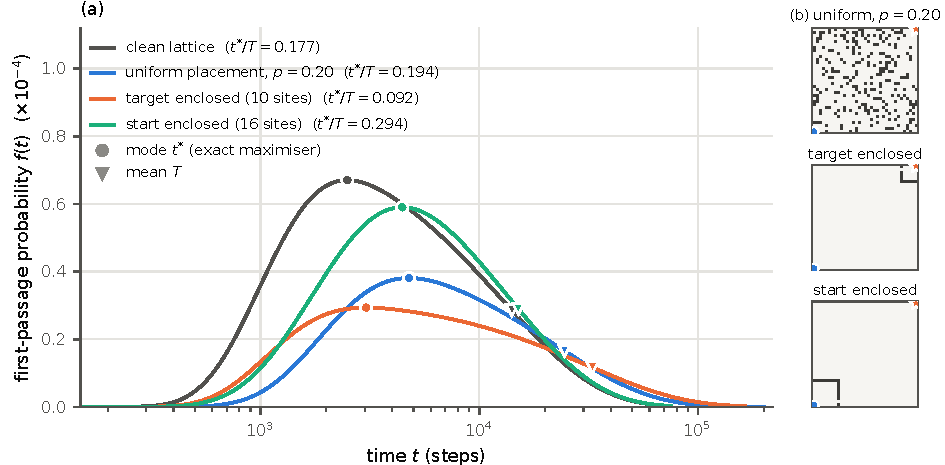
\includegraphics[width=\textwidth]{s7_defects_density_pmf.pdf}
% src: code/article/s7s8_defects_figures.py (fig_pmf); data data/msc_defects/structured_pmfs.npz, data/msc_defects/structured_masks.npz, data/msc_defects/structured_deterministic.csv, data/msc_defects/sweep/sweep_N35_uniform_p0.20.csv (rep 0)
\caption{Exact first-passage PMFs in discrete time for $N=35$, $q=0.8$, corner to opposite corner (logarithmic time
axis). (a)~Clean lattice, one uniform placement with $p=0.20$, and two deterministic geometries of
Section~\ref{s8_defects_placement:ssec-capture}: the target enclosed by $10$ blocked sites and the start enclosed by $16$, each
with a one-site opening. Circles mark the modes (exact maximisers), triangles the means; the legend gives
$\tmode/\MF$. (b)~The three configurations with blocked sites (dark; start: dot, bottom left; target: star, top
right).}
\label{s7_defects_density:fig-pmf}
\end{figure}

\subsection{The density sweep in full}\label{sup_defects:ssec-sweep}

\begin{table}[tbp]
\centering\small
\caption{Density sweep at $N=35$, $q=0.8$: samples~A and~B pooled ($800$ placements per row; $\pm$ is a $95\%$
interval over placements). ``acc.''\ is the fraction of drawn placements in which the target is connected to the
start. Time factors are ensemble means divided by the clean values $\MF=14\,100.8$ and $\tmode=2493$; $\Thetap(p)$ is
the homogenised factor \eqref{s7_defects_density:eq-theta}, estimate $\Thetap_{192}$ of
Table~\ref{s7_defects_density:tab-homog}. The
interval of $\langle\tmode\rangle/\langle\MF\rangle$ is a percentile bootstrap. Clean lattice: $\tmode/\MF=0.1768$,
CV $=0.918$.}
\label{s7_defects_density:tab-sweep}
\begin{tabular}{@{}lccccccc@{}}
\toprule
$p$ & acc. & $\langle\MF\rangle/\MF_{\mathrm{clean}}$ & $\langle\tmode\rangle/\tmode_{\mathrm{clean}}$ & $\Thetap(p)$ &
$\langle\tmode/\MF\rangle$ & $\langle\tmode\rangle/\langle\MF\rangle$ & CV \\
\midrule
\multicolumn{8}{@{}l}{\emph{uniform placement}}\\
0.02 & 1.00 & $1.046\pm0.006$ & $1.046\pm0.002$ & 1.045 & $0.1775\pm0.0006$ & $0.1768$ $[0.1761,\,0.1776]$ & 0.918 \\
0.04 & 1.00 & $1.106\pm0.010$ & $1.099\pm0.003$ & 1.096 & $0.1774\pm0.0009$ & $0.1756$ $[0.1744,\,0.1769]$ & 0.918 \\
0.06 & 0.99 & $1.163\pm0.012$ & $1.157\pm0.003$ & 1.152 & $0.1782\pm0.0011$ & $0.1758$ $[0.1744,\,0.1772]$ & 0.918 \\
0.08 & 0.98 & $1.221\pm0.015$ & $1.219\pm0.004$ & 1.216 & $0.1795\pm0.0012$ & $0.1765$ $[0.1750,\,0.1782]$ & 0.917 \\
0.10 & 0.98 & $1.290\pm0.017$ & $1.294\pm0.005$ & 1.289 & $0.1810\pm0.0014$ & $0.1773$ $[0.1756,\,0.1791]$ & 0.916 \\
0.12 & 0.96 & $1.396\pm0.022$ & $1.385\pm0.006$ & 1.372 & $0.1804\pm0.0016$ & $0.1754$ $[0.1733,\,0.1774]$ & 0.916 \\
0.14 & 0.94 & $1.488\pm0.024$ & $1.487\pm0.007$ & 1.469 & $0.1825\pm0.0018$ & $0.1766$ $[0.1744,\,0.1788]$ & 0.915 \\
0.16 & 0.89 & $1.569\pm0.026$ & $1.599\pm0.009$ & 1.583 & $0.1863\pm0.0019$ & $0.1802$ $[0.1779,\,0.1825]$ & 0.913 \\
0.18 & 0.89 & $1.688\pm0.030$ & $1.739\pm0.010$ & 1.719 & $0.1891\pm0.0021$ & $0.1821$ $[0.1796,\,0.1846]$ & 0.912 \\
0.20 & 0.85 & $1.825\pm0.033$ & $1.911\pm0.013$ & 1.877 & $0.1926\pm0.0022$ & $0.1851$ $[0.1825,\,0.1878]$ & 0.910 \\
0.25 & 0.70 & $2.303\pm0.046$ & $2.531\pm0.028$ & 2.489 & $0.2035\pm0.0029$ & $0.1943$ $[0.1911,\,0.1974]$ & 0.905 \\
0.30 & 0.50 & $3.075\pm0.065$ & $3.662\pm0.060$ & 3.739 & $0.2214\pm0.0039$ & $0.2105$ $[0.2063,\,0.2148]$ & 0.897 \\
0.35 & 0.24 & $4.205\pm0.093$ & $5.643\pm0.136$ & 7.564 & $0.2456\pm0.0046$ & $0.2373$ $[0.2324,\,0.2425]$ & 0.885 \\
\midrule
\multicolumn{8}{@{}l}{\emph{corner-thinned placement}}\\
0.02 & 1.00 & $1.027\pm0.003$ & $1.042\pm0.001$ & 1.045 & $0.1794\pm0.0003$ & $0.1792$ $[0.1788,\,0.1796]$ & 0.917 \\
0.04 & 1.00 & $1.060\pm0.005$ & $1.087\pm0.001$ & 1.096 & $0.1817\pm0.0006$ & $0.1812$ $[0.1805,\,0.1818]$ & 0.916 \\
0.06 & 1.00 & $1.092\pm0.006$ & $1.137\pm0.002$ & 1.152 & $0.1849\pm0.0007$ & $0.1841$ $[0.1834,\,0.1849]$ & 0.914 \\
0.08 & 1.00 & $1.133\pm0.008$ & $1.195\pm0.003$ & 1.216 & $0.1877\pm0.0009$ & $0.1865$ $[0.1853,\,0.1875]$ & 0.912 \\
0.10 & 1.00 & $1.182\pm0.010$ & $1.262\pm0.003$ & 1.289 & $0.1904\pm0.0010$ & $0.1887$ $[0.1875,\,0.1900]$ & 0.911 \\
0.12 & 1.00 & $1.237\pm0.012$ & $1.342\pm0.004$ & 1.372 & $0.1938\pm0.0011$ & $0.1918$ $[0.1903,\,0.1932]$ & 0.909 \\
0.14 & 0.99 & $1.300\pm0.014$ & $1.436\pm0.006$ & 1.469 & $0.1978\pm0.0013$ & $0.1952$ $[0.1936,\,0.1967]$ & 0.907 \\
0.16 & 0.99 & $1.390\pm0.017$ & $1.540\pm0.007$ & 1.583 & $0.1996\pm0.0016$ & $0.1959$ $[0.1940,\,0.1978]$ & 0.906 \\
0.18 & 0.99 & $1.458\pm0.020$ & $1.665\pm0.008$ & 1.719 & $0.2063\pm0.0017$ & $0.2019$ $[0.1997,\,0.2042]$ & 0.902 \\
0.20 & 0.98 & $1.606\pm0.023$ & $1.829\pm0.011$ & 1.877 & $0.2066\pm0.0020$ & $0.2014$ $[0.1990,\,0.2037]$ & 0.902 \\
0.25 & 0.94 & $2.040\pm0.043$ & $2.436\pm0.026$ & 2.489 & $0.2207\pm0.0029$ & $0.2111$ $[0.2073,\,0.2149]$ & 0.895 \\
0.30 & 0.81 & $2.833\pm0.066$ & $3.625\pm0.070$ & 3.739 & $0.2378\pm0.0041$ & $0.2262$ $[0.2215,\,0.2308]$ & 0.887 \\
0.35 & 0.49 & $4.008\pm0.102$ & $5.516\pm0.140$ & 7.564 & $0.2550\pm0.0050$ & $0.2433$ $[0.2381,\,0.2488]$ & 0.879 \\
\bottomrule
\end{tabular}
% src: data/article/s7_defects_density_pooled.csv and s7_defects_density_tables.txt (code/article/s7_defects_density_pooled.py), from data/msc_defects/sweep/*.csv (sample A) and data/msc_defects_verify/v03_sweep/*.csv (sample B); Theta: data/msc_defects/homogenization.json
\end{table}

Among the $20\,800$ configurations the largest single ratio is $0.48$ ($0.32$ for $p\le0.2$) and the smallest $0.062$. The
least-squares slope of the per-placement ratios against $p$ under uniform placement is $+0.081\pm0.009$ for $p\le0.2$ but
$+0.038\pm0.015$ for $p\le0.12$: the dependence is not linear (95\% intervals from heteroscedasticity-consistent standard
errors; $8001$ and $4801$ points). Under corner-thinned placement the slope is $+0.159\pm0.007$ for $p\le0.2$ ($8001$ points).
% src: data/article/s7_defects_density_pooled.json (ols_trend_ratio_vs_p: uniform_pmax0.20_P, uniform_pmax0.12_P, corner_thinned_pmax0.20_P; slope, slope_ci95_hc3, n)
Under corner-thinned placement the coefficient of variation
falls from $0.918$ to $0.902$ at $p=0.2$. In sample~A alone the mean of the per-placement ratios never falls below the clean
value $0.1768$, whereas under uniform placement the ratio of the ensemble means does ($0.1733$ to $0.1760$ at $p=0.04$,
$0.06$, $0.10$, $0.12$): at low density the sign of the small change depends on the estimator. For $p\ge0.30$ many drawn
placements are rejected (acceptance $0.496$ and $0.241$ under uniform placement in sample~A), so those rows describe an
ensemble conditioned on connectivity. The tables of each sample separately are in the repository.
% src: data/article/s7_defects_density_pooled.json (statements.max_ratio_any_placement, max_ratio_any_placement_p_le_0.20, min_ratio_any_placement; ols_trend_ratio_vs_p.uniform_pmax0.20_P, uniform_pmax0.12_P, corner_thinned_pmax0.20_P); data/article/s7_defects_density_pooled.csv (cv_P at p = 0.20); data/msc_defects/tables/sweep_uniform.md, sweep_smart.md; data/msc_defects/summary_sweep_N35.csv; data/article/appC_tables_checks.json (sweep_*)
Under corner-thinned placement the mode factor is $0.3$--$3.1\%$ below $\Thetap$ for $p\le0.2$ and the factor of the mean
$1.7$--$15\%$ below. At $p=0.35$, where one uniform placement in four connects the corners, neither the mean nor the mode
follows $\Thetap$ ($4.2$ and $5.6$ against $7.6$).
% src: data/article/s7_defects_density_pooled.json (statements.corner_thinned_mode_fac_over_theta_pct_by_p_pooled, corner_thinned_mfpt_fac_over_theta_pct_by_p_pooled); data/article/s7_defects_density_pooled.csv

\subsection{Effective medium}\label{sup_defects:ssec-emt}

Here $(\Lgr V)(\vx)=\sum_{\vy\sim\vx}[V(\vx)-V(\vy)]$ is the Laplacian of $\mathbb Z^{2}$ with unit conductances and $\pk$ the
potential kernel: $\Lgr\pk=-4\delta_{\mathbf 0}$, $\pk$ is invariant under the symmetries of the lattice, and
$\pk(\vx+\ve_1)-\pk(\vx-\ve_1)\to0$ as $|\vx|\to\infty$. Equivalently, the resistance between two sites at distance two
along an axis of the infinite lattice is $\pk(2\ve_1)/2=2-4/\pi$ \citep{Cserti2000}. In
Proposition~\ref{s7_defects_density:prop-dilute}, $U$ satisfies Kirchhoff's law at every remaining site and
$U(\vx)+Ex_1\to0$ as $|\vx|\to\infty$; at $\pm\ve_2$ the potential is $0$; and in (b) $U^{0}_{b}$ and $U_{b}$ are the
potential drops of $U^{0}(\vx)=-Ex_1$ and of $U$ (extended by any value at $\mathbf 0$) across bond $b$.

\emph{Proof of Proposition~\ref{s7_defects_density:prop-dilute}.}
(a) Put $U(\vx)=-Ex_1+\frac u4[\pk(\vx+\ve_1)-\pk(\vx-\ve_1)]$ on all of $\mathbb Z^{2}$, with a constant $u$. Then
$\Lgr U=u\,(\delta_{\ve_1}-\delta_{-\ve_1})$, because $x_1$ is harmonic, and $U(\vx)+Ex_1\to0$ at infinity. By the
symmetries of $\pk$, $U(\mathbf 0)=0$, $U(\pm\ve_2)=0$ and $U(-\ve_1)=-U(\ve_1)$, with
$U(\ve_1)=-E+\frac u4\,\pk(2\ve_1)=-E+u\,(1-2/\pi)$. Kirchhoff's law on the diluted lattice at a site $\vx\neq\mathbf 0$
reads $(\Lgr U)(\vx)-[U(\vx)-U(\mathbf 0)]\,\mathbf 1_{\vx\sim\mathbf 0}=0$. It holds at every site that is not a
neighbour of $\mathbf 0$, and at $\pm\ve_2$, where both terms vanish. At $\pm\ve_1$ it reads $u=U(\ve_1)$, that is,
$u=-E+u(1-2/\pi)$, so $u=-\pi E/2$. For uniqueness, the difference of two solutions is harmonic on the diluted
lattice, which is connected, and tends to zero at infinity; by the maximum principle on balls of
increasing radius, it vanishes.

(b) Since $U^{0}(\mathbf 0)=0$ and $\sum_{\vy\sim\mathbf 0}U^{0}(\vy)=0$, the sum is
$\sum_{\vy\sim\mathbf 0}[U^{0}(\mathbf 0)-U^{0}(\vy)][U(\mathbf 0)-U(\vy)]=\sum_{\vy\sim\mathbf 0}U^{0}(\vy)U(\vy)
=(-E)u+E(-u)=\pi E^{2}$, whatever value is given to $U(\mathbf 0)$. For the finite statement, let $U^{0}$ and $U$ satisfy
Kirchhoff's law at every non-boundary node before and after the removal of a set $R$ of bonds ($U$ is constant, with
an arbitrary value, on any part cut off from the boundary), and $\Pow^{0}=\sum_b(U^{0}_b)^{2}$,
$\Pow=\sum_{b\notin R}U_b^{2}$ the dissipated powers. For any function $V$ that vanishes on the boundary set, with drop $V_b$ across bond $b$,
Kirchhoff's law gives $\sum_bU^{0}_bV_b=0$ and $\sum_{b\notin R}U_bV_b=0$. With $V=U-U^{0}$ these read
$\sum_bU^{0}_bU_b=\Pow^{0}$ and $\sum_{b\notin R}U_bU^{0}_b=\Pow$; subtracting, $\Pow^{0}-\Pow=\sum_{b\in R}U^{0}_bU_b$.
\hfill$\square$

\emph{Derivation.} In a large sample of $n_{\mathrm s}$ sites under a mean field $E$ the clean lattice dissipates
$\Pow^{0}=n_{\mathrm s}E^{2}$ (one bond per site along the field, $\condz=1$) and the diluted one
$\Pow=(\cond/\condz)\,n_{\mathrm s}E^{2}$. If each of the $pn_{\mathrm s}$ blocked sites is treated as isolated in the
unperturbed field, Proposition~\ref{s7_defects_density:prop-dilute}(b) gives $\Pow^{0}-\Pow=pn_{\mathrm s}\pi E^{2}$,
the interaction between defects entering at order $p^{2}$. An open site is cut off only if its four neighbours are
blocked, so $\Pinf=1-p+\Order(p^{4})$, and \eqref{s7_defects_density:eq-theta} gives the rest. The step from one
defect to a density of defects is not proved here, hence the label. The law is not new. \citet{WatsonLeath1974}
measured the conductivity of a $137\times137$ conducting mesh from which sites were removed and gave an
effective-medium theory with $\cond/\condz=1-\pi p+\tfrac12\pi p^{2}$, whose linear term is the first relation of
\eqref{s7_defects_density:eq-dilute}. \citet{Nieuwenhuizen1986} calculated the diffusion coefficient and the
static conductivity of exactly this walk, a random walk on the square lattice with randomly excluded sites, as an
expansion in the fraction of excluded sites that is exact through the terms of order $p^{2}$; the coefficients are
printed in Eqs~(4.2) and~(4.3) of \citet{Ernst1987}; they are reproduced as \eqref{s7_defects_density:eq-second-order}
in the main text.
As a check that does not depend on the printed numbers we evaluated the pair term of this expansion ourselves
(minus one half of the sum, over all separations on a torus of $N_{\mathrm t}^{2}$ sites, of the loss of
conductivity caused by two removed sites minus twice that of one site; no random sampling): the coefficient of
$p^{2}$ in $\cond/\condz$ is $1.28614$ at $N_{\mathrm t}=256$ and $1.28588$ after extrapolation in
$N_{\mathrm t}^{-2}$, which gives $-0.85571$ for the diffusivity; both are within $10^{-4}$ of the printed values.
% src: data/article/s7_defects_density_second_order.json (a2_largest_torus, a2_extrapolated_linear_in_Nt^-2_last3, D2_coefficient_from_extrapolated_a2, Nt2_times_(a2_minus_extrapolated)_last4, extrapolated_minus_published, check_two_sites_against_dense_solve, check_l1_against_stored_single_site); code/article/s7_defects_density_second_order.py
Numerical conductivities of diluted networks go back to \citet{Kirkpatrick1973}.
% src: Watson and Leath (1974), abstract (formula, lattice size and experimental nature quoted from it); Nieuwenhuizen, van Velthoven and Ernst (1986), abstract ("exact to O(c^2) terms included"); Ernst, Nieuwenhuizen and van Velthoven (1987), full text read: Eqs (4.2), (4.3) and Table 2, row b = 1 (their conductivity and diffusion coefficient carry the prefactor 1/4 of the unit-rate walk, omitted here)

Three numerical checks support \eqref{s7_defects_density:eq-dilute}. One blocked site on a torus of
$N_{\mathrm t}\times N_{\mathrm t}$ sites gives
$(1-\cond/\condz)N_{\mathrm t}^{2}=3.064378$, $3.122318$, $3.136774$, $3.140388$, $3.141291$, $3.141517$ for
$N_{\mathrm t}=8,16,\dots,256$ ($\pi=3.141593$), identically in both codes. % src: data/msc_defects/homogenization.json (single_site); data/msc_defects_verify/v04_homog.json (single)
In a square of $(2j+1)^{2}$ sites with the potential fixed on two opposite sides, the potential next to a
removed central site and the loss of power are $0.99602$, $0.99901$, $0.99975$, $0.99994$, $0.99998$ times $-\pi E/2$
and $\pi E^{2}$ for $j=10,20,40,80,160$. % src: data/article/s7_defects_density_dipole_check.json (finite)
At finite $p$, $\cond$ and $\Pinf$ were measured on tori three times
(Table~\ref{s7_defects_density:tab-homog}); we write $\Thetap_{192}$, $\Thetap_{160}$ and $\Thetap_{200}$ for the
three estimates of $\Thetap$, after the side of the torus. $\Thetap_{192}$ (12 placements per density) is
$1.045$, $1.289$, $1.877$ and $3.739$ at $p=0.02$, $0.1$, $0.2$ and $0.3$; $\Thetap_{160}$ (10 placements,
second code) agrees with it within its intervals; and $\Thetap_{200}$ (40 placements, second code, computed for
$p=0.1$ and $0.2$ only) is the most precise: $1.2877\pm0.0012$ and $1.8783\pm0.0057$.
% src: data/msc_defects/homogenization.json (finite_p); data/msc_defects_verify/v04_homog.json (random, L160); data/msc_defects_verify/v04b_theta.json; data/article/derived_checks.json (H_three_estimates_of_Theta)
Beyond first order the measurements can be compared with \eqref{s7_defects_density:eq-second-order}, which has no
free parameter. The measured conductivity is $\cond/\condz=0.9378$, $0.6981$ and $0.4253$ at $p=0.02$, $0.10$ and
$0.20$, against $0.9377$, $0.6987$ and $0.4231$ from the exact expansion truncated after $p^{2}$ and $0.9378$,
$0.7015$ and $0.4345$ from the effective-medium expression of \citet{WatsonLeath1974}. Measurement and truncated
expansion differ by at most $6.2\times10^{-4}$ at the eleven densities with $p\le0.18$, which is inside the $95\%$ interval
of the measurement at ten of them, and by $+0.0022$ ($\pm0.0015$) at $p=0.20$. The measured coefficient of $p^{2}$,
$(\cond/\condz-1+\pi p)/p^{2}$, averaged over $p=0.06$--$0.14$ with inverse-variance weights, is $1.26\pm0.03$,
against the exact $1.2858$ and the effective-medium value $\pi/2=1.571$. For the diffusivity, $\Deff/\Dzero$ lies
below the linear law by $0.0017$, $0.0101$ and $0.0389$ at $p=0.04$, $0.10$ and $0.20$, of which the term
$-0.8558\,p^{2}$ supplies $0.0014$, $0.0086$ and $0.0342$. The remainder corresponds to a third-order coefficient
of about $-0.9$ ($-0.95\pm0.48$ at $p=0.14$, $-0.87\pm0.28$ at $p=0.18$). That is the value, $-0.8558$, which the
factor $1/\Pinf=1/(1-p)$ in \eqref{s7_defects_density:eq-theta} generates from \eqref{s7_defects_density:eq-second-order}
when the conductivity has no third-order term; the measured third-order coefficient of the conductivity is indeed
compatible with zero ($-0.05\pm0.42$ and $+0.04\pm0.23$ at the same two densities). The third-order statements are
measurements, not derived coefficients.
% src: data/article/derived_checks.json (E_dilute_laws: rows[*].sigma, sigma_ci95, sigma_exact_to_second_order_ENvV1987, sigma_minus_exact_second_order, sigma_Watson_Leath_EMT, D_minus_linear, D_implied_third_order_coeff(+_ci95), sigma_implied_third_order_coeff(+_ci95); max_abs_sigma_minus_exact_second_order_p_le_0.18; n_densities_p_le_0.18_with_sigma_within_ci95_of_exact_second_order; sigma_second_order_coeff_weighted_mean_p0.06_to_0.14); data/article/s7_defects_density_pooled.json (homogenisation.finite_p.D_minus_dilute); coefficients 1.2858 and -0.8558: Ernst, Nieuwenhuizen and van Velthoven (1987), Eqs (4.2), (4.3)

\begin{table}[tbp]
\centering\small
\caption{Homogenised transport coefficients of the site-diluted square lattice with uniformly placed blocked sites.
Columns~2--6: $192\times192$ tori, $12$ placements per $p$ ($\pm$: $95\%$ interval; $\Pinf$ is the fraction of sites
in the largest cluster); column~6 is the estimate $\Thetap_{192}$. $\Thetap_{160}$: independent estimate from
$160\times160$ tori, $10$ placements. $\Thetap_{200}$: $200\times200$ tori, $40$ placements.}
\label{s7_defects_density:tab-homog}
\setlength{\tabcolsep}{4pt}
\begin{tabular}{@{}lccccccc@{}}
\toprule
$p$ & $\cond/\condz$ & $\Pinf$ & $\Deff/\Dzero$ & $1-(\pi-1)p$ & $\Thetap_{192}$ & $\Thetap_{160}$ & $\Thetap_{200}$ \\
\midrule
0.02 & $0.9378\pm0.0002$ & 0.9800 & 0.9569 & 0.9572 & 1.045 & $1.0450\pm0.0003$ & -- \\
0.04 & $0.8761\pm0.0003$ & 0.9600 & 0.9126 & 0.9143 & 1.096 & $1.0956\pm0.0008$ & -- \\
0.06 & $0.8160\pm0.0004$ & 0.9400 & 0.8681 & 0.8715 & 1.152 & $1.1517\pm0.0018$ & -- \\
0.08 & $0.7568\pm0.0006$ & 0.9200 & 0.8227 & 0.8287 & 1.216 & $1.2138\pm0.0017$ & -- \\
0.10 & $0.6981\pm0.0009$ & 0.8999 & 0.7757 & 0.7858 & 1.289 & $1.2883\pm0.0033$ & $1.2877\pm0.0012$ \\
0.14 & $0.5852\pm0.0011$ & 0.8596 & 0.6808 & 0.7002 & 1.469 & $1.4685\pm0.0042$ & -- \\
0.20 & $0.4253\pm0.0015$ & 0.7983 & 0.5328 & 0.5717 & 1.877 & $1.883\pm0.013$ & $1.8783\pm0.0057$ \\
0.25 & $0.2994\pm0.0022$ & 0.7453 & 0.4017 & 0.4646 & 2.489 & $2.490\pm0.042$ & -- \\
0.30 & $0.1840\pm0.0024$ & 0.6878 & 0.2675 & 0.3575 & 3.739 & $3.79\pm0.09$ & -- \\
0.35 & $0.0815\pm0.0023$ & 0.6166 & 0.1322 & 0.2504 & 7.564 & $7.25\pm0.63$ & -- \\
\bottomrule
\end{tabular}
% src: data/msc_defects/homogenization.json (finite_p), data/msc_defects/tables/homogenization.md; data/msc_defects_verify/v04_homog.json (random, L160); data/msc_defects_verify/v04b_theta.json (L200); rows generated by code/article/s7_defects_density_pooled.py -> data/article/s7_defects_density_tables.txt (the Theta_200 column added from v04b_theta.json)
\end{table}


\subsection{Size dependence and the whole distribution}\label{sup_defects:ssec-size}

\emph{Larger lattices.} For uniform placement at $p=0.1$ and $0.2$ we computed certified modes up to $N=200$ and
means up to $N=280$ (Table~\ref{s7_defects_density:tab-size}, Fig.~\ref{s7_defects_density:fig-size}), using
the most precise estimate, $\Thetap_{200}(0.1)=1.2877$ and $\Thetap_{200}(0.2)=1.8783$.
\begin{itemize}
\item The mode factor equals $\Thetap$ to within $1.11\%$ at $p=0.1$ and $1.6\%$ at $p=0.2$ for every $N$ from $15$ to
$200$, and within its interval for $N\ge70$.
\item The factor of the mean divided by $\Thetap$, averaged over $N=35$--$280$ with inverse-variance weights, is
$1.004\pm0.005$ at $p=0.1$ and $0.987\pm0.007$ at $p=0.2$.
\item The shift of $\langle\tmode/\MF\rangle$ relative to the clean lattice of the same size is between $+0.6\%$ and
$+1.2\%$ for $N\ge50$ at $p=0.1$, with intervals of $\pm1.0$ to $\pm1.8\%$. At $p=0.2$ it falls from $+9.4\pm1.8\%$ at
$N=35$ to $+4.5\pm1.4\%$ at $N=100$, $+2.9\pm1.8\%$ at $N=140$ and $+3.9\pm2.7\%$ at $N=200$: it halves but is not
shown to vanish. About half of it is the Jensen gap; the ratio of ensemble means is shifted by $+5.3\%$, $+2.2\%$,
$+0.5\%$ and $+2.4\%$ at $N=35$, $100$, $140$ and $200$.
\end{itemize}
% src: data/article/s7_defects_density_pooled.json (size_dependence.summary); data/msc_defects_verify/v07_summary.csv, v07b_summary.csv, v04b_theta.json
In the smaller sample~A ($40$--$100$ placements per size for $N\ge70$; open symbols in
Fig.~\ref{s7_defects_density:fig-size}(b)) both time factors agree with $\Thetap$ within their intervals at these
sizes; the larger sample~B is needed to quantify the residual shift of the ratio at $p=0.2$.
% src: data/msc_defects/summary_size.csv (N >= 70: mfpt_factor, mode_factor with intervals; ratio_shift +0.0051 at N = 140 with ratio_ci 0.0057)

\emph{Whole distribution.} Mean and mode are two functionals of the distribution. Comparing each placement's
survival function, in units of its own $\MF$, with the clean one in units of its $\MF$ ($N=35$, $200$ uniform
placements per $p$, $0\le t\le6\,\MF$), the Kolmogorov distance averages $0.008$ at $p=0.1$ and $0.013$ at $p=0.2$
(largest values $0.027$ and $0.039$). The same distance is $0.023$ to $0.072$ for five of the deterministic obstacle
geometries of Section~\ref{s8_defects_placement:ssec-det} and $0.008$ for the most favourable phase of the period-3
array (the phase tabulated in Table~\ref{appC_tables:tab-deterministic}).
% src: data/msc_defects_verify/v11_shape.json (periodic_a3, single phase); data/article/derived_checks.json (D_periodic_phases["3"]: tabulated_is_smallest_mean_factor)

In summary, for uniformly random blocked sites time dilation by $\Thetap(p)$ is accurate at $p=0.1$ and is a
$1$--$3\%$ approximation at $p=0.2$ at the sizes computed, where $\langle\tmode/\MF\rangle$ is still $3$--$4.5\%$ above
its clean value at $N=100$--$200$. A slow approach is to be expected: in \eqref{s7_defects_density:eq-resistance} the constant that
accompanies the logarithm of $N$ in $\Glap_{\va\va}$ is set by the immediate surroundings of the target and need not
scale with $\condz/\cond$. The limit itself is not established.

\begin{table}[tbp]
\centering\small
\caption{Size dependence under uniform placement ($q=0.8$; $\pm$ is a $95\%$ interval over placements;
$\Thetap$ is the estimate $\Thetap_{200}$ of Table~\ref{s7_defects_density:tab-homog}). $K$:
placements with certified modes; ``shift'' is the relative difference between the ratio with defects and the clean
ratio at the same $N$, for the mean of per-placement ratios and for the ratio of ensemble means (percentile-bootstrap
interval). $K'$: placements of a separate sample for which only the mean was computed. Both samples are from the
second code.}
\label{s7_defects_density:tab-size}
\begin{tabular}{@{}lcccccc@{}}
\toprule
$N$ & $K$ & $\langle\tmode\rangle/\tmode_{\mathrm{clean}}$ & shift of $\langle\tmode/\MF\rangle$ (\%) &
shift of $\langle\tmode\rangle/\langle\MF\rangle$ (\%) & $K'$ & $\langle\MF\rangle/(\Thetap\,\MF_{\mathrm{clean}})$ \\
\midrule
\multicolumn{7}{@{}l}{$p=0.1$, $\Thetap=1.2877\pm0.0012$}\\
15 & 200 & $1.283\pm0.015$ & $+4.8\pm2.0$ & $+2.3$ $[+0.1,\,+4.7]$ & -- & -- \\
25 & 200 & $1.302\pm0.011$ & $+2.0\pm1.8$ & $-0.6$ $[-2.8,\,+1.7]$ & -- & -- \\
35 & 400 & $1.294\pm0.007$ & $+2.9\pm1.1$ & $+1.1$ $[-0.3,\,+2.3]$ & 800 & $1.007\pm0.014$ \\
50 & 200 & $1.296\pm0.009$ & $+1.2\pm1.6$ & $-0.7$ $[-2.4,\,+1.1]$ & 800 & $1.008\pm0.012$ \\
70 & 400 & $1.293\pm0.006$ & $+0.9\pm1.0$ & $-0.8$ $[-2.1,\,+0.4]$ & 800 & $1.009\pm0.012$ \\
100 & 300 & $1.290\pm0.005$ & $+1.1\pm1.0$ & $-0.1$ $[-1.2,\,+1.0]$ & 600 & $0.990\pm0.010$ \\
140 & 200 & $1.288\pm0.006$ & $+1.1\pm1.1$ & $+0.1$ $[-1.2,\,+1.3]$ & 400 & $1.008\pm0.014$ \\
200 & 60 & $1.290\pm0.009$ & $+0.6\pm1.8$ & $-0.1$ $[-2.0,\,+1.6]$ & 300 & $1.017\pm0.018$ \\
280 & -- & -- & -- & -- & 200 & $1.006\pm0.018$ \\
\midrule
\multicolumn{7}{@{}l}{$p=0.2$, $\Thetap=1.8783\pm0.0057$}\\
15 & 200 & $1.908\pm0.054$ & $+9.8\pm3.7$ & $+3.7$ $[-0.4,\,+8.1]$ & -- & -- \\
25 & 200 & $1.900\pm0.033$ & $+8.3\pm2.9$ & $+3.1$ $[-0.2,\,+6.5]$ & -- & -- \\
35 & 400 & $1.905\pm0.019$ & $+9.4\pm1.8$ & $+5.3$ $[+3.2,\,+7.3]$ & 800 & $0.986\pm0.018$ \\
50 & 200 & $1.899\pm0.021$ & $+8.1\pm2.3$ & $+4.3$ $[+1.6,\,+7.2]$ & 800 & $0.977\pm0.016$ \\
70 & 400 & $1.888\pm0.013$ & $+5.4\pm1.5$ & $+1.9$ $[+0.2,\,+3.8]$ & 800 & $0.988\pm0.015$ \\
100 & 300 & $1.886\pm0.012$ & $+4.5\pm1.4$ & $+2.2$ $[+0.6,\,+3.7]$ & 600 & $0.989\pm0.016$ \\
140 & 200 & $1.890\pm0.014$ & $+2.9\pm1.8$ & $+0.5$ $[-1.3,\,+2.6]$ & 400 & $0.980\pm0.017$ \\
200 & 60 & $1.868\pm0.019$ & $+3.9\pm2.7$ & $+2.4$ $[-0.6,\,+5.2]$ & 300 & $1.001\pm0.021$ \\
280 & -- & -- & -- & -- & 200 & $0.994\pm0.022$ \\
\bottomrule
\end{tabular}
% src: data/msc_defects_verify/v07_summary.csv (modes), v07b_summary.csv (means), v04b_theta.json (Theta); rows generated by code/article/s7_defects_density_pooled.py -> data/article/s7_defects_density_tables.txt
\end{table}

\begin{figure}[tbp]
\centering
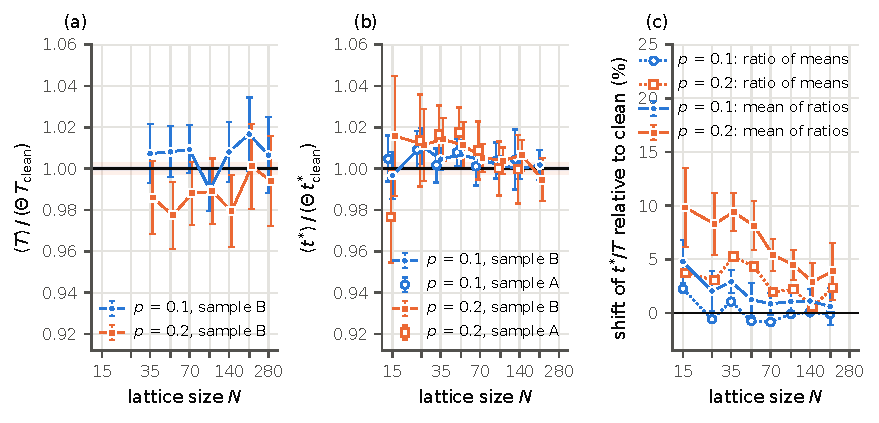
\includegraphics[width=\textwidth]{s7_defects_density_size.pdf}
% src: code/article/s7_defects_density_figures.py (adapted from code/msc_defects_verify/v10_figures.py, vfig3); data data/msc_defects_verify/v07_summary.csv, v07b_summary.csv, v04b_theta.json; data/msc_defects/summary_size.csv
\caption{Size dependence of time dilation under uniform placement, $q=0.8$, corner to opposite corner, discrete time;
circles $p=0.1$, squares $p=0.2$ (displaced horizontally for clarity); bars are $95\%$ intervals over placements, and
the shaded bands the $95\%$ intervals of $\Thetap_{200}$. (a)~Ensemble mean of $\MF$ divided by $\Thetap\,\MF_{\mathrm{clean}}$
($200$--$800$ placements per point, sample~B). (b)~Ensemble mean of $\tmode$ divided by $\Thetap\,\tmode_{\mathrm{clean}}$:
filled symbols sample~B ($60$--$400$ placements), open symbols sample~A ($40$--$200$ placements). (c)~Shift of
$\tmode/\MF$ relative to the clean lattice of the same $N$ (sample~B): mean of per-placement ratios (filled, solid) and
ratio of ensemble means (open, dotted).}
\label{s7_defects_density:fig-size}
\end{figure}

\subsection{What controls the mean and the mode}\label{sup_defects:ssec-mechanism}

Placements with one of the two neighbours of the target blocked have a mean larger by 20--31\% and a mode
larger by 6--9\% than those of the same ensemble with both open (two placement laws, $p=0.1$ and $0.2$,
sample~A; 21--33\% and 8--10\% in sample~B).
% src: data/msc_defects/summary_stratified.csv; data/msc_defects_verify/v09_mechanism.json; data/article/s8_defects_placement_checks.json (stratified_sample_A, stratified_sample_B)
Two other explanations are not supported. The shortest open path between the corners keeps its clean length of
68 steps in every placement up to $p=0.1$ and has mean length $68.06$ at $p=0.2$ ($68.04$ in sample~B): the
direct route is not lengthened.
% src: data/msc_defects/summary_sweep_N35.csv (chem_dist, uniform); data/msc_defects_verify/v09_mechanism.json (relax_p0.10, relax_p0.20)
Nor do dead ends set the modal time: the relaxation time of the reflecting cluster, whose slowest mode localises
on weakly attached pockets, grows by a factor $2.21$ at $p=0.2$ and $6.6$ at $p=0.3$ ($2.18\pm0.04$ and
$6.3\pm0.5$ in sample~B), while the mode grows by $1.92$ and $3.70$ (sample~A), close to $\Thetap=1.88$ and
$3.74$.
% src: data/msc_defects/summary_sweep_N35.csv (tau_rel_factor, mode_factor, hom_factor; uniform); data/msc_defects_verify/v09_mechanism.json (relax_p0.20, relax_p0.30)

\begin{figure}[tbp]
\centering
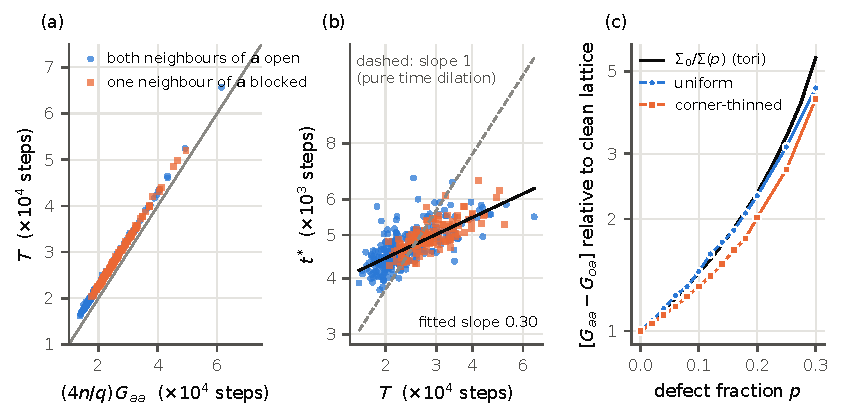
\includegraphics[width=\textwidth]{s8_defects_placement_mechanism.pdf}
\caption{What controls the mean and the mode ($N=35$, $q=0.8$, corner to opposite corner, discrete time).
(a)~Exact mean first-passage time against $(4\nn/q)\Glap_{\va\va}$ for the 400 uniform placements of sample~A at
$p=0.2$; the line is the diagonal, and the offset from it is the cross term $-(4\nn/q)\Glap_{\vo\va}$.
(b)~Mode against mean for the same placements, logarithmic axes; solid line: least-squares fit (slope $0.30$);
dashed line: slope 1, the behaviour under a pure dilation of time.
(c)~Ensemble mean of $\Glap_{\va\va}-\Glap_{\vo\va}$ relative to the clean lattice for the uniform and the
corner-thinned placement (400 placements per point), and the homogenised value
$\condz/\cond(p)$ of Section~\ref{s7_defects_density:ssec-emt}.}
% src: data/msc_defects/sweep/sweep_N35_uniform_p0.20.csv, data/msc_defects/summary_sweep_N35.csv, data/msc_defects/homogenization.json; drawn by code/article/s8_defects_placement_figures.py
\label{s8_defects_placement:fig-mechanism}
\end{figure}

\subsection{Single-defect susceptibilities}\label{sup_defects:ssec-susc}

Let $\chi_A(\vx)=A_{\vx}/A_{\mathrm{clean}}-1$ be the relative change of $A\in\{\MF,\tmode\}$ when the single
site $\vx\ne\vo,\va$ is blocked (Fig.~\ref{s8_defects_placement:fig-maps}). Because one defect shifts the mode
by a few steps at most, the position of the maximum is refined to a fraction of a step by a parabola through
$\pmf(\tmode-1)$, $\pmf(\tmode)$, $\pmf(\tmode+1)$.

\begin{figure}[tbp]
\centering
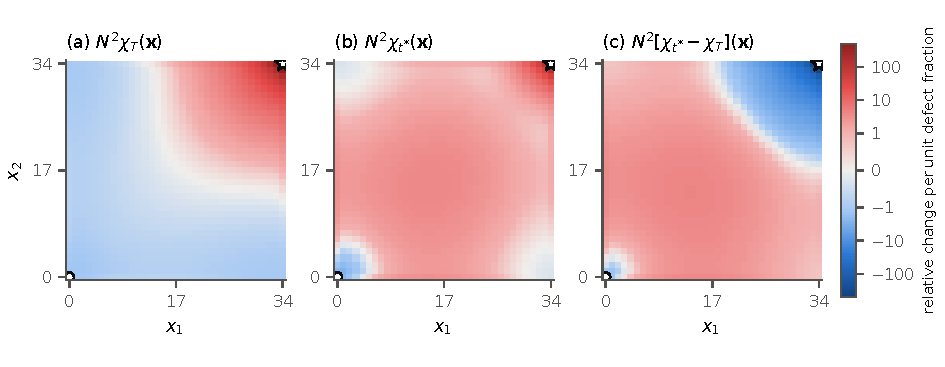
\includegraphics[width=\textwidth]{s8_defects_placement_maps.pdf}
\caption{Single-defect susceptibilities at $N=35$, $q=0.8$ (discrete time): each site is blocked alone and the
exact mean and mode are recomputed. (a)~$N^{2}\chiT(\vx)$, (b)~$N^{2}\chim(\vx)$, (c)~their difference.
Circle: start; star: target.
The colour scale is linear between $-1$ and $1$ and logarithmic beyond. Blue sites shorten the first-passage
statistic when blocked.}
% src: data/msc_defects/sensitivity_N35.csv (figure: code/article/s7s8_defects_figures.py, fig_maps)
\label{s8_defects_placement:fig-maps}
\end{figure}

\emph{Blocking a single site shortens the mean first-passage time for $67.6\%$ of the sites} ($60.1\%$ at $N=15$,
$65.3\%$ at $N=25$).
% src: data/msc_defects/summary_first_order.json; data/msc_defects_verify/v05_sens_N15.json, v05_sens_N25.json, v05_sens_N35.json
Far from the target the only effect is the lost volume, $\chiT\approx-1/\nn=-8.2\times10^{-4}$ (minimum
$-1.04\times10^{-3}$); the positive values are concentrated around the target, with a maximum of $+38.2\%$ for
either of its neighbours. Of $\sum_{\vx}\chiT(\vx)$, $64\%$, $88\%$ and $105\%$ come from sites within Euclidean
distance 3, 6 and 10 of the target. The mode behaves differently: only $5.4\%$ of the sites lower it, its
largest response is $+10.5\%$ (the same two sites), and the corresponding shares of $\sum_{\vx}\chim(\vx)$ are
$19\%$, $25\%$ and $28\%$: its response is spread over the whole region between start and target.
% src: data/msc_defects/summary_first_order.json; data/msc_defects_verify/v05_sens_N35.json; data/article/s8_defects_placement_checks.json (susceptibility_N35)

For a placement law with site probabilities $w(\vx)$, $\sum_{\vx}w(\vx)=1$, adding the effects of the $pN^{2}$
single defects gives the first-order estimate
\begin{equation}\label{s8_defects_placement:eq-first-order}
  \frac{\dif\ln\langle A\rangle}{\dif p}\bigg|_{p=0}=N^{2}\sum_{\vx}w(\vx)\,\chi_A(\vx).
\end{equation}
This is first-order perturbation theory, not a theorem; Table~\ref{s8_defects_placement:tab-slopes} compares it
with measured secants. For uniform placement the two slopes nearly coincide, so the ratio hardly moves at first
order ($\dif\ln(\tmode/\MF)/\dif p=-0.09$), and both approach the bulk value $\pi-1=2.142$ of
\eqref{s7_defects_density:eq-dilute} from above: $(2.291,2.227)$, $(2.278,2.197)$ and $(2.271,2.183)$ for
$N=15$, $25$ and $35$.
% src: data/msc_defects/summary_first_order.json; data/msc_defects_verify/v05_sens_N15.json, v05_sens_N25.json, v05_sens_N35.json

\begin{table}[tbp]
\centering
\caption{First-order slopes \eqref{s8_defects_placement:eq-first-order} at $N=35$ and measured secants
$(\langle A\rangle/A_{\mathrm{clean}}-1)/p$ at $p=25/1225$ (400 placements per sample, $\pm$ 95\% confidence
interval). The secants contain the second-order terms, which the estimate omits.}
\label{s8_defects_placement:tab-slopes}
\begin{tabular}{llccc}
\toprule
placement & statistic & first order & secant, sample A & secant, sample B\\
\midrule
uniform        & mean & $2.271$ & $2.12\pm0.41$ & $2.37\pm0.42$\\
uniform        & mode & $2.183$ & $2.21\pm0.12$ & $2.30\pm0.12$\\
corner-thinned & mean & $1.261$ & $1.30\pm0.17$ & $1.39\pm0.23$\\
corner-thinned & mode & $1.923$ & $2.04\pm0.05$ & $2.04\pm0.07$\\
\bottomrule
\end{tabular}
% src: data/msc_defects/summary_first_order.json (first order; sample A); data/msc_defects_verify/v03_summary.csv via data/article/s8_defects_placement_checks.json (secants_p002, sample B); data/msc_defects_verify/v05_sens_N35.json (first order, separately written code)
\end{table}

The same estimate explains why the ratio rises under corner-thinned placement
(Section~\ref{s7_defects_density:ssec-sweep}). That law thins the defects inside the $4\times4$ boxes at the start
and target corners, to $55\%$ of the uniform probability on average. The box at the target holds $71\%$ of
$\sum\chiT$ but only $21\%$ of $\sum\chim$ (the box at the start less than $1\%$ of either, in absolute value).
Thinning lowers the slope of the mean from $2.27$ to $1.26$ and that of the mode only from $2.18$ to $1.92$, so
the ratio must rise: $\dif\ln(\tmode/\MF)/\dif p=+0.66$, that is $\dif(\tmode/\MF)/\dif p=0.177\times0.66=+0.12$ at
$p=0$.
% src: data/msc_defects_verify/v05_sens_N35.json (share_*_in_target_box, share_*_in_start_box, cornerthinned_weight_ratio_in_target_box); data/msc_defects/summary_first_order.json (pred_slope_ratio); data/article/s8_defects_placement_checks.json (susceptibility_N35)
The rise is a consequence of where the placement law puts the defects, not of their density.

\subsection{Localised placements, deterministic geometries and periodic arrays}\label{s8_defects_placement:ssec-det}

Forty blocked sites are $3.3\%$ of the lattice. Near the target they multiply the mean by $3.37\pm0.13$
($3.43\pm0.13$ in sample~B) and the mode by $1.36$, and the ratio falls to $0.0752\pm0.0022$
($0.0741\pm0.0021$), less than half its clean value. Near the start they leave the mean unchanged
($\times0.999\pm0.003$; $\times1.002\pm0.004$), delay the mode by a third, and raise the ratio to
$0.2329\pm0.0040$ ($0.2368\pm0.0048$). In the centre the ratio is $0.2015$; anywhere on the lattice, $0.1771$.
With ten blocked sites near the start the mean is \emph{below} its clean value in all 200 placements of either
sample.
% src: data/msc_defects/summary_structured_local.csv (mfpt_factor, mode_factor, ratio, frac_mfpt_below_clean); data/msc_defects_verify/v06_local.csv via data/article/s8_defects_placement_checks.json (local_sample_B); data/msc_defects_verify/v06.log
Hence $\tmode/\MF$ is not a function of the defect density. It decreases when the defects surround the target,
increases when they lie around the start or between start and target, and, when they are spread uniformly, stays within
a few per cent of its clean value at low density ($p\le0.14$) but rises by $4.7\%$ to $8.9\%$, depending on the
estimator, at $p=0.2$ (Section~\ref{sup_defects:ssec-sweep}).
% src: data/article/s7_defects_density_pooled.json (statements.uniform_ratio_excess_pct_by_p, uniform_rom_excess_pct_by_p: p = 0.14 and 0.20)

Table~\ref{s8_defects_placement:tab-det} lists a selection of the 28 deterministic geometries of
Table~\ref{appC_tables:tab-deterministic} and Fig.~\ref{s8_defects_placement:fig-structured}(a); all were computed
twice with separately written programs (identical modes, means equal to $2\times10^{-11}$).
% src: data/msc_defects/structured_deterministic.csv; data/msc_defects_verify/v06_det.csv; data/article/appC_tables_checks.json (deterministic_second_implementation_max_rel_diff_mfpt)

\begin{table}[tbp]
\centering
\caption{Selected deterministic geometries ($N=35$, $q=0.8$; exact values). A wall is a full column of blocked
sites with a gap; a serpentine consists of equally spaced walls with three-site gaps on alternating sides; an
enclosure is an L-shaped wall at Chebyshev distance $R$ from a corner with a one-site door, the second site from
the lattice edge. CV is the coefficient of variation of the first-passage time.}
\label{s8_defects_placement:tab-det}
\begin{tabular}{lrcccc}
\toprule
geometry & blocked & $\MF$ factor & $\tmode$ factor & $\tmode/\MF$ & CV\\
\midrule
clean lattice                                   &   0 & $1$     & $1$     & $0.1768$ & $0.918$\\
mid-lattice wall, one-site gap                  &  34 & $1.760$ & $3.139$ & $0.3153$ & $0.855$\\
serpentine, three walls                         &  96 & $3.537$ & $6.773$ & $0.3385$ & $0.820$\\
wall near the target, three-site gap            &  32 & $2.284$ & $1.741$ & $0.1348$ & $0.949$\\
enclosure of the target, $R=5$                  &  10 & $2.332$ & $1.219$ & $0.0925$ & $0.963$\\
enclosure of the start, $R=5$                   &  10 & $1.018$ & $1.248$ & $0.2168$ & $0.895$\\
solid $12\times12$ block at the centre          & 144 & $0.954$ & $1.233$ & $0.2284$ & $0.890$\\
solid $6\times6$ block near the start           &  36 & $0.971$ & $1.002$ & $0.1825$ & $0.913$\\
\bottomrule
\end{tabular}
% src: data/msc_defects/structured_deterministic.csv; data/msc_defects_verify/v06_det.csv
\end{table}

Walls and corridors push the law towards the one-dimensional shape: the five serpentines have
$\tmode/\MF=0.316$--$0.339$ and a coefficient of variation of $0.820$--$0.847$, against $1/3$ and $0.816$ for the
clean chain (Section~\ref{s5_modes:sec}); such obstacles lengthen the transit more than the capture.
% src: data/msc_defects/structured_deterministic.csv via data/article/s8_defects_placement_checks.json (deterministic)
Enclosing the target does the opposite and makes the law more nearly exponential (ratio $0.0925$, coefficient of
variation $0.963$ for ten blocked sites), while the same ten sites around the start change the mean by $1.8\%$.
A solid $12\times12$ block in the centre \emph{lowers} the mean by $4.6\%$ ($13\,459$ against $14\,101$ steps) and
delays the mode by $23\%$: it removes $11.8\%$ of the volume and adds only $8.2\%$ to
$\Glap_{\va\va}-\Glap_{\vo\va}$.
% src: data/msc_defects/structured_deterministic.csv; data/msc_defects_verify/v06_det.csv; data/article/s8_defects_placement_checks.json (deterministic.block12_centre)

For a periodic array with one blocked site per $A\times A$ cell the response at $N=35$ depends on the phase of
the array relative to the target. For $A=3$ the mean factor ranges from $1.08$ to $1.47$ over the nine phases
(average $1.23$) and the mode factor from $1.18$ to $1.32$ (average $1.24$); the phases that block a neighbour of
the target give $1.47$, more than the average $1.30$ of uniformly random placements at $p=0.1$. The periodic
rows of Table~\ref{appC_tables:tab-deterministic} are single phases: for $A=3$ and $A=2$ the phase with the
smallest mean factor ($1.08$ and $1.25$; ranges $1.08$--$1.47$ and $1.25$--$1.54$), for $A=4$ the twelfth
smallest of the sixteen ($1.16$; range $1.03$--$1.43$, average $1.14$).
% src: data/msc_defects_verify/v06_periodic.csv via data/article/s8_defects_placement_checks.json (periodic_phases) and data/article/derived_checks.json (D_periodic_phases); data/msc_defects/summary_sweep_N35.csv (uniform, p = 0.10, mfpt_factor)
In the bulk the comparison is cleaner. The unit-cell problem of the infinite array, solved in rational
arithmetic, gives $\cond/\condz=1/2$, $5/7$ and $14/17$ for $A=2$, $3$ and $4$, so that by
\eqref{s7_defects_density:eq-theta} the time factors are $3/2$, $56/45=1.244$ and $255/224=1.138$, against about
$2.49$, $1.33$ and $1.16$ for random placement at the same densities $1/4$, $1/9$ and $1/16$ (interpolated from
the values behind Table~\ref{s7_defects_density:tab-homog}).
% src: data/article/s8_defects_placement_checks.json (periodic_bulk); data/msc_defects/homogenization.json
A periodic array is thus a much weaker obstruction than a random one at $p=1/4$, but only $7\%$ weaker at
$p=1/9$ and $2\%$ at $p=1/16$.

\subsection{A two-time-scale heuristic}\label{sup_defects:ssec-twotime}

Why does an obstacle near the target move the mean so much more than the mode? The following argument is a
heuristic: it accounts for the sign and the approximate size of the effect and has no controlled error.

Beyond the transit time the first-passage probability is dominated by the two slowest terms $j=0,1$ of the
spectral sum \eqref{s2_model:eq-spectral}. In the time constants $\Tcap=-1/\ln(1-q\nu_0)$ of the slowest term (the
capture time) and $\tau_1=-1/\ln(1-q\nu_1)$ of the next,
\begin{equation}\label{s8_defects_placement:eq-two-time-form}
  \pmf(t)\approx q\,b_0\,\eu^{-t/\Tcap}\bigl[1-c\,\eu^{-t/\tau}\bigr],\qquad c=-\frac{b_1}{b_0}>0,\qquad
  \frac1\tau=\frac1{\tau_1}-\frac1{\Tcap},
\end{equation}
where a shift of $t$ by one step is neglected. Its maximiser is the discrete-time form of the two-exponential
maximiser $\ln(-b_1\nu_1/b_0\nu_0)/(\nu_1-\nu_0)$ of Section~\ref{s6_mechanism:ssec-two-pole}, since
$1/\tau$ corresponds to $q(\nu_1-\nu_0)$ and $c\,(1+\Tcap/\tau)$ to $-b_1\nu_1/(b_0\nu_0)$:
\begin{equation}\label{s8_defects_placement:eq-two-time}
  \tmode\approx\tau\,\ln\Bigl[c\Bigl(1+\frac{\Tcap}{\tau}\Bigr)\Bigr],\qquad
  \frac{\partial\ln\tmode}{\partial\ln\Tcap}\bigg|_{\tau,c}=\frac{\tau}{\tmode}\;\frac{\Tcap/\tau}{1+\Tcap/\tau}.
\end{equation}
What is new here is only the question asked of it: how the maximiser moves when an obstacle changes $\Tcap$.
On the clean lattice $\Tcap=12\,935$ steps, $\tau_1=518.0$ steps, hence $\tau=540$, and $c=4.15$; the two-term sum
peaks at $t=2506$ and three terms give the exact mode $2493$ (Fig.~\ref{s8_defects_placement:fig-two-time}(a)).
% src: data/msc_defects_verify/v09_mechanism.json (two_mode); data/article/s8_defects_placement_checks.json (two_time); data/article/s7s8_defects_figures.json (two_time)
The rate $\nu_1$ is the one that \eqref{s6_mechanism:eq-poles} places at $\muone(1+W/X)$, a time constant of 528
steps. It must not be confused with the relaxation time of the reflecting lattice, 621 steps: of the two
degenerate slowest modes, the combination that is odd under exchange of the coordinates vanishes on the diagonal
and has zero weight in the corner-to-corner law ($10^{-31}$ against $8.5\times10^{-5}$ numerically).
% src: data/msc_defects_verify/v09_mechanism.json (clean_top_modes_lam_w_tau); data/article/s8_defects_placement_checks.json (two_time.closed_form_sec6.second_time_constant, slowest_reflecting_time)

A pure dilation multiplies $\Tcap$ and $\tau$ by the same factor and leaves $\tmode/\MF$ unchanged. A perturbation
that raises only the capture time moves the mode sub-linearly, with the exponent of
\eqref{s8_defects_placement:eq-two-time}, $0.21$ on the clean lattice when $\tau$ and $c$ are held fixed. If instead
$\tau_1$ and $c$ are held fixed, $\tau$ follows $\Tcap$ ($\dif\tau/\dif\Tcap=-\tau^{2}/\Tcap^{2}$) and the exponent is
$0.17$.
% src: data/article/s8_defects_placement_checks.json (two_time.elasticity_formula, two_time.elasticity_formula_tau1_c_fixed)
The exact elasticities $\ln(\tmode\ \text{factor})/\ln(\MF\ \text{factor})$ of obstacles that enclose the target
or block one of its neighbours are
somewhat larger: $0.310$ for one blocked neighbour of the target, $0.255$, $0.234$ and $0.269$ for enclosures
with $R=3$, $5$ and $8$, $0.241$ for $R=5$ with a three-site door
(Fig.~\ref{s8_defects_placement:fig-two-time}(b)), and $0.247$--$0.253$ for the near-target ensembles of
Table~\ref{s8_defects_placement:tab-local} in both samples.
% src: data/msc_defects_verify/v09b_twotime.csv (elasticity_exact); data/article/s8_defects_placement_checks.json (near_target_elasticity)
With $\tau$ and $c$ frozen and $\Tcap$ multiplied by its exact factor, \eqref{s8_defects_placement:eq-two-time}
gives mode factors of $1.072$, $1.170$, $1.188$, $1.202$ and $1.102$ for these five deterministic cases, against
the exact $1.105$, $1.215$, $1.219$, $1.279$ and $1.116$, that is 69--88\% of the logarithmic shift; the rest
arises because $\tau_1$ and $c$ change as well ($\tau_1$ rises from 518 to 543 steps for one blocked neighbour).
The closed-form approximation \eqref{s6_mechanism:eq-L1}, evaluated with the clean-lattice $\muone$, $A$, $W$ and
the exact mean of the perturbed lattice, lets $\nu_1$ move with the mean and errs on the other side: $1.107$,
$1.247$, $1.272$, $1.294$ and $1.150$.
% src: data/msc_defects_verify/v09b_twotime.csv (pred_tau540, mode_fac_exact, tau_sub2); data/article/s8_defects_placement_checks.json (two_time.cases)
The heuristic fails for the sixth deterministic case examined, the wall near the target of
Table~\ref{s8_defects_placement:tab-det} (mean $\times2.284$, mode $\times1.741$): that obstacle also lengthens the
transit, $\tau_1$ rises from 518 to 1163 steps, the exact elasticity is $0.67$, and the frozen-$\tau$ formula
($1.180$) accounts for only $30\%$ of the logarithmic shift of the mode.
% src: data/msc_defects_verify/v09b_twotime.csv (row wall_neartarget_gap_centre_g3: elasticity_exact, pred_tau540, tau_sub1); data/article/s8_defects_placement_checks.json (two_time.cases[5])

In short, a change of the capture time alone moves the mode with an exponent of about $1/4$ at $N=35$, so that
$\tmode/\MF$ falls roughly as $\MF^{-3/4}$ when defects surround the target without obstructing the transit
($0.1768\times3.37^{-3/4}=0.071$
against the measured $0.075$ for forty sites); an obstacle that also changes $\tau_1$, such as a wall, is outside
this estimate. The fluctuations at fixed density show the same behaviour: across
the 400 uniform placements at $p=0.2$ the regression of $\ln\tmode$ on $\ln\MF$ has slope $0.30$ (sample~A;
$0.31$ in sample~B; Fig.~\ref{s8_defects_placement:fig-mechanism}(b)). The exponent is not universal: by
\eqref{s8_defects_placement:eq-two-time} it is close to $1/\ln[c(1+\Tcap/\tau)]$, which decreases slowly as $N$
grows.
% src: data/article/s8_defects_placement_checks.json (power_law_check_M40_near_target, two_time.cross_placement_slope_p02); data/msc_defects_verify/v09_mechanism.json (p0.20.loglog_slope_mode_on_mfpt)

\begin{figure}[tbp]
\centering
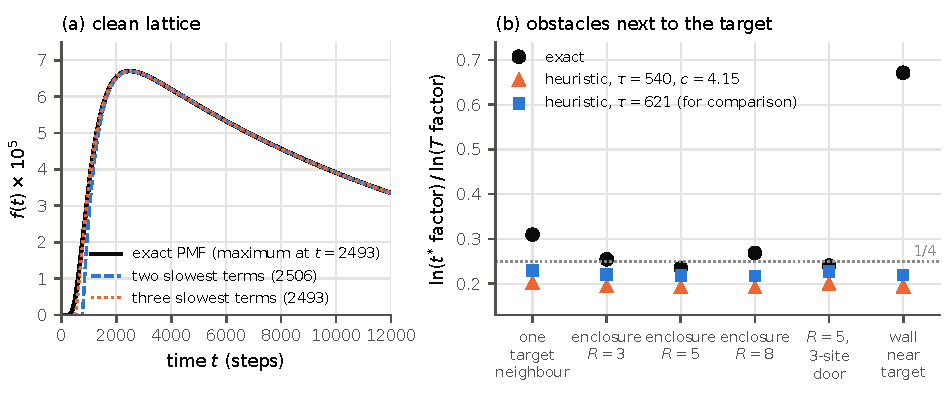
\includegraphics[width=\textwidth]{s8_defects_placement_twotime.pdf}
\caption{Two time scales ($N=35$, $q=0.8$, corner to opposite corner, discrete time). (a)~Exact first-passage
probability of the clean lattice and its truncations to the two and three slowest terms with non-zero weight
(the legend gives the position of each maximum; the truncations are drawn only where they are on scale).
(b)~Elasticity of the mode with respect to the mean for the six deterministic obstacles examined: exact values
(circles) and the heuristic \eqref{s8_defects_placement:eq-two-time} with $\tau$ and $c$ frozen, either at the
values taken from the spectrum ($\tau=540$, $c=4.15$; triangles) or with $\tau$ set to the relaxation time 621 of the
reflecting lattice and $c$ fitted to the clean mode (squares). The second choice is shown for comparison only:
that mode has zero weight in the corner-to-corner law. The heuristic fails for the wall near the target, which
also lengthens the transit.}
% src: data/msc_defects_verify/v09b_twotime.csv (all six rows); spectrum of the clean lattice recomputed by code/article/s7s8_defects_figures.py (fig_twotime) -> data/article/s7s8_defects_figures.json
\label{s8_defects_placement:fig-two-time}
\end{figure}

\subsection{A one-parameter family of shapes}

Over all 13\,631 exactly solved configurations of sample~A (10\,402 random placements of the density sweep, 3200
localised placements, the clean lattice and the 28 deterministic geometries) the coefficient of variation is nearly a function of
$\ratio=\tmode/\MF$ alone (Fig.~\ref{s8_defects_placement:fig-shape}): the Pearson correlation is $-0.981$, and
the quadratic $\mathrm{CV}=1.0073-0.4564\,\ratio-0.2461\,\ratio^{2}$ fits with a root-mean-square residual of
$0.0045$. The 67 configurations ($0.5\%$) with a residual above $0.02$, the largest being $0.235$, are all
random placements with $p\ge0.25$, towards the percolation threshold; over the whole sample $\ratio$ ranges from
$0.047$ to $0.469$ and the coefficient of variation from $0.729$ to $1.125$.
% src: data/article/s8_defects_placement_checks.json (shape_family.sample_A); data/msc_defects_verify/v09_mechanism.json (family_main_implementation); data/article/derived_checks.json (G_shape_family_extent)
The 13\,629 configurations of sample~B give a correlation of $-0.983$ and, with their own quadratic, a residual of
$0.0041$ (largest $0.14$).
% src: data/msc_defects_verify/v09_mechanism.json (family_recheck)
Clean lattices with $N=10$--$200$ lie on the same curve (residuals between $-0.0033$ and $+0.0004$); the clean
one-dimensional chain, $(1/3,\,0.8165)$, lies $0.011$ below it, at the end of the trend rather than on the curve.
% src: data/article/s8_defects_placement_checks.json (shape_family.sample_A.clean_resid, chain_1d_resid); data/msc_defects_verify/v09_mechanism.json (family_clean_resid_main_implementation_quadratic, family_1d_point_resid)
We record this as an empirical regularity of the model, without a theory: size, defect density and defect
placement appear to act mainly by moving the law along one line between a transit-limited shape and a
capture-limited, nearly exponential one.

\begin{figure}[tbp]
\centering
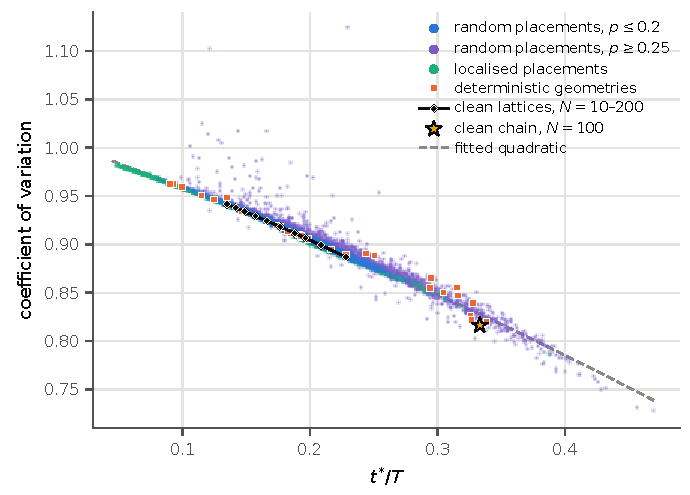
\includegraphics{s8_defects_placement_shape.pdf}
\caption{Coefficient of variation against $\tmode/\MF$ for all 13\,631 exactly solved configurations of sample~A
($N=35$, $q=0.8$, corner to opposite corner, discrete time; every configuration lies inside the frame): random
placements of the density sweep (both placement laws; $p\le0.2$ and $p\ge0.25$ in different colours), localised
placements, deterministic geometries, the clean lattices with
$N=10$--$200$, and the clean one-dimensional chain with $N=100$. Dashed: the quadratic of the text.}
% src: data/msc_defects/sweep/*.csv, structured_local.csv, structured_deterministic.csv, size_clean.csv, beyond_1d_random.csv; data/article/s8_defects_placement_checks.json (shape_family.sample_A.quad_c0_c1_c2); figure: code/article/s7s8_defects_figures.py (fig_shape) -> data/article/s7s8_defects_figures.json (n_configurations_plotted, frame)
\label{s8_defects_placement:fig-shape}
\end{figure}

\subsection{Other defect types}\label{sup_defects:ssec-other}

\paragraph{One dimension: permeable bonds.} A blocked site between start and target disconnects them, so the
inert model is empty in one dimension. Its analogue is a bond that is crossed with a reduced probability.

\begin{proposition}[Chain with barriers]\label{s8_defects_placement:prop-1d-barriers}
On $\{0,\dots,N-1\}$ let the walker cross the bond between $k$ and $k+1$ with probability $w_k>0$ per step in
either direction ($k=0,\dots,N-2$) and stay otherwise, with a reflecting end at $0$ and
$w_{k-1}+w_{k}\le1$ for $1\le k\le N-2$. Then
\begin{equation}\label{s8_defects_placement:eq-1d-barriers}
  \MF_{0\to N-1}=\sum_{k=0}^{N-2}\frac{k+1}{w_k}.
\end{equation}
\end{proposition}
\begin{proof}
The transition matrix is symmetric and irreducible, so all mean hitting times are finite
(Proposition~\ref{s2_model:prop-pinv}). Let $h_k$ be the mean time to reach $k+1$ from $k$. From site $0$ the
walker moves to $1$ with probability $w_0$ per step and stays otherwise, so $h_0=1/w_0$. For $k\ge1$ condition on
the first step: with probability $w_k$ the walker arrives; with probability $w_{k-1}$ it moves to $k-1$, needs
$h_{k-1}$ steps on average to return to $k$ and then, by the strong Markov property, $h_k$ more; otherwise it
stays at $k$. Hence $h_k=1+w_{k-1}(h_{k-1}+h_k)+(1-w_{k-1}-w_k)h_k$, that is $w_kh_k=1+w_{k-1}h_{k-1}$, and by
induction $w_kh_k=k+1$. A nearest-neighbour walk started at $0$ reaches $N-1$ by passing from $k$ to $k+1$ for
$k=0,\dots,N-2$ in turn, so $\MF_{0\to N-1}=\sum_kh_k$.
\end{proof}

This is a case of the classical formula for passage times of birth-and-death chains
\citep[see, e.g.,][]{LevinPeresWilmer2009}. For a single barrier it is Eq.~(12) of \citet{SarvaharmanGiuggioli2023}:
a barrier between start and target raises the mean linearly in its distance from the reflecting end, whereas a barrier
behind the start leaves the mean unchanged while it changes the mode and the tail, the `disorder indifference' of
these authors (with the start at the reflecting end, as here, every barrier lies between start and target). With $w_k=q/2$ it returns $\MF=N(N-1)/q$ \eqref{s4_mfpt:eq-1d}; with
barriers, $w_k=\perm_kq/2$ and $\MF=(2/q)\sum_k(k+1)/\perm_k$. In the terms of
Section~\ref{s8_defects_placement:ssec-capture}, $1/w_k$ is the resistance of bond $k$ and $k+1$ the number of
sites upstream of it: a barrier costs more the nearer it is to the target. For independent, identically
distributed $\perm_k$ the disorder average is $\langle\MF\rangle=\MF_{\mathrm{clean}}\langle1/\perm\rangle$ exactly, for
every $N$. For $N=100$ and $q=0.8$ (clean values $\MF=12\,375$, $\tmode=4124$, ratio $0.3333$) one barrier with
$\perm=0.1$ moves $\tmode/\MF$ between $0.313$ (bond 77) and $0.353$ (bond 21); when each bond is a barrier
with $\perm=0.2$ with probability $p$, the ensemble mean of the ratio stays between $0.3317$ and $0.3336$ for
$p=0.05$--$0.5$ in both samples (400 chains per $p$, confidence intervals $\pm0.0010$ to $\pm0.0015$)
(Fig.~\ref{s8_defects_placement:fig-beyond}(a)).
% src: data/msc_defects/summary_beyond.json (1d_random, 1d_single); data/msc_defects_verify/v08_beyond.json (1d_clean, 1d_single_k0.1, 1d_random); data/article/s8_defects_placement_checks.json (chain_barriers)
Uniformly random barriers in one dimension are again a dilation of time.

\paragraph{Two dimensions: permeable obstacles.} Let every bond that touches a defect site be crossed with
probability $\perm q/4$ per step ($\perm=0$: inert site; $\perm=1$: clean lattice), refused attempts being
cancelled as before; an analytic framework for lattice walks with inert heterogeneities is given by
\citet{SarvaharmanGiuggioli2023}.
At $p=0.1$ (100 uniform placements per sample) and $\perm=0.01$, $0.1$, $0.3$, $0.6$ the ratio is
$0.1797\pm0.0041$, $0.1788\pm0.0031$, $0.1786\pm0.0019$, $0.1778\pm0.0009$ in sample~A and $0.1824\pm0.0038$,
$0.1811\pm0.0028$, $0.1800\pm0.0017$, $0.1785\pm0.0008$ in sample~B: within $1.6\%$ and $3.2\%$ of the clean
value, an excess of the size found for inert sites at this density, while mean and mode move together
(Fig.~\ref{s8_defects_placement:fig-beyond}(b)).
% src: data/msc_defects/summary_beyond.json (2d_permeable); data/msc_defects_verify/v08_beyond.json (perm); data/article/s8_defects_placement_checks.json (permeable)
The limit $\perm\to0^{+}$ is singular. A site that can be entered at all carries its full share of the uniform
stationary distribution, so that $\nn$ in \eqref{s7_defects_density:eq-resistance} jumps from $(1-p)N^{2}$ to
$N^{2}$: at $\perm=10^{-3}$ the mean is $20\,656\pm797$, against $18\,616/0.9=20\,685$ from the inert mean
(sample~B: $20\,113\pm825$ against $18\,121/0.9=20\,135$). The mode, reached long before the slow sites
equilibrate, stays near its inert value ($3292\pm46$ against $3245\pm40$), and the ratio drops to
$0.1628\pm0.0037$ ($0.1648\pm0.0034$ in sample~B).
% src: data/msc_defects/summary_beyond.json (2d_permeable, kappa = 0, 0.001); data/msc_defects_verify/v08_beyond.json (perm); data/article/s8_defects_placement_checks.json (permeable)

\paragraph{Partial traps.} A partial trap removes a walker standing on a defect site with probability $\trap$ per step
($\trap\le1-q$); it is obtained by subtracting $\trap$ from the diagonal element of the transition matrix at every defect
site. The first-passage law is then defective. At $p=0.1$
(100 placements per sample) and $\trap=10^{-5}$, $10^{-4}$, $10^{-3}$, $10^{-2}$ the probability
$P_{\mathrm{hit}}$ of ever reaching the target is $0.9861$, $0.8758$, $0.3912$, $0.0277$ (sample~B: $0.9861$, $0.8756$, $0.3907$, $0.0277$); killing
at the uniform rate $p\trap$ on the clean lattice, for which this probability is $\Ftil(1-p\trap)$, gives
$0.9861$, $0.8752$, $0.3887$, $0.0256$. The mean conditional on arrival falls ($13\,936$, $12\,621$, $6797$,
$1896$ steps), the mode moves less ($2486$, $2429$, $2060$, $1210$), and their ratio rises: $0.178$, $0.192$,
$0.303$, $0.638$ ($0.178$, $0.192$, $0.303$, $0.639$ in sample~B; Fig.~\ref{s8_defects_placement:fig-beyond}(c)).
% src: data/msc_defects/summary_beyond.json (2d_traps); data/msc_defects_verify/v08_beyond.json (traps)
Traps remove the long trajectories and act in the opposite sense to obstacles.

\begin{figure}[tbp]
\centering
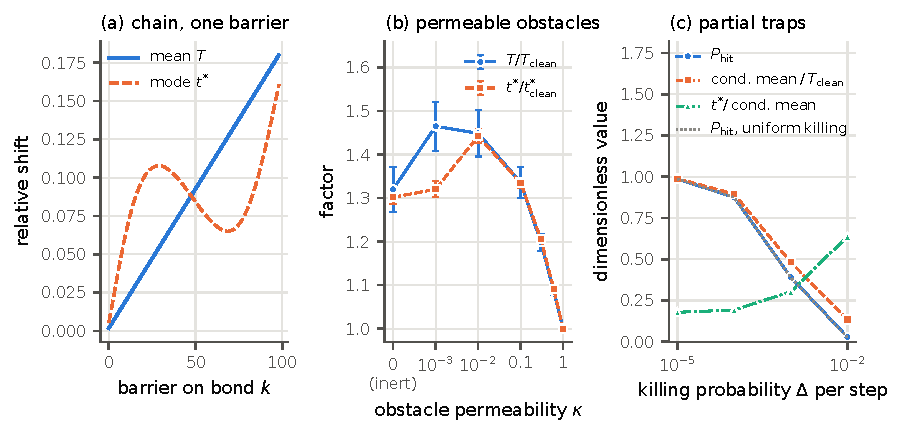
\includegraphics[width=\textwidth]{s8_defects_placement_beyond.pdf}
\caption{Other defect types (discrete time, $q=0.8$; sample~A). (a)~Chain with $N=100$ and one barrier of
permeability $\perm=0.1$ on bond $k$: relative shift of the mean, from \eqref{s8_defects_placement:eq-1d-barriers},
and of the mode. (b)~$N=35$, corner to opposite corner, permeable obstacles on $10\%$ of the sites: mean and mode
relative to the clean lattice against $\perm$ (100 placements; bars: 95\% confidence intervals). (c)~The same
placements with partial traps of killing probability $\trap$: probability $P_{\mathrm{hit}}$ of reaching the
target, the same under uniform killing at rate $p\trap$ (dotted), conditional mean relative to the clean mean, and
mode divided by the conditional mean.}
% src: data/msc_defects/beyond_1d_single.csv, summary_beyond.json; drawn by code/article/s8_defects_placement_figures.py
\label{s8_defects_placement:fig-beyond}
\end{figure}


% sections/appC_tables.tex -- Supplementary Section S10: extended tables.
% Body only.  Labels: prefix "appC_tables:".
% The numerical rows of all tables are generated from the result files by  code/article/appC_tables_build.py
% (fragments in data/article/appC_tables_fragments/, cross-checks and derived numbers in
% data/article/appC_tables_checks.json).  Do not edit those rows by hand:
% `python code/article/appC_tables_build.py --check'  verifies that they are verbatim copies.
% Paths in "% src:" comments are relative to the root of the repository (see README.md).
%
% local helpers (no new notation): ragged-right cell, and a group that sets the tables in a smaller
% size while the captions stay in the normal size
\providecommand{\appCrr}{\raggedright\hspace{0pt}}
\providecommand{\appCtablesetup}{%
  \footnotesize
  \setlength{\LTcapwidth}{\textwidth}%
  \setlength{\tabcolsep}{4pt}%
  \renewcommand{\tablename}{\normalsize Table}}

\section{Extended tables}\label{appC_tables:sec}

This section gives the full tables behind Sections~\ref{s3_methods:sec}--\ref{s7_defects:sec} of the main text. The
numerical rows are copied from the result files by a script, not retyped; only the typography differs from the sources.
% src: code/article/appC_tables_build.py; data/article/appC_tables_checks.json
Unless stated otherwise, times are in steps, $q=0.8$, and the walk goes from one corner to the opposite corner (\CC).

\subsection{Exact modes and means}\label{appC_tables:ssec-modes}

All rows of Tables~\ref{appC_tables:tab-T1}--\ref{appC_tables:tab-T3} up to $N=10\,240$ are certified global maximisers
(Proposition~\ref{s3_methods:prop-certificate}; for $N=10\,240$ see Section~\ref{sup_methods:ssec-certificate}). The last
two rows of Table~\ref{appC_tables:tab-T1} are the local maxima of \eqref{s5_modes:eq-1d-pmf} nearest the continuum
prediction, located in double precision and confirmed in 50-digit arithmetic; they are the global maximisers by
Theorem~\ref{s6b_rigorous:thm-1d}(c) (computer-assisted). The ratios of the three large-$N$ rows, $0.33328426$,
$0.33328427$ and $0.33328427$, agree with the limit~\eqref{s5_modes:eq-1d-ratio} to seven decimals.
% src: data/msc_modes_verify/bigN_1d_mp.json; data/msc_modes/laplace_modes.jsonl (d = 1: mode_discrete_q0.8); data/article/appC_tables_checks.json (T1_large_N_rows); data/article/s3_methods_certificate.json (CC_q0.8_d1, CC_q0.8_d2, CC_q0.8_d3); data/article/s3_methods_certificate_chain.json (certified_global_maximiser, N = 10240)

\begingroup\appCtablesetup
% src: data/msc_modes/tables.md (Table T1, 15 of 33 rows, exact columns); last three rows: data/msc_modes_verify/bigN_1d_mp.json and data/article/appC_tables_checks.json (T1_large_N_rows)
\begin{longtable}{@{}rrrr@{}}
\caption{One dimension, reflecting end to absorbing end, $q=0.8$, discrete time: exact mode $\tmode$ and mean
$\MF=N(N-1)/q$ (15 of the 33 computed sizes, and three larger sizes).}
\label{appC_tables:tab-T1}\\
\toprule
$N$ & $\tmode$ & $\MF$ & $\tmode/\MF$ \\
\midrule
\endfirsthead
\multicolumn{4}{@{}l}{\emph{Table~\thetable\ (continued)}} \\
\toprule
$N$ & $\tmode$ & $\MF$ & $\tmode/\MF$ \\
\midrule
\endhead
\bottomrule
\endfoot
$5$ & $8$ & $25$ & $0.32000$ \\
$9$ & $29$ & $90$ & $0.32222$ \\
$13$ & $64$ & $195$ & $0.32821$ \\
$17$ & $113$ & $340$ & $0.33235$ \\
$21$ & $174$ & $525$ & $0.33143$ \\
$25$ & $249$ & $750$ & $0.33200$ \\
$29$ & $338$ & $1015$ & $0.33300$ \\
$35$ & $495$ & $1487.5$ & $0.33277$ \\
$50$ & $1020$ & $3062.5$ & $0.33306$ \\
$70$ & $2012$ & $6037.5$ & $0.33325$ \\
$100$ & $4124$ & $12\,375$ & $0.33325$ \\
$140$ & $8107$ & $24\,325$ & $0.33328$ \\
$200$ & $16\,580$ & $49\,750$ & $0.33327$ \\
$400$ & $66\,490$ & $199\,500$ & $0.33328$ \\
$1000$ & $416\,188$ & $1.24875\times10^{6}$ & $0.33328$ \\
\midrule
$10\,240$ & $43\,679\,969$ & $131\,059\,200$ & $0.33328$ \\
$100\,000$ & $4\,166\,011\,658$ & $12\,499\,875\,000$ & $0.33328$ \\
$1\,000\,000$ & $416\,604\,915\,263$ & $1\,249\,998\,750\,000$ & $0.33328$ \\
\end{longtable}
\endgroup

\begingroup\appCtablesetup
% src: data/msc_modes/tables.md (Table T2, 15 of 31 rows, exact columns)
\begin{longtable}{@{}rrrr@{}}
\caption{Two dimensions, \CC, $q=0.8$, discrete time: exact mode and mean (15 of the 31 computed sizes). Means are
printed to six significant figures.}
\label{appC_tables:tab-T2}\\
\toprule
$N$ & $\tmode$ & $\MF$ & $\tmode/\MF$ \\
\midrule
\endfirsthead
\multicolumn{4}{@{}l}{\emph{Table~\thetable\ (continued)}} \\
\toprule
$N$ & $\tmode$ & $\MF$ & $\tmode/\MF$ \\
\midrule
\endhead
\bottomrule
\endfoot
$5$ & $36$ & $133.523$ & $0.2696$ \\
$9$ & $136$ & $582.819$ & $0.2333$ \\
$13$ & $304$ & $1413.12$ & $0.2151$ \\
$17$ & $541$ & $2662.84$ & $0.2032$ \\
$21$ & $849$ & $4359.64$ & $0.1947$ \\
$25$ & $1228$ & $6525.22$ & $0.1882$ \\
$29$ & $1679$ & $9177.43$ & $0.1829$ \\
$35$ & $2493$ & $14\,100.8$ & $0.1768$ \\
$50$ & $5253$ & $31\,614.8$ & $0.1662$ \\
$70$ & $10\,570$ & $67\,212.4$ & $0.1573$ \\
$100$ & $22\,110$ & $148\,521$ & $0.1489$ \\
$140$ & $44\,248$ & $312\,092$ & $0.1418$ \\
$200$ & $92\,116$ & $682\,335$ & $0.1350$ \\
$301$ & $212\,975$ & $1.6634\times10^{6}$ & $0.1280$ \\
$401$ & $383\,013$ & $3.09907\times10^{6}$ & $0.1236$ \\
\end{longtable}
\endgroup

\begingroup\appCtablesetup
% src: data/msc_modes/tables.md (Table T3, all 17 rows, exact columns)
\begin{longtable}{@{}rrrr@{}}
\caption{Three dimensions, \CC, $q=0.8$, discrete time: exact mode and mean (all computed sizes). Means are printed to
six significant figures.}
\label{appC_tables:tab-T3}\\
\toprule
$N$ & $\tmode$ & $\MF$ & $\tmode/\MF$ \\
\midrule
\endfirsthead
\multicolumn{4}{@{}l}{\emph{Table~\thetable\ (continued)}} \\
\toprule
$N$ & $\tmode$ & $\MF$ & $\tmode/\MF$ \\
\midrule
\endhead
\bottomrule
\endfoot
$5$ & $85$ & $555.333$ & $0.1531$ \\
$7$ & $187$ & $1616.08$ & $0.1157$ \\
$9$ & $332$ & $3545.23$ & $0.0936$ \\
$11$ & $523$ & $6602.02$ & $0.0792$ \\
$13$ & $760$ & $11\,045.7$ & $0.0688$ \\
$15$ & $1044$ & $17\,135.5$ & $0.0609$ \\
$17$ & $1376$ & $25\,130.6$ & $0.0548$ \\
$19$ & $1757$ & $35\,290.2$ & $0.0498$ \\
$25$ & $3202$ & $81\,348.9$ & $0.0394$ \\
$30$ & $4759$ & $141\,444$ & $0.0336$ \\
$35$ & $6644$ & $225\,599$ & $0.0295$ \\
$40$ & $8863$ & $337\,864$ & $0.0262$ \\
$50$ & $14\,323$ & $662\,926$ & $0.0216$ \\
$60$ & $21\,175$ & $1.14903\times10^{6}$ & $0.0184$ \\
$70$ & $29\,447$ & $1.82859\times10^{6}$ & $0.0161$ \\
$80$ & $39\,161$ & $2.734\times10^{6}$ & $0.0143$ \\
$100$ & $62\,998$ & $5.35199\times10^{6}$ & $0.0118$ \\
\end{longtable}
\endgroup

\subsection{Scaling fits}\label{appC_tables:ssec-fits}

Each law is fitted by least squares to $\ln\tmode$ on $10\le N\le200$ ($10\le N\le100$ for $\dd=3$). The data are exact,
so half-widths and residuals measure misfit, not noise. Inside the window the laws are hard to tell apart; outside it
they are not: a pure $N^{2}$ law for $\dd=2$ is $30.80\%$ too low at $N=16\,777\,216$, and a pure $N^{3}$ law for $\dd=3$ is
$6798.98\%$ too high at $N=4096$. On the information criterion $A N^{a}(\ln N)^{b}$ is preferred to $N^{2}(A\ln\ln N+B)$ in
both two-dimensional panels, so the fits do not reveal the $\ln\ln N$ law, which is proved, with a slowly decaying
remainder, in Theorem~\ref{s6b_rigorous:thm-laws}.
% src: data/msc_modes/tables.md (fit tables); data/msc_modes/fit_results.json (fits)
A second implementation reproduces parameters and extrapolation errors to the printed digits; its $\Delta\mathrm{AICc}$
values differ by at most $2.8$ units, without changing a ranking.
% src: data/msc_modes_verify/analysis.json (fits); data/msc_modes/fit_results.json (fits); data/checks/modes_scaling_fits_recheck.json (max_abs_dAICc_difference = 2.786, ranking_by_AICc_identical_in_every_window, params_max_rel_diff = 1.0e-7)

\begingroup\appCtablesetup\setlength{\tabcolsep}{3pt}
% src: data/msc_modes/tables.md (tables "2D mode (continuous time, unit rate): fit on N = 10..200, extrapolated", "3D mode (continuous time, unit rate): fit on N = 10..100, extrapolated", "2D mode, exact discrete PMF, q = 0.8, N = 11..200", "3D mode, exact discrete PMF, q = 0.8, N = 11..100"); data/msc_modes/fit_results.json (fits: n_points, holdout_N)
\begin{longtable}{@{}lp{3.7cm}rrrrrrr@{}}
\caption{Least-squares fits of $\ln\tmode$ against $N$ (\CC). Parameters are given with the half-width of their
95\% least-squares interval in brackets; ``rms'' and ``max'' are the root-mean-square and the largest absolute
residual of $\ln\tmode$, in units of $10^{-2}$; $\Delta\mathrm{AICc}$ is relative to the best law of the panel.
The last columns give the relative error, in per cent, of the fitted law at sizes outside the fitted window
($2^{24}=16\,777\,216$).
The closed-form approximation \eqref{s6_mechanism:eq-L1} and the closed form \eqref{s6_mechanism:eq-L1-simple}, which
have no fitted parameter, are assessed in
Table~\ref{s6_mechanism:tab-accuracy}.}
\label{appC_tables:tab-fits-full}\\
\toprule
law & parameters (half-width) & rms & max & $\Delta\mathrm{AICc}$ & \multicolumn{4}{c}{extrapolation error (\%)} \\
\midrule
\endfirsthead
\multicolumn{9}{@{}l}{\emph{Table~\thetable\ (continued)}} \\
\toprule
law & parameters (half-width) & rms & max & $\Delta\mathrm{AICc}$ & \multicolumn{4}{c}{extrapolation error (\%)} \\
\midrule
\endhead
\bottomrule
\endfoot
\multicolumn{9}{@{}l}{(a) $\dd=2$, continuous time at unit rate, fitted on 13 sizes with $10\le N\le200$;
errors at} \tabularnewline
 & & & & & $N=1280$ & $10\,240$ & $163\,840$ & $2^{24}$ \tabularnewline
\midrule
$A N^{2}$ & \appCrr ${\ln A=0.50339\,(0.052)}$ & $8.34$ & $18.1$ & $121.7$ & $-17.04$ & $-21.89$ & $-26.19$ & $-30.80$ \tabularnewline
$A N^{a}$ & \appCrr ${\ln A=0.14378\,(0.046)}$ \newline ${a=2.0925\,(0.011)}$ & $1.53$ & $3.42$ & $81.2$ & $+12.21$ & $+28.04$ & $+56.34$ & $+124.92$ \tabularnewline
$A N^{2}(\ln N)^{b}$ & \appCrr ${\ln A=0.047535\,(0.019)}$ \newline ${b=0.34275\,(0.014)}$ & $0.519$ & $1.09$ & $53.0$ & $+3.23$ & $+6.08$ & $+9.67$ & $+14.99$ \tabularnewline
$A N^{a}(\ln N)^{b}$ & \appCrr ${\ln A=0.0034407\,(0.0041)}$ \newline ${a=1.9526\,(0.0037)}$ \newline ${b=0.51462\,(0.014)}$ & $0.0572$ & $0.0933$ & $0.0$ & $-1.34$ & $-4.03$ & $-8.99$ & $-18.97$ \tabularnewline
$N^{2}(A\ln\ln N+B)$ & \appCrr ${A=0.55506\,(0.0069)}$ \newline ${B=0.92175\,(0.009)}$ & $0.160$ & $0.299$ & $22.3$ & $+1.00$ & $+1.78$ & $+2.67$ & $+3.84$ \tabularnewline
$N^{2}(A\ln N+B)$ & \appCrr ${A=0.1537\,(0.015)}$ \newline ${B=1.0622\,(0.056)}$ & $1.19$ & $2.55$ & $74.7$ & $+8.42$ & $+17.17$ & $+29.72$ & $+51.40$ \tabularnewline
\midrule
\multicolumn{9}{@{}l}{(b) $\dd=3$, continuous time at unit rate, fitted on 10 sizes with $10\le N\le100$;
errors at} \tabularnewline
 & & & & & $N=320$ & $1280$ & $4096$ & \tabularnewline
\midrule
$A N^{3}$ & \appCrr ${\ln A=-2.0909\,(0.44)}$ & $58.3$ & $101$ & $143.7$ & $+584.88$ & $+2286.85$ & $+6798.98$ &  \tabularnewline
$A N^{2}$ & \appCrr ${\ln A=1.4547\,(0.091)}$ & $12.0$ & $23.4$ & $112.2$ & $-25.82$ & $-35.37$ & $-41.62$ &  \tabularnewline
$A N^{a}$ & \appCrr ${\ln A=0.85038\,(0.05)}$ \newline ${a=2.1704\,(0.014)}$ & $1.19$ & $2.25$ & $70.2$ & $+8.35$ & $+19.56$ & $+31.67$ &  \tabularnewline
$A N^{2}(\ln N)^{b}$ & \appCrr ${\ln A=0.74292\,(0.0024)}$ \newline ${b=0.57194\,(0.0019)}$ & $0.0494$ & $0.105$ & $6.5$ & $-0.81$ & $-2.25$ & $-3.77$ &  \tabularnewline
$A N^{a}(\ln N)^{b}$ & \appCrr ${\ln A=0.74632\,(0.0024)}$ \newline ${a=2.0058\,(0.0033)}$ \newline ${b=0.55273\,(0.011)}$ & $0.0264$ & $0.0368$ & $0.0$ & $-0.50$ & $-1.57$ & $-2.72$ &  \tabularnewline
$N^{2}(A\ln N+B)$ & \appCrr ${A=0.72063\,(0.023)}$ \newline ${B=1.7587\,(0.081)}$ & $0.489$ & $0.878$ & $52.4$ & $+2.46$ & $+4.34$ & $+5.67$ &  \tabularnewline
\midrule
\multicolumn{9}{@{}l}{(c) $\dd=2$, exact discrete modes at $q=0.8$, 25 sizes with $11\le N\le200$}
\tabularnewline
\midrule
$A N^{2}$ & \appCrr ${\ln A=0.72188\,(0.033)}$ & $7.77$ & $16.1$ & $242.8$ &  &  &  &  \tabularnewline
$A N^{a}$ & \appCrr ${\ln A=0.37735\,(0.025)}$ \newline ${a=2.0901\,(0.0064)}$ & $1.27$ & $3.26$ & $154.8$ &  &  &  &  \tabularnewline
$A N^{2}(\ln N)^{b}$ & \appCrr ${\ln A=0.27394\,(0.011)}$ \newline ${b=0.34042\,(0.0085)}$ & $0.448$ & $1.09$ & $102.8$ &  &  &  &  \tabularnewline
$A N^{a}(\ln N)^{b}$ & \appCrr ${\ln A=0.22176\,(0.0031)}$ \newline ${a=1.9508\,(0.0026)}$ \newline ${b=0.52296\,(0.0099)}$ & $0.0542$ & $0.112$ & $0.0$ &  &  &  &  \tabularnewline
$N^{2}(A\ln\ln N+B)$ & \appCrr ${A=0.69628\,(0.0061)}$ \newline ${B=1.1483\,(0.0079)}$ & $0.159$ & $0.296$ & $51.1$ &  &  &  &  \tabularnewline
$N^{2}(A\ln N+B)$ & \appCrr ${A=0.18788\,(0.01)}$ \newline ${B=1.346\,(0.04)}$ & $0.997$ & $2.50$ & $142.8$ &  &  &  &  \tabularnewline
\midrule
\multicolumn{9}{@{}l}{(d) $\dd=3$, exact discrete modes at $q=0.8$, 14 sizes with $11\le N\le100$}
\tabularnewline
\midrule
$A N^{3}$ & \appCrr ${\ln A=-1.8032\,(0.34)}$ & $57.3$ & $96.1$ & $206.3$ &  &  &  &  \tabularnewline
$A N^{2}$ & \appCrr ${\ln A=1.665\,(0.07)}$ & $11.7$ & $20.1$ & $161.8$ &  &  &  &  \tabularnewline
$A N^{a}$ & \appCrr ${\ln A=1.0788\,(0.032)}$ \newline ${a=2.169\,(0.0091)}$ & $0.999$ & $2.03$ & $96.2$ &  &  &  &  \tabularnewline
$A N^{2}(\ln N)^{b}$ & \appCrr ${\ln A=0.96098\,(0.0012)}$ \newline ${b=0.57548\,(0.001)}$ & $0.0322$ & $0.0667$ & $0.0$ &  &  &  &  \tabularnewline
$A N^{a}(\ln N)^{b}$ & \appCrr ${\ln A=0.96208\,(0.0026)}$ \newline ${a=2.0016\,(0.0034)}$ \newline ${b=0.56994\,(0.012)}$ & $0.0307$ & $0.0684$ & $2.7$ &  &  &  &  \tabularnewline
$N^{2}(A\ln N+B)$ & \appCrr ${A=0.89816\,(0.02)}$ \newline ${B=2.2067\,(0.069)}$ & $0.423$ & $0.877$ & $72.1$ &  &  &  &  \tabularnewline
\end{longtable}
\endgroup

\subsection{Full-support check and dependence on the activity}\label{appC_tables:ssec-shape}

In 35 runs the exact probability mass function was iterated over its whole support, until $\Sv(t)<10^{-12}$. In every
run it has one local maximum and no local minimum, and the accumulated mass differs from $1$ by at most
$2.0\times10^{-12}$; for $\dd=1$ the mean recomputed from the mass function equals $N(N-1)/q$ to the four decimals
printed (Table~\ref{appC_tables:tab-unimodal}). For these placements and activities unimodality is proved
(Theorems~\ref{s6b_rigorous:thm-unimodal}, \ref{s6b_rigorous:thm-45} and~\ref{s6b_rigorous:thm-1d}).
% src: data/msc_modes/full_tail.json; data/msc_modes/summary_tables.md (Table U); data/article/appC_tables_checks.json (unimodal_*)

\begingroup\appCtablesetup\renewcommand{\arraystretch}{0.95}% the 35 rows stay on one page
% src: data/msc_modes/summary_tables.md (Table U, all 35 rows), cross-checked entry by entry against data/msc_modes/full_tail.json
\begin{longtable}{@{}clrrrrrccrrrr@{}}
\caption{Exact discrete first-passage mass functions iterated until $\Sv(t)<10^{-12}$: number of steps, missing
mass $1-\sum_{t}\pmf(t)$, mode, number of local maxima and of local minima over the whole support, mean
recomputed from the mass function, coefficient of variation, probability of arrival by the mode, and median.
Geometry labels as in Section~\ref{s2_model:ssec-geom}.}
\label{appC_tables:tab-unimodal}\\
\toprule
$\dd$ & geom. & $N$ & $q$ & steps & $1-\sum\pmf$ & $\tmode$ & max. & min. & mean & CV &
$\Prob(\FPT\le\tmode)$ & median \\
\midrule
\endfirsthead
\multicolumn{13}{@{}l}{\emph{Table~\thetable\ (continued)}} \\
\toprule
$\dd$ & geom. & $N$ & $q$ & steps & $1-\sum\pmf$ & $\tmode$ & max. & min. & mean & CV &
$\Prob(\FPT\le\tmode)$ & median \\
\midrule
\endhead
\bottomrule
\endfoot
1 & \CC & $5$ & $0.8$ & $1024$ & $2.2\times10^{-16}$ & $8$ & 1 & 0 & $25.0000$ & $0.8124$ & $0.1700$ & $19$ \\
1 & \CC & $5$ & $0.5$ & $1024$ & $3.0\times10^{-14}$ & $13$ & 1 & 0 & $40.0000$ & $0.8216$ & $0.1743$ & $30$ \\
1 & \CC & $21$ & $0.8$ & $12\,288$ & $3.7\times10^{-13}$ & $174$ & 1 & 0 & $525.0000$ & $0.8163$ & $0.1655$ & $398$ \\
1 & \CC & $21$ & $0.5$ & $19\,456$ & $5.0\times10^{-13}$ & $279$ & 1 & 0 & $840.0000$ & $0.8167$ & $0.1662$ & $636$ \\
1 & \CC & $51$ & $0.8$ & $72\,704$ & $7.7\times10^{-13}$ & $1062$ & 1 & 0 & $3187.5000$ & $0.8165$ & $0.1665$ & $2414$ \\
1 & \CC & $51$ & $0.5$ & $115\,712$ & $8.9\times10^{-13}$ & $1699$ & 1 & 0 & $5100.0000$ & $0.8165$ & $0.1665$ & $3863$ \\
1 & \CC & $101$ & $0.8$ & $285\,696$ & $9.7\times10^{-13}$ & $4207$ & 1 & 0 & $12\,625.0000$ & $0.8165$ & $0.1665$ & $9563$ \\
1 & \CC & $101$ & $0.5$ & $456\,704$ & $9.8\times10^{-13}$ & $6732$ & 1 & 0 & $20\,200.0000$ & $0.8165$ & $0.1665$ & $15\,301$ \\
2 & \CC & $5$ & $0.8$ & $4096$ & $-4.4\times10^{-16}$ & $36$ & 1 & 0 & $133.5227$ & $0.8581$ & $0.1413$ & $99$ \\
2 & \CC & $5$ & $0.5$ & $5120$ & $8.4\times10^{-13}$ & $58$ & 1 & 0 & $213.6364$ & $0.8597$ & $0.1430$ & $158$ \\
2 & \CC & $9$ & $0.8$ & $14\,336$ & $8.6\times10^{-13}$ & $136$ & 1 & 0 & $582.8188$ & $0.8832$ & $0.1239$ & $426$ \\
2 & \CC & $9$ & $0.5$ & $23\,552$ & $4.1\times10^{-13}$ & $219$ & 1 & 0 & $932.5100$ & $0.8836$ & $0.1253$ & $682$ \\
2 & \CC & $15$ & $0.8$ & $50\,176$ & $6.5\times10^{-13}$ & $414$ & 1 & 0 & $1983.6493$ & $0.8992$ & $0.1129$ & $1440$ \\
2 & \CC & $15$ & $0.5$ & $79\,872$ & $7.5\times10^{-13}$ & $663$ & 1 & 0 & $3173.8388$ & $0.8993$ & $0.1130$ & $2304$ \\
2 & \CC & $21$ & $0.8$ & $110\,592$ & $7.7\times10^{-13}$ & $849$ & 1 & 0 & $4359.6443$ & $0.9077$ & $0.1064$ & $3153$ \\
2 & \CC & $21$ & $0.5$ & $176\,128$ & $8.9\times10^{-13}$ & $1359$ & 1 & 0 & $6975.4308$ & $0.9078$ & $0.1065$ & $5044$ \\
2 & \CC & $29$ & $0.8$ & $233\,472$ & $8.7\times10^{-13}$ & $1679$ & 1 & 0 & $9177.4308$ & $0.9147$ & $0.1009$ & $6614$ \\
2 & \CC & $29$ & $0.5$ & $372\,736$ & $9.4\times10^{-13}$ & $2688$ & 1 & 0 & $14\,683.8893$ & $0.9147$ & $0.1010$ & $10\,583$ \\
2 & \CC & $35$ & $0.8$ & $359\,424$ & $9.0\times10^{-13}$ & $2493$ & 1 & 0 & $14\,100.8080$ & $0.9183$ & $0.0981$ & $10\,145$ \\
2 & \CC & $35$ & $0.5$ & $574\,464$ & $9.7\times10^{-13}$ & $3989$ & 1 & 0 & $22\,561.2929$ & $0.9183$ & $0.0981$ & $16\,233$ \\
3 & \CC & $5$ & $0.8$ & $14\,336$ & $9.4\times10^{-13}$ & $85$ & 1 & 0 & $555.3328$ & $0.9290$ & $0.0852$ & $397$ \\
3 & \CC & $7$ & $0.8$ & $43\,008$ & $8.0\times10^{-13}$ & $187$ & 1 & 0 & $1616.0828$ & $0.9494$ & $0.0665$ & $1146$ \\
3 & \CC & $9$ & $0.8$ & $95\,232$ & $9.6\times10^{-13}$ & $332$ & 1 & 0 & $3545.2319$ & $0.9607$ & $0.0551$ & $2501$ \\
3 & \CC & $11$ & $0.8$ & $177\,152$ & $1.3\times10^{-12}$ & $523$ & 1 & 0 & $6602.0241$ & $0.9679$ & $0.0475$ & $4642$ \\
3 & \CC & $15$ & $0.8$ & $462\,848$ & $2.0\times10^{-12}$ & $1044$ & 1 & 0 & $17\,135.4649$ & $0.9764$ & $0.0375$ & $12\,003$ \\
2 & \CtM & $5$ & $0.8$ & $2048$ & $-4.4\times10^{-16}$ & $10$ & 1 & 0 & $45.0000$ & $0.8840$ & $0.1238$ & $33$ \\
2 & \CtM & $11$ & $0.8$ & $8192$ & $4.5\times10^{-14}$ & $57$ & 1 & 0 & $293.7896$ & $0.9063$ & $0.1061$ & $213$ \\
2 & \CtM & $21$ & $0.8$ & $33\,792$ & $5.3\times10^{-13}$ & $226$ & 1 & 0 & $1297.6238$ & $0.9197$ & $0.0971$ & $933$ \\
2 & \MtC & $5$ & $0.8$ & $4096$ & $3.3\times10^{-16}$ & $6$ & 1 & 0 & $113.4280$ & $1.0030$ & $0.0319$ & $78$ \\
2 & \MtC & $11$ & $0.8$ & $23\,552$ & $7.1\times10^{-13}$ & $46$ & 1 & 0 & $848.1058$ & $0.9913$ & $0.0352$ & $589$ \\
2 & \MtC & $21$ & $0.8$ & $109\,568$ & $9.1\times10^{-13}$ & $196$ & 1 & 0 & $3995.3900$ & $0.9886$ & $0.0313$ & $2780$ \\
3 & \CtM & $5$ & $0.8$ & $6144$ & $4.2\times10^{-14}$ & $24$ & 1 & 0 & $207.5000$ & $0.9490$ & $0.0681$ & $147$ \\
3 & \CtM & $11$ & $0.8$ & $64\,512$ & $1.0\times10^{-12}$ & $141$ & 1 & 0 & $2376.7869$ & $0.9770$ & $0.0367$ & $1664$ \\
3 & \MtC & $5$ & $0.8$ & $14\,336$ & $8.8\times10^{-13}$ & $17$ & 1 & 0 & $520.3252$ & $0.9907$ & $0.0205$ & $362$ \\
3 & \MtC & $11$ & $0.8$ & $177\,152$ & $1.3\times10^{-12}$ & $115$ & 1 & 0 & $6429.2117$ & $0.9937$ & $0.0112$ & $4469$ \\
\end{longtable}
\endgroup

For $q\le0.9$ the product of $q$ and the discrete mode differs from the continuous-time mode at unit rate by at most
$2.16$: $q\tmode$ is independent of $q$ up to a few steps (Table~\ref{appC_tables:tab-activity}). At $q=1$ the walk has a
parity. For $\dd=1$ the raw maximiser ($832$ at $N=51$, $13\,332$ at $N=201$) lies below the continuous-time mode
($849.87$, $13\,398.02$); the maximiser of the two-step average ($848$, $13\,398$) removes the bias. For $\dd=2$ and $q=1$
the mass function has two neighbouring local maxima at its peak ($t=678$ and $680$ for $N=21$), which moves the maximiser
by at most two steps.
% src: data/msc_modes/summary_tables.md (Table Q); data/article/appC_tables_checks.json (activity_*); data/msc_modes_verify/extra.json (q1_2d_N21_local_maxima_t)

\begingroup\appCtablesetup
% src: data/msc_modes/summary_tables.md (Table Q, all 34 rows)
\begin{longtable}{@{}crrrrrr@{}}
\caption{Dependence on the activity $q$ and parity (\CC, exact discrete mass functions). ``Two-step'' is the first
index of the maximising pair of $\tfrac12[\pmf(t)+\pmf(t+1)]$; $\tmodec$ is the mode of the continuous-time density
at unit rate.}
\label{appC_tables:tab-activity}\\
\toprule
$\dd$ & $N$ & $q$ & $\argmax_{t}\pmf(t)$ & two-step & $q\times\argmax_{t}\pmf(t)$ & $\tmodec$ \\
\midrule
\endfirsthead
\multicolumn{7}{@{}l}{\emph{Table~\thetable\ (continued)}} \\
\toprule
$\dd$ & $N$ & $q$ & $\argmax_{t}\pmf(t)$ & two-step & $q\times\argmax_{t}\pmf(t)$ & $\tmodec$ \\
\midrule
\endhead
\bottomrule
\endfoot
1 & $51$ & $0.3$ & $2832$ & $2832$ & $849.6$ & $849.87$ \\
1 & $51$ & $0.5$ & $1699$ & $1699$ & $849.5$ & $849.87$ \\
1 & $51$ & $0.9$ & $944$ & $943$ & $849.6$ & $849.87$ \\
1 & $51$ & $1.0$ & $832$ & $848$ & $832.0$ & $849.87$ \\
1 & $201$ & $0.3$ & $44\,660$ & $44\,659$ & $13\,398.0$ & $13\,398.02$ \\
1 & $201$ & $0.5$ & $26\,796$ & $26\,795$ & $13\,398.0$ & $13\,398.02$ \\
1 & $201$ & $0.9$ & $14\,886$ & $14\,886$ & $13\,397.4$ & $13\,398.02$ \\
1 & $201$ & $1.0$ & $13\,332$ & $13\,398$ & $13\,332.0$ & $13\,398.02$ \\
2 & $21$ & $0.3$ & $2265$ & $2265$ & $679.5$ & $679.83$ \\
2 & $21$ & $0.5$ & $1359$ & $1358$ & $679.5$ & $679.83$ \\
2 & $21$ & $0.8$ & $849$ & $848$ & $679.2$ & $679.83$ \\
2 & $21$ & $0.9$ & $755$ & $754$ & $679.5$ & $679.83$ \\
2 & $21$ & $1.0$ & $678$ & $678$ & $678.0$ & $679.83$ \\
2 & $51$ & $0.3$ & $14\,599$ & $14\,598$ & $4379.7$ & $4379.94$ \\
2 & $51$ & $0.5$ & $8759$ & $8758$ & $4379.5$ & $4379.94$ \\
2 & $51$ & $0.9$ & $4866$ & $4865$ & $4379.4$ & $4379.94$ \\
2 & $51$ & $1.0$ & $4380$ & $4379$ & $4380.0$ & $4379.94$ \\
2 & $101$ & $0.3$ & $60\,187$ & $60\,186$ & $18\,056.1$ & $18\,056.39$ \\
2 & $101$ & $0.5$ & $36\,112$ & $36\,111$ & $18\,056.0$ & $18\,056.39$ \\
2 & $101$ & $0.9$ & $20\,062$ & $20\,061$ & $18\,055.8$ & $18\,056.39$ \\
2 & $101$ & $1.0$ & $18\,056$ & $18\,055$ & $18\,056.0$ & $18\,056.39$ \\
3 & $11$ & $0.3$ & $1397$ & $1397$ & $419.1$ & $419.61$ \\
3 & $11$ & $0.5$ & $838$ & $837$ & $419.0$ & $419.61$ \\
3 & $11$ & $0.8$ & $523$ & $522$ & $418.4$ & $419.61$ \\
3 & $11$ & $0.9$ & $465$ & $464$ & $418.5$ & $419.61$ \\
3 & $11$ & $1.0$ & $418$ & $418$ & $418.0$ & $419.61$ \\
3 & $21$ & $0.3$ & $5839$ & $5839$ & $1751.7$ & $1752.30$ \\
3 & $21$ & $0.5$ & $3503$ & $3502$ & $1751.5$ & $1752.30$ \\
3 & $21$ & $0.9$ & $1945$ & $1945$ & $1750.5$ & $1752.30$ \\
3 & $21$ & $1.0$ & $1750$ & $1750$ & $1750.0$ & $1752.30$ \\
3 & $31$ & $0.3$ & $13\,628$ & $13\,628$ & $4088.4$ & $4089.06$ \\
3 & $31$ & $0.5$ & $8176$ & $8176$ & $4088.0$ & $4089.06$ \\
3 & $31$ & $0.9$ & $4541$ & $4541$ & $4086.9$ & $4089.06$ \\
3 & $31$ & $1.0$ & $4087$ & $4086$ & $4087.0$ & $4089.06$ \\
\end{longtable}
\endgroup

\subsection{Deterministic geometries}\label{appC_tables:ssec-defects}

Table~\ref{appC_tables:tab-deterministic} lists the clean lattice and the 28 deterministic placements of
Section~\ref{s8_defects_placement:ssec-det} under the identifiers of the data file; the key is in the caption. The ratio
$\tmode/\MF$ ranges from $0.0905$ (target enclosed) to $0.3385$ (serpentine), against $0.1768$ on the clean lattice. A
second implementation reproduces every row, with identical modes. The periodic rows are for one phase of each array,
and the phase matters: for $A=3$ and $A=2$ the tabulated phase is the one with the smallest factor of the mean, for
$A=4$ the twelfth smallest of sixteen; over the four phases of the period-2 array the factor of the mean averages
$1.46$.
% src: data/msc_defects/structured_deterministic.csv; data/msc_defects_verify/v06_det.csv; data/article/appC_tables_checks.json (deterministic_*); data/msc_defects_verify/v06_periodic.csv; data/article/derived_checks.json (D_periodic_phases)

\begingroup\appCtablesetup
% src: data/msc_defects/tables/structured_deterministic.md (all 29 rows), cross-checked against data/msc_defects/structured_deterministic.csv and data/msc_defects_verify/v06_det.csv
\begin{longtable}{@{}lrrrrrrrrr@{}}
\caption{The clean lattice and 28 deterministic placements of blocked sites, $N=35$, $q=0.8$, \CC, discrete time,
all values exact: number
$M$ of blocked sites, number $\nn$ of accessible sites, mean, mode, their ratio, their factors relative to the
clean lattice ($\MF_{0}$, $\tmode_{0}$: first row), coefficient of variation and median in units of the mean.
\emph{Key} (sites $(x_{1},x_{2})$, start $(0,0)$, target $(34,34)$).
\texttt{wall}: every site of the line $x_{1}=17$ (\texttt{mid}), $5$ (\texttt{nearstart}) or $29$
(\texttt{neartarget}) is blocked except a gap of $g$ consecutive sites, centred or at the edge $x_{2}=0$
(\texttt{startedge}) or $x_{2}=34$ (\texttt{targetedge}).
\texttt{serpentine\_k}$K$: $K$ equally spaced walls of this kind with three-site gaps at alternating edges.
\texttt{target\_box\_R}$R$\texttt{\_g}$G$, \texttt{start\_box}: an L-shaped wall at Chebyshev distance $R$ from the
corner, with a door on one arm: for $G=1$ one open site, the second site from the lattice edge (the edge site
itself stays blocked); for $G=3$ the three sites nearest the edge. \texttt{both\_box}: the two together.
\texttt{block}$K$: a solid $K\times K$ block occupying, in both coordinates, the sites $26$--$31$
(\texttt{near\_target}), $3$--$8$ (\texttt{near\_start}), or $14$--$19$ ($K=6$) and $11$--$22$ ($K=12$) in the
centre.
\texttt{periodic\_a}$A$: the sites whose two coordinates are both congruent to a fixed offset modulo $A$ (offsets
$1$, $2$, $1$ for $A=4$, $3$, $2$; for $A=3$ and $A=2$ this is the phase with the smallest factor of the mean).}
% src (key): code/msc_defects/04_structured.py (functions wall, serpentine, box, block, periodic, deterministic_configs)
\label{appC_tables:tab-deterministic}\\
\toprule
geometry & $M$ & $\nn$ & $\MF$ & $\tmode$ & $\tmode/\MF$ & $\MF/\MF_{0}$ & $\tmode/\tmode_{0}$ & CV &
median$/\MF$ \\
\midrule
\endfirsthead
\multicolumn{10}{@{}l}{\emph{Table~\thetable\ (continued)}} \\
\toprule
geometry & $M$ & $\nn$ & $\MF$ & $\tmode$ & $\tmode/\MF$ & $\MF/\MF_{0}$ & $\tmode/\tmode_{0}$ & CV &
median$/\MF$ \\
\midrule
\endhead
\bottomrule
\endfoot
\texttt{clean} & $0$ & $1225$ & $14\,100.8$ & $2493$ & $0.1768$ & $1.000$ & $1.000$ & $0.918$ & $0.719$ \\
\texttt{wall\_mid\_gap\_centre\_g1} & $34$ & $1191$ & $24\,822.5$ & $7826$ & $0.3153$ & $1.760$ & $3.139$ & $0.855$ & $0.752$ \\
\texttt{wall\_mid\_gap\_centre\_g3} & $32$ & $1193$ & $19\,366.8$ & $5711$ & $0.2949$ & $1.373$ & $2.291$ & $0.866$ & $0.745$ \\
\texttt{wall\_mid\_gap\_centre\_g9} & $26$ & $1199$ & $16\,363.7$ & $3996$ & $0.2442$ & $1.160$ & $1.603$ & $0.891$ & $0.732$ \\
\texttt{wall\_mid\_gap\_startedge\_g3} & $32$ & $1193$ & $24\,599.2$ & $6166$ & $0.2507$ & $1.745$ & $2.473$ & $0.889$ & $0.736$ \\
\texttt{wall\_mid\_gap\_targetedge\_g3} & $32$ & $1193$ & $21\,117.2$ & $6921$ & $0.3277$ & $1.498$ & $2.776$ & $0.839$ & $0.762$ \\
\texttt{wall\_nearstart\_gap\_centre\_g3} & $32$ & $1193$ & $15\,306.9$ & $4665$ & $0.3048$ & $1.086$ & $1.871$ & $0.850$ & $0.749$ \\
\texttt{wall\_neartarget\_gap\_centre\_g3} & $32$ & $1193$ & $32\,212.4$ & $4341$ & $0.1348$ & $2.284$ & $1.741$ & $0.949$ & $0.710$ \\
\texttt{serpentine\_k1\_g3} & $32$ & $1193$ & $21\,343.1$ & $6750$ & $0.3163$ & $1.514$ & $2.708$ & $0.847$ & $0.758$ \\
\texttt{serpentine\_k2\_g3} & $64$ & $1161$ & $43\,869.9$ & $14\,302$ & $0.3260$ & $3.111$ & $5.737$ & $0.826$ & $0.755$ \\
\texttt{serpentine\_k3\_g3} & $96$ & $1129$ & $49\,880.9$ & $16\,886$ & $0.3385$ & $3.537$ & $6.773$ & $0.820$ & $0.757$ \\
\texttt{serpentine\_k4\_g3} & $128$ & $1097$ & $93\,318.3$ & $30\,424$ & $0.3260$ & $6.618$ & $12.204$ & $0.823$ & $0.755$ \\
\texttt{serpentine\_k6\_g3} & $192$ & $1033$ & $165\,747.9$ & $54\,165$ & $0.3268$ & $11.754$ & $21.727$ & $0.822$ & $0.756$ \\
\texttt{target\_box\_R3\_g1} & $6$ & $1219$ & $30\,307.9$ & $3029$ & $0.0999$ & $2.149$ & $1.215$ & $0.960$ & $0.706$ \\
\texttt{start\_box\_R3\_g1} & $6$ & $1219$ & $14\,125.0$ & $2610$ & $0.1848$ & $1.002$ & $1.047$ & $0.911$ & $0.722$ \\
\texttt{target\_box\_R5\_g1} & $10$ & $1215$ & $32\,882.3$ & $3040$ & $0.0925$ & $2.332$ & $1.219$ & $0.963$ & $0.705$ \\
\texttt{start\_box\_R5\_g1} & $10$ & $1215$ & $14\,354.9$ & $3112$ & $0.2168$ & $1.018$ & $1.248$ & $0.895$ & $0.728$ \\
\texttt{target\_box\_R8\_g1} & $16$ & $1209$ & $35\,239.3$ & $3188$ & $0.0905$ & $2.499$ & $1.279$ & $0.962$ & $0.705$ \\
\texttt{start\_box\_R8\_g1} & $16$ & $1209$ & $15\,101.7$ & $4444$ & $0.2943$ & $1.071$ & $1.783$ & $0.855$ & $0.745$ \\
\texttt{target\_box\_R5\_g3} & $8$ & $1217$ & $22\,256.5$ & $2782$ & $0.1250$ & $1.578$ & $1.116$ & $0.946$ & $0.710$ \\
\texttt{start\_box\_R5\_g3} & $8$ & $1217$ & $14\,166.5$ & $2740$ & $0.1934$ & $1.005$ & $1.099$ & $0.907$ & $0.723$ \\
\texttt{both\_box\_R5\_g1} & $20$ & $1205$ & $33\,014.3$ & $3799$ & $0.1151$ & $2.341$ & $1.524$ & $0.951$ & $0.709$ \\
\texttt{block6\_near\_target} & $36$ & $1189$ & $17\,302.6$ & $2536$ & $0.1466$ & $1.227$ & $1.017$ & $0.934$ & $0.714$ \\
\texttt{block6\_centre} & $36$ & $1189$ & $13\,951.0$ & $2674$ & $0.1917$ & $0.989$ & $1.073$ & $0.910$ & $0.722$ \\
\texttt{block6\_near\_start} & $36$ & $1189$ & $13\,689.9$ & $2498$ & $0.1825$ & $0.971$ & $1.002$ & $0.913$ & $0.721$ \\
\texttt{block12\_centre} & $144$ & $1081$ & $13\,458.9$ & $3074$ & $0.2284$ & $0.954$ & $1.233$ & $0.890$ & $0.730$ \\
\texttt{periodic\_a4} & $81$ & $1144$ & $16\,422.8$ & $2863$ & $0.1743$ & $1.165$ & $1.148$ & $0.920$ & $0.719$ \\
\texttt{periodic\_a3} & $121$ & $1104$ & $15\,272.7$ & $2945$ & $0.1928$ & $1.083$ & $1.181$ & $0.909$ & $0.723$ \\
\texttt{periodic\_a2} & $289$ & $936$ & $17\,588.7$ & $3494$ & $0.1987$ & $1.247$ & $1.402$ & $0.905$ & $0.724$ \\
\end{longtable}
\endgroup


\bibliographystyle{plainnat}
\bibliography{refs}

\end{document}
